\begin{chapterpage}{Summarizing data}
  \chaptertitle{Summarizing data}
  \label{summarizingData}
  \label{ch_summarizing_data}
  \chaptersection{numericalData}
\chaptersection{numericalSummariesAndBoxPlots}
  \chaptersection{categoricalData}
  \chaptersection{caseStudyMalariaVaccine}
\end{chapterpage}
\renewcommand{\chapterfolder}{ch_summarizing_data}

\chapterintro{After collecting data, the next stage in the investigative process is to describe and summarize the data. In this chapter, we will look at ways to summarize  numerical and categorical data graphically, numerically, and verbally. While in practice, numerical and graphical summaries are done using computer software, it is helpful to understand how these summaries are created and it is especially important to understand how to interpret and communicate these findings. }

%______________________________________________
\section[Examining numerical data]{Examining numerical data }
\label{numericalData}

\sectionintro{
\noindent%
How do we visualize and describe the distribution of household income for counties within the United States?  What shape would the distribution have?  What other features might be important to notice?
In this section, we will explore techniques for
summarizing numerical variables.
We will apply these techniques using county-level data
from the US Census Bureau, which was introduced in
Section~\ref{dataBasics}, and a new data set \data{email50},
that comprises information on a random sample of 50 emails.


\subsection*{Learning objectives}
\begin{enumerate}
\setlength{\itemsep}{0mm}
\item Use scatterplots to represent bivariate data and to see the relationship between two numerical variables.  Describe the direction, form, and strength of the relationship, as well as any unusual observations.

\item Understand what the term distribution means and how to summarize it in a table or a graph.

\item Create univariate displays, including stem-and-leaf plots, dot plots, and histograms, to visualize the distribution of a numerical variable.  Be able to read off specific information and summary information from these graphs.

\item Identify the shape of a distribution as approximately symmetric, right skewed, or left skewed.  Also, identify whether a distribution is unimodal, bimodal, multimodal, or uniform.

\item Read and interpret a cumulative frequency or cumulative relative frequency histogram.

\end{enumerate}
}


\D{\newpage}

%%
\subsection{Scatterplots for paired data}
\label{scatterPlots}

\index{data!loan50|(}

% library(openintro); ind <- c(1:5, 50); d <- loan50$interest_rate; (m <- round(mean(d), 2)); d[ind]; (dev <- d - m)[ind]; (dev2 <- dev^2)[ind]; (s2 <- sum(dev2) / 49); (s <- sqrt(s2)); var(d); sd(d); median(d); IQR(d); quantile(d, c(0.25, 0.75))
\newcommand{\loanA}{10.90}
\newcommand{\loanB}{9.92}
\newcommand{\loanC}{26.30}
\newcommand{\loanD}{9.92}
\newcommand{\loanY}{9.43}
\newcommand{\loanZ}{6.08}
\newcommand{\loanAvg}{11.57}
\newcommand{\loanVar}{25.52}
\newcommand{\loanSD}{5.05}
\newcommand{\loanN}{50}
\newcommand{\loanMedianBelow}{9.93\%}
\newcommand{\loanMedianAbove}{9.93\%}
\newcommand{\loanMedian}{9.93\%}
\newcommand{\loanQA}{7.96}
\newcommand{\loanQC}{13.72}
\newcommand{\loanIQR}{5.76}
\newcommand{\loanAdev}{-0.67}
\newcommand{\loanBdev}{-1.65}
\newcommand{\loanCdev}{14.73}
\newcommand{\loanDdev}{-1.65}
\newcommand{\loanYdev}{-2.14}
\newcommand{\loanZdev}{-5.49}
\newcommand{\loanSmallestValue}{5.31}
\newcommand{\loanLargestValue}{26.30}

\index{data!email50|(}

Sometimes researchers wish to see the relationship between two variables. When we talk of a relationship or an association between variables, we are interested in how one variable behaves as the other variable increases or decreases.

A \term{scatterplot} provides a case-by-case view of data that illustrates the relationship between two numerical variables. A scatterplot is shown in Figure~\ref{email50LinesCharacters}, illustrating the relationship between the number of line breaks (\var{line\_\hspace{0.3mm}breaks}) and number of characters (\var{num\_\hspace{0.3mm}char}) in emails for the \data{email50} data set. In any scatterplot, each point represents a single case. Since there are 50 cases in \data{email50}, there are 50 points in Figure~\ref{email50LinesCharacters}.

\setlength{\captionwidth}{0.885\textwidth}

\begin{figure}[h]
   \centering
   \Figure{0.8}{email50LinesCharacters}
   \caption{A scatterplot of \var{line\_\hspace{0.3mm}breaks} versus \var{num\_\hspace{0.3mm}char} for the \data{email50} data.}
   \label{email50LinesCharacters}
\end{figure}

\setlength{\captionwidth}{\mycaptionwidth}

\begin{examplewrap}
\begin{nexample}{A scatterplot requires \term{bivariate}, or \term{paired data}. What does paired data mean?}
We say observations are \emph{paired} when the two observations correspond to the same case or individual. In unpaired data, there is no such correspondence. In our example the two observations correspond to a particular email.
\end{nexample}
\end{examplewrap}

The variable that is suspected to be the response variable is plotted on the vertical (y)~axis and the variable that is suspected to be the explanatory variable is plotted on the horizontal (x)~axis. In this example, the variables could be switched since either variable could reasonably serve as the explanatory variable or the response variable.

\begin{onebox}{Drawing scatterplots}
(1)~Decide which variable should go on each axis, and draw and label the two axes. \\
(2)~Note the range of each variable, and add tick marks and scales to each~axis. \\
(3)~Plot the dots as you would on an ($x, y$) coordinate plane.\end{onebox}

The association between two variables can be \termsub{positive}{positive association} or \termsub{negative}{negative association}, or there can be no association. Positive association means that larger values of the first variable are associated with larger values of the second variable. Additionally, the association can follow a linear trend or a curved (nonlinear) trend.

\D{\newpage}

\begin{examplewrap}
\begin{nexample}
{What would it mean for two variables to have a \emph{negative} association? What about \emph{no} association?}Negative association implies that larger values of the first variable are associated with smaller values of the second variable. No association implies that the values of the second variable tend to be independent of changes in the first variable.
\end{nexample}
\end{examplewrap}

\begin{examplewrap}
\begin{nexample}{Figure~\ref{medianHHIncomePoverty}
    shows a plot of median household income
    against the poverty rate for 3,142 counties.
    What can be said about the relationship between
    these variables?}
  The relationship is evidently \term{nonlinear},
  as highlighted by the dashed line.
  This is different from previous scatterplots we've seen,
  which show relationships that do not show much, if any,
  curvature in the trend.  There is also a negative association, as higher rates of poverty tend to be associated with lower median household income.
\end{nexample}
\end{examplewrap}


\begin{figure}[h]
  \centering
\oiRedirect{tableau-scatterplotschoose}{
  \Figure{0.8}{medianHHIncomePoverty}}
  \caption{A scatterplot of the median household income
      against the poverty rate for the
      \data{county} data set.
      A statistical model has also been fit to the data
      and is shown as a dashed line.  Explore dozens of scatterplots using American Community Survey data on Tableau Public~\tableauhref{tableau-scatterplotschoose}.}
  \label{medianHHIncomePoverty}
\end{figure}

\begin{exercisewrap}
\begin{nexercise}
What do scatterplots reveal about the data,
and how are they useful?\footnotemark{}
\end{nexercise}
\end{exercisewrap}
\footnotetext{Answers may vary.
  Scatterplots are helpful in quickly spotting associations
  relating variables,
  whether those associations come in the form of simple
  trends or whether those relationships are more complex.}

\begin{exercisewrap}
\begin{nexercise}
Describe two variables that would have a horseshoe-shaped
association in a scatterplot ($\cap$ or $\cup$).\footnotemark{}
\end{nexercise}
\end{exercisewrap}
\footnotetext{Consider the case
  where your vertical axis represents something ``good'' and
  your horizontal axis represents something that is only good
  in moderation.
  Health and water consumption fit this description: we require
  some water to survive, but consume too much and it becomes
  toxic and can kill a person. If health was represented on the vertical axis and water consumption on the horizontal axis, then we would create a $\cap$~shape.}


\D{\newpage}

%%
\subsection{Stem-and-leaf plots and dot plots}
\label{dotPlot}

Sometimes two variables is one too many: only one variable may be of interest. In these cases we want to focus not on the association between two variables, but on the distribution of a single, or \term{univariate}, variable. The term \term{distribution} refers to the values that a variable takes and the frequency of these values. Here we introduce a new data set, the \data{email50} data set.  This data set contains the number of characters in 50 emails. To simplify the data, we will round the numbers and record the values in thousands. Thus, 22105 is recorded as 22.

\setlength{\captionwidth}{0.9\textwidth}

\begin{figure}[ht]
\centering
\begin{tabular}{rrrrrrrrrr}
  \hline
 22 & 0 & 64 & 10 & 6 & 26 & 25 & 11 & 4 & 14 \\
  7 & 1 & 10 & 2 & 7 & 5 & 7 & 4 & 14 & 3 \\
   1 & 5 & 43 & 0 & 0 & 3 & 25 & 1 & 9 & 1 \\
  2 & 9 & 0 & 5 & 3 & 6 & 26 & 11 & 25 & 9 \\
  42 & 17 & 29 & 12 & 27 & 10 & 0 & 0 & 1 & 16 \\
   \hline
\end{tabular}
\caption{The number of characters, in thousands, for the data set of 50~emails.}
\end{figure}

\setlength{\captionwidth}{\mycaptionwidth}

Rather than look at the data as a list of numbers, which makes the distribution difficult to discern, we will organize it into a table called a \term{stem-and-leaf plot} shown in Figure~\ref{stemandleafemail50}. In a stem-and-leaf plot, each number is broken into two parts. The first part is called the \term{stem} and consists of the beginning digit(s). The second part is called the \term{leaf} and consists of the final digit(s). The stems are written in a column in ascending order, and the leaves that match up with those stems are written on the corresponding row. Figure~\ref{stemandleafemail50} shows a stem-and-leaf plot of the number of characters in 50 emails. The stem represents the ten thousands place and the leaf represents the thousands place. For example, \texttt{1 $|$ 2} corresponds to 12 thousand. When making a stem-and-leaf plot, remember to include a legend that describes what the stem and what the leaf represent. Without this, there is no way of knowing if 1 $|$ 2  represents 1.2, 12, 120, 1200, etc.

\begin{figure}[h]
\begin{verbatim}
                   0 | 00000011111223334455566777999
                   1 | 0001124467
                   2 | 25556679
                   3 |
                   4 | 23
                   5 |
                   6 | 4

                 Legend: 1 | 2 = 12,000
\end{verbatim}
\caption{A stem-and-leaf plot of the number of characters in 50 emails.}
\label{stemandleafemail50}
\end{figure}

\begin{exercisewrap}
\begin{nexercise}There are a lot of numbers on the first row of the stem-and-leaf plot. Why is this the case?\footnotemark
\end{nexercise}
\end{exercisewrap}
\footnotetext{There are a lot of numbers on the first row because there are a lot of values in the data set less than 10 thousand.}

When there are too many numbers on one row or there are only a few stems, we \emph{split} each row into two halves, with the leaves from 0-4 on the first half and the leaves from 5-9 on the second half. The resulting graph is called a \termsub{split stem-and-leaf plot}{stem-and-leaf plot!split stem-and-leaf plot}. Figure~\ref{splitstemandleaf50email} shows the previous stem-and-leaf redone as a split stem-and-leaf.

\begin{figure}[h]
\begin{verbatim}
                          0 | 000000111112233344
                          0 | 55566777999
                          1 | 00011244
                          1 | 67
                          2 | 2
                          2 | 5556679
                          3 |
                          3 |
                          4 | 23
                          4 |
                          5 |
                          5 |
                          6 | 4

                        Legend: 1 | 2 = 12,000
\end{verbatim}
\caption{A split stem-and-leaf.}
\label{splitstemandleaf50email}
\end{figure}

\begin{exercisewrap}
\begin{nexercise}
What is the smallest number in the \data{email50} data set? What is the largest?\footnotemark
\end{nexercise}
\end{exercisewrap}
\footnotetext{The smallest number is less than 1 thousand, and the largest is 64 thousand. That is a big range!}

%\Add{Many emails are short, but some are very long. An investigation of the data would reveal that most of the long emails use the HTML format, which means most of the characters in those emails are used to format the email rather than provide text.} % Omitting since it doesn't have any clear connection to the surrounding text.

\D{\newpage}

Another simple graph for univariate numerical data is a dot plot. A~\term{dot plot} uses dots to show the \term{frequency}, or number of occurrences, of the values in a data set. The higher the stack of dots, the greater the number occurrences there are of the corresponding value. An example using the same data set, number of characters from 50 emails, is shown in Figure~\ref{emailCharactersDotPlotStacked}.

\begin{figure}[h]
   \centering
   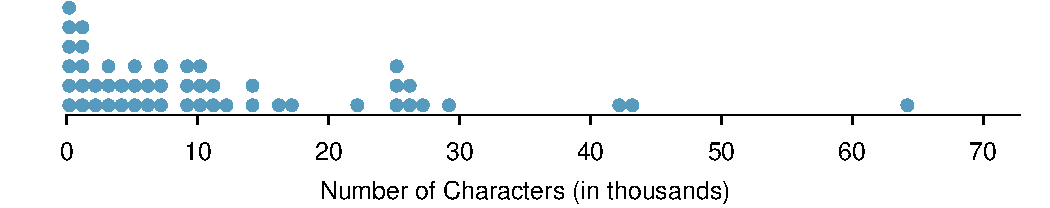
\includegraphics[width=0.825\textwidth]{ch_summarizing_data/figures/emailCharactersDotPlot/emailCharactersDotPlotStackedRounded}
   \caption{A dot plot of \var{num\_\hspace{0.3mm}char} for the \data{email50} data set.}
   \label{emailCharactersDotPlotStacked}
\end{figure}

\begin{exercisewrap}
\begin{nexercise}
Imagine rotating the dot plot 90 degrees clockwise. What do you notice?\footnotemark
\end{nexercise}
\end{exercisewrap}
\footnotetext{It has a similar shape as the stem-and-leaf plot! The values on the horizontal axis correspond to the stems and the number of dots in each interval correspond the number of leaves needed for each stem.}

These graphs make it easy to observe important features of the data, such as the location of clusters and presence of gaps.

\begin{examplewrap}
\begin{nexample}{Based on both the stem-and-leaf and dot plot, where are the values clustered and where are the gaps for the \data{email50} data set?}
There is a large cluster in the 0 to less than 20 thousand range, with a peak around 1 thousand. There are gaps between 30 and 40 thousand and between the two values in the 40 thousands and the largest value of approximately 64 thousand.
\end{nexample}
\end{examplewrap}

Additionally, we can easily identify any observations that appear to be unusually distant from the rest of the data. Unusually distant observations are called \termsub{outliers}{outlier}. Later in this chapter we will provide numerical rules of thumb for identifying outliers. For now, it is sufficient to identify them by observing gaps in the graph. In this case, it would be reasonable to classify the emails with character counts of 42 thousand, 43 thousand, and 64 thousand as outliers since they are numerically distant from most of the data.


\begin{onebox}{Outliers are extreme}
An \term{outlier} is an observation that appears extreme relative to the rest of the data.\end{onebox}


\begin{onebox}{Why it is important to look for outliers}
Examination of data for possible outliers serves many useful purposes, including\vspace{-2mm}
\begin{enumerate}
\setlength{\itemsep}{0mm}
\item Identifying asymmetry in the distribution.
\item Identifying data collection or entry errors. For instance, we re-examined the email purported to have 64 thousand characters to ensure this value was accurate.
\item Providing insight into interesting properties of the data.\vspace{0.5mm}
\end{enumerate}\end{onebox}

\begin{exercisewrap}
\begin{nexercise}
The observation 64 thousand, a suspected outlier, was found to be an accurate observation. What would such an observation suggest about the nature of character counts in emails?\footnotemark
\end{nexercise}
\end{exercisewrap}
\footnotetext{That occasionally there may be very long emails.}

\begin{exercisewrap}
\begin{nexercise}
Consider a data set that consists of the following numbers:  12, 12, 12, 12, 12, 13, 13, 14, 14, 15, 19. Which graph would better illustrate the data: a stem-and-leaf plot or a dot plot? Explain.\footnotemark
\end{nexercise}
\end{exercisewrap}
\footnotetext{Because all the values begin with 1, there would be only one stem (or two in a split stem-and-leaf). This would not provide a good sense of the distribution. For example, the gap between 15 and 19 would not be visually apparent. A dot plot would be better here.}

%%
\subsection{Histograms}
\label{histogramsAndShape}

Stem-and-leaf plots and dot plots are ideal for displaying data from small samples because they show the exact values of the observations and how frequently they occur. However, they are impractical for larger samples. For larger samples, rather than showing the frequency of every value, we prefer to think of the value as belonging to a \emph{bin}. For example, in the \data{email50} data set, we create a table of counts for the number of cases with character counts between 0 and 5,000, then the number of cases between 5,000 and 10,000, and so on. Such a table, shown in Figure~\ref{binnedNumCharTable}, is called a \term{frequency table}. Bins usually include the observations that fall on their left (lower) boundary and exclude observations that fall on their right (upper) boundary.  This is called \emph{left inclusive}. For example, 5 (i.e. 5000) would be counted in the 5-10 bin, not in the 0-5 bin.  These binned counts are plotted as bars in Figure~\ref{email50NumCharHist} into what is called a \term{histogram} or \term{frequency histogram}, which resembles the stacked dot plot shown in Figure~\ref{emailCharactersDotPlotStacked}.

\begin{figure}[ht]
\centering\small
\begin{tabular}{l ccc ccc ccc c}
  \hline
Characters & \\
(in thousands) & \raisebox{1.5ex}[0pt]{0-5} & \raisebox{1.5ex}[0pt]{5-10} & \raisebox{1.5ex}[0pt]{10-15} & \raisebox{1.5ex}[0pt]{15-20} & \raisebox{1.5ex}[0pt]{20-25} & \raisebox{1.5ex}[0pt]{25-30} & \raisebox{1.5ex}[0pt]{$\cdots$} & \raisebox{1.5ex}[0pt]{55-60} & \raisebox{1.5ex}[0pt]{60-65} \\
  \hline
Count & 19 & 12 & 6 & 2 & 3 & 5 & $\cdots$ & 0 & 1 \\
  \hline
\end{tabular}
\caption{The counts for the binned \var{num\_\hspace{0.3mm}char} data.}
\label{binnedNumCharTable}
\end{figure}

\begin{figure}[bth]
   \centering
    \oiRedirect{tableau-histogramschoose}{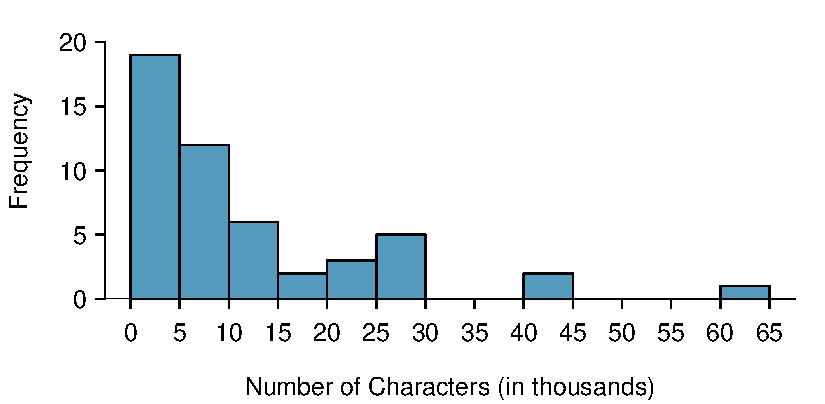
\includegraphics[width=0.82\textwidth]{ch_summarizing_data/figures/email50NumCharHist/email50NumCharHist}}
   \caption{A histogram of \var{num\_\hspace{0.3mm}char}. This histogram uses bins or class intervals of width 5.  Explore this histogram and dozens of histograms using American Community Survey data on Tableau Public~\tableauhref{tableau-histogramschoose}.}
   \label{email50NumCharHist}
\end{figure}

\begin{exercisewrap}
\begin{nexercise}
What can you see in the dot plot and stem-and-leaf plot that you cannot see in the frequency histogram?\footnotemark
\end{nexercise}
\end{exercisewrap}
\footnotetext{Character counts for individual emails.}

\begin{onebox}{Drawing histograms}
1. The variable is always placed on the horizontal axis. Before drawing the histogram, label both axes and draw a scale for each. \\[2mm]
2. Draw bars such that the height of the bar is the frequency of that bin and the width of the bar corresponds to the bin width.\end{onebox}

Histograms provide a view of the \term{data density}. Higher bars represent where the data are relatively more common. For instance, there are many more emails between 0 and 10,000 characters than emails between 10,000 and 20,000 in the data set. The bars make it easy to see how the density of the data changes relative to the number of characters.

\begin{examplewrap}
\begin{nexample}{How many emails had fewer than 10 thousand characters?}The height of the bars corresponds to frequency. There were 19 cases from 0 to less than 5 thousand and 12 cases from 5 thousand to less than 10 thousand, so there were $19+12=31$ emails with fewer than 10 thousand characters.
\end{nexample}
\end{examplewrap}

\begin{examplewrap}
\begin{nexample}{Approximately how many emails had fewer than 1 thousand chacters?} Based just on this histogram, we cannot know the exact answer to this question. We only know that 19 emails had between 0 and 5 thousand characters. If the number of emails is evenly distribution on this interval, then we can estimate that approximately 19/5~$\approx$ 4 emails fell in the range between 0 and 1 thousand.
\end{nexample}
\end{examplewrap}

\begin{examplewrap}
\begin{nexample}{What \emph{percent} of the emails had 10 thousand or more characters?}
From the first example, we know that 31 emails had fewer than 10 thousand characters. Since there are 50 emails in total, there must be 19 emails that have 10 thousand or more characters. To find the percent, compute $19/50 = 0.38 = 38\%$.
\end{nexample}
\end{examplewrap}

Sometimes questions such as the ones above can be answered more easily with a \term{cumulative frequency histogram}. This type of histogram shows cumulative, or total, frequency achieved by each bin, rather than the frequency in that particular bin.

\begin{figure}[ht]
\centering\small
\begin{tabular}{l ccc ccc ccc c}
  \hline
Characters & \\
(in thousands) & \raisebox{1.5ex}[0pt]{0-5} & \raisebox{1.5ex}[0pt]{5-10} & \raisebox{1.5ex}[0pt]{10-15} & \raisebox{1.5ex}[0pt]{15-20} & \raisebox{1.5ex}[0pt]{20-25} & \raisebox{1.5ex}[0pt]{25-30} &  \raisebox{1.5ex}[0pt]{30-35} &\raisebox{1.5ex}[0pt]{$\cdots$} & \raisebox{1.5ex}[0pt]{55-60} & \raisebox{1.5ex}[0pt]{60-65} \\
  \hline
Cumulative &\\
Frequency &  \raisebox{1.5ex}[0pt]{19} & \raisebox{1.5ex}[0pt]{31} & \raisebox{1.5ex}[0pt]{37} & \raisebox{1.5ex}[0pt]{39} & \raisebox{1.5ex}[0pt]{42} & \raisebox{1.5ex}[0pt]{47} & \raisebox{1.5ex}[0pt]{47} & \raisebox{1.5ex}[0pt]{$\cdots$} & \raisebox{1.5ex}[0pt]{49} & \raisebox{1.5ex}[0pt]{50} \\
  \hline
\end{tabular}
\caption{The cumulative frequencies for the binned \var{num\_\hspace{0.3mm}char} data.}
\label{binnedNumCharTableCumulative}
\end{figure}

\begin{figure}[h]
   \centering
\oiRedirect{tableau-histograms}{
   \Figures{0.82}{email50NumCharHist}{email50NumCharCumulativeFreqHist}}
   \caption{A cumulative frequency histogram of \var{num\_\hspace{0.3mm}char}. This histogram uses bins or class intervals of width 5.  Compare frequency, relative frequency, cumulative frequency, and cumulative relative frequency histograms on Tableau Public~\tableauhref{tableau-histograms}.}
   \label{email50NumCharCumulativeFreqHist}
\end{figure}

\begin{examplewrap}
\begin{nexample}{How many of the emails had fewer than 20 thousand characters?}
By tracing the height of the 15-20 thousand bin over to the vertical axis, we can see that it has a height just under 40 on the cumulative frequency scale. Therefore, we estimate that $\approx$39 of the emails had fewer than 30 thousand characters. Note that, unlike with a regular frequency histogram, we do not add up the height of the bars in a cumulative frequency histogram because each bar already represents a cumulative sum.
\end{nexample}
\end{examplewrap}

\begin{examplewrap}
\begin{nexample}{Using the cumulative frequency histogram, how many of the emails had 10-15 thousand characters?}
To answer this question, we do a subtraction. $\approx$39 had fewer than 15-20 thousand emails and $\approx$37 had fewer than 10-15 thousand emails, so $\approx$2 must have had between 10-15 thousand emails.
\end{nexample}
\end{examplewrap}

\begin{examplewrap}
\begin{nexample}{Approximately 25 of the emails had fewer than how many characters?}
This time we are given a cumulative frequency, so we start at 25 on the vertical axis and trace it across to see which bin it hits. It hits the 5-10 thousand bin, so 25 of the emails had fewer than a value somewhere between 5 and 10 thousand characters.
\end{nexample}
\end{examplewrap}

\D{\newpage}

Knowing that 25 of the emails had fewer than a value between 5 and 10 thousand characters is useful information, but it is even more useful if we know what percent of the total 25 represents. Knowing that there were 50 total emails tells us that $25 / 50 = 0.5 = 50\%$ of the emails had fewer than a value between 5 and 10 thousand characters. When we want to know what fraction or percent of the data meet a certain criteria, we use relative frequency instead of frequency. \termsub{Relative frequency}{relative frequency} is a fancy term for percent or proportion. It tells us how large a number is relative to the total.

Just as we constructed a frequency table, frequency histogram, and cumulative frequency histogram, we can construct a relative frequency table, relative frequency histogram, and cumulative relative frequency histogram.

\begin{exercisewrap}
\begin{nexercise}
How will the \emph{shape} of the relative frequency histograms differ from the frequency histograms?\footnotemark
\end{nexercise}
\end{exercisewrap}
\footnotetext{The shape will remain exactly the same. Changing from frequency to relative frequency involves dividing all the frequencies by the same number, so only the vertical scale (the numbers on the y-axis) change.}

\begin{onebox}{Pay close attention to the vertical axis of a histogram}
{We can misinterpret a histogram if we forget to check whether the vertical axis represents frequency, relative frequency, cumulative frequency, or cumulative relative frequency.}
\end{onebox}

%\Comment{insert relative frequency table and relative frequency histogram here?}

%\Comment{reference the relative frequency graph here since it is closer}


%%
\subsection{Describing Shape}
\label{shape}

Frequency and relative frequency histograms are especially convenient for describing the \term{shape} of the data distribution\label{shapeFirstDiscussed}. Figure~\ref{email50NumCharHist} shows that most emails have a relatively small number of characters, while fewer emails have a very large number of characters. When data trail off to the right in this way and have a longer right \hiddenterm{tail}\index{skew!tail}, the shape is said to be \termsub{right skewed}{skew!right skewed}.\footnote{Other ways to describe data that are right skewed: \termni{skewed to the right}, \termni{skewed to the high end}, or \termni{skewed to the positive end}.}

Data sets with the reverse characteristic -- a long, thin tail to the left -- are said to be \termsub{left skewed}{skew!left skewed}. We also say that such a distribution has a long left tail. Data sets that show roughly equal trailing off in both directions are called \term{symmetric}.\index{skew!symmetric}

\begin{onebox}{Long tails to identify skew}
When data trail off in one direction, the distribution has a \term{long tail}. \index{skew!long tail|textbf} If a distribution has a long left tail, it is left skewed. If a distribution has a long right tail, it is right skewed.\end{onebox}

\begin{exercisewrap}
\begin{nexercise}
Take a look at the dot plot in Figure~\ref{emailCharactersDotPlotStacked}. Can you see the skew in the data? Is it easier to see the skew in the frequency histogram, the dot plot, or the stem-and-leaf plot?\footnotemark
\end{nexercise}
\end{exercisewrap}
\footnotetext{The skew is visible in all three plots. However, it is not easily visible in the cumulative frequency histogram.}

\begin{exercisewrap}
\begin{nexercise}
Would you expect the distribution of number of pets per household to be right skewed, left skewed, or approximately symmetric?  Explain.\footnotemark
\end{nexercise}
\end{exercisewrap}
\footnotetext{We suspect most households would have 0, 1, or 2 pets but that a smaller number of households will have 3, 4, 5, or more pets, so there will be greater density over the small numbers, suggesting the distribution will have a long right tail and be right skewed.}

\D{\newpage}

In addition to looking at whether a distribution is skewed or symmetric, histograms, stem-and-leaf plots, and dot plots can be used to identify modes. A \term{mode} is represented by a prominent peak in the distribution.\footnote{Another definition of mode, which is not typically used in statistics, is the value with the most occurrences. It is common to have \emph{no} observations with the same value in a data set, which makes this other definition useless for many real data sets.} There is only one prominent peak in the histogram of \var{num\_\hspace{0.3mm}char}.

Figure~\ref{singleBiMultiModalPlots} shows histograms that have one, two, or three prominent peaks. Such distributions are called \termsub{unimodal}{modality!unimodal}, \termsub{bimodal}{modality!bimodal}, and \termsub{multimodal}{modality!multimodal}, respectively. Any distribution with more than 2 prominent peaks is called multimodal. Notice that in Figure~\ref{email50NumCharHist} there was one prominent peak in the unimodal distribution with a second less prominent peak that was not counted since it only differs from its neighboring bins by a few observations.

\begin{figure}[h]
   \centering
   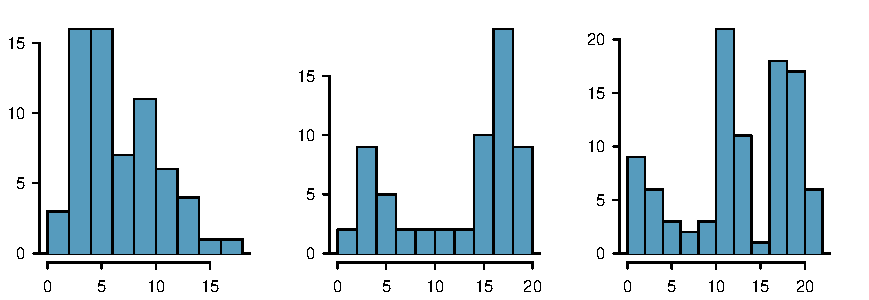
\includegraphics[width=\textwidth]{ch_summarizing_data/figures/singleBiMultiModalPlots/singleBiMultiModalPlots}
   \caption{Counting only prominent peaks, the distributions are (left to right) unimodal, bimodal, and multimodal.}
   \label{singleBiMultiModalPlots}
\end{figure}

\begin{exercisewrap}
\begin{nexercise}
Height measurements of young students and adult teachers at a K-3 elementary school were taken. How many modes would you anticipate in this height data set?\footnotemark
\end{nexercise}
\end{exercisewrap}
\footnotetext{There might be two height groups visible in the data set: one of the students and one of the adults. That is, the data are probably bimodal.}

\begin{onebox}{Looking for modes}
Looking for modes isn't about finding a clear and correct answer about the number of modes in a distribution, which is why \emph{prominent} is not rigorously defined in this book. The important part of this examination is to better understand your data and how it might be structured.\end{onebox}

\subsection{Descriptive versus inferential statistics}

Finally, we note that the graphical summaries of this section and the numerical summaries of the next section fall into the realm of \term{descriptive statistics}.  Descriptive statistics is about describing or summarizing data; it does not attribute properties of the data to a larger population.  \termsub{Inferential statistics}{inferential statistics}, on the other hand, uses samples to generalize or to infer something about a larger population.  We will have to wait until Chapter~5 to enter the exciting world of inferential statistics.

\D{\newpage}

%%
\subsection*{Section summary}

\begin{itemize}
  \item A \term{scatterplot} is a \term{bivariate} display illustrating the relationship between two numerical variables.  The observations must be \term{paired}, which is to say that they correspond to the same case or individual.  The linear association between two variables can be positive or negative, or there can be no association. \termsub{Positive association}{positive association} means that larger values of the first variable are associated with larger values of the second variable. \termsub{Negative association}{negative association} means that larger values of the first variable are associated with smaller values of the second variable.  Additionally, the association can follow a linear trend or a curved (nonlinear) trend.
  \item When looking at a \term{univariate} display, researchers want to understand the distribution of the variable.  The term \term{distribution} refers to the values that a variable takes and the frequency of those values.  When looking at a distribution, note the presence of clusters, gaps, and \termsub{outliers}{outlier}.
\item Distributions may be \term{symmetric} or they may have a long tail.  If a distribution has a long left tail (with greater density over the higher numbers), it is \term{left skewed}. If a distribution has a long right tail (with greater density over the smaller numbers), it is \term{right skewed}.
\item Distributions may be \term{unimodal}, \term{bimodal}, or \term{multimodal}.  
\item Two graphs that are useful for showing the distribution of a small number of observations are the \term{stem-and-leaf plot} and \term{dot plot}.  These graphs are ideal for displaying data from small samples because they show the exact values of the observations and how frequently they occur. However, they are impractical for larger data sets. 
\item For larger data sets it is common to use a \term{frequency histogram} or a \term{relative frequency histogram} to display the distribution of a variable.  This requires choosing bins of an appropriate width.
\item To see cumulative amounts, use a \term{cumulative frequency histogram}.  A \term{cumulative relative frequency histogram} is ideal for showing \termsub{percentiles}{percentile}.
\item \termsub{Descriptive statistics}{descriptive statistics} describes or summarizes data, while \term{inferential statistics} uses samples to generalize or infer something about a larger population.
\end{itemize}



%\Comment{maybe a separate section here on numerical summaries of (numerical) data}


%%%%%%%%%%%Section Exercises
{\exercisesheader{}


% 1

\eoce{\qt{ACS, Part I} Each year, the US Census Bureau surveys about 3.5 million households with The American Community Survey (ACS). Data collected from the ACS have been crucial in government and policy decisions, helping to determine the allocation of federal and state funds each year. Some of the questions asked on the survey are about their income, age (in years), and gender. The table below contains this information for a random sample of 20 respondents to the 2012 ACS. \footfullcite{data:acs:2012} \label{acs_age_income}
\begin{center}
\begin{minipage}[c]{0.4\textwidth}
{\small
\begin{tabular}{rrrl}
  \hline
 & Income & Age & Gender \\ 
  \hline
1 & 53,000 &  28 & male \\ 
  2 & 1600 &  18 & female \\ 
  3 & 70,000 &  54 & male \\ 
  4 & 12,800 &  22 & male \\ 
  5 & 1,200 &  18 & female \\ 
  6 & 30,000 &  34 & male \\ 
  7 & 4,500 &  21 & male \\ 
  8 & 20,000 &  28 & female \\ 
  9 & 25,000 &  29 & female \\ 
  10 & 42,000 &  33 & male \\ 
   \hline
\end{tabular}
}
\end{minipage}
\begin{minipage}[c]{0.4\textwidth}
{\small
\begin{tabular}{rrrl}
  \hline
 & Income & Age & Gender \\ 
  \hline
  11 & 670 &  34 & female \\ 
  12 & 29,000 &  55 & female \\ 
  13 & 44,000 &  33 & female \\ 
  14 & 48,000 &  41 & male \\ 
  15 & 30,000 &  47 & female \\ 
  16 & 60,000 &  30 & male \\ 
  17 & 108,000 &  61 & male \\ 
  18 & 5,800 &  50 & female \\ 
  19 & 50,000 &  24 & female \\ 
  20 & 11,000 &  19 & male \\ 
   \hline
\end{tabular}
}
\end{minipage}
\end{center}
\begin{parts}
\item Create a scatterplot of income vs. age, and describe the relationship between these two variables.
\item Now create two scatterplots: one for income vs. age for males and another for females.
\item How, if at all, do the relationships between income and age differ for males and females?
\end{parts}
}{}

% 2

\eoce{\qt{MLB stats} A baseball team's success in a season is usually measured by their number of wins. In order to win, the team has to have scored more points (runs) than their opponent in any given game. As such, number of runs is often a good proxy for the success of the team. The table below shows number of runs, home runs, and batting averages for a random sample of 10 teams in the 2014 Major League Baseball season. \footfullcite{data:MLB:2014}
\begin{center}
{\small
\begin{tabular}{rlrrr}
  \hline
 & Team & Runs & Home runs & Batting avg. \\ 
  \hline
1 & Baltimore &  705 &  211 & 0.256 \\ 
  2 & Boston &  634 &  123 & 0.244 \\ 
  3 & Cincinnati &  595 &  131 & 0.238 \\ 
  4 & Cleveland &  669 &  142 & 0.253 \\ 
  5 & Detroit &  757 &  155 & 0.277 \\ 
  6 & Houston &  629 &  163 & 0.242 \\ 
  7 & Minnesota &  715 &  128 & 0.254 \\ 
  8 & NY Yankees &  633 &  147 & 0.245 \\ 
  9 & Pittsburgh &  682 &  156 & 0.259 \\ 
  10 & San Francisco &  665 &  132 & 0.255 \\ 
   \hline
\end{tabular}
}
\end{center}
\begin{parts}
\item Draw a scatterplot of runs vs. home runs.
\item Draw a scatterplot of runs vs. batting averages.
\item Are home runs or batting averages more strongly associated with number of runs? Explain your reasoning.
\end{parts}
}{}

% 3

\eoce{\qt{Fiber in your cereal} \label{fiber_cereal} The Cereal FACTS report provides information on nutrition content of cereals as well as who they are targeted for (adults, children, families). We have selected a random sample of 20 cereals from the data provided in this report. Shown below are the fiber contents (percentage of fiber per gram of cereal) for these cereals. \footfullcite{Harris:2012}
\begin{center}
\begin{minipage}[c]{0.49\textwidth}
{\small
\begin{tabular}{rlr}
  \hline
 & Brand & Fiber \% \\ 
  \hline
1 & Pebbles Fruity & 0.0\% \\ 
  2 & Rice Krispies Treats & 0.0\% \\ 
  3 & Pebbles Cocoa & 0.0\% \\ 
  4 & Pebbles Marshmallow & 0.0\% \\ 
  5 & Frosted Rice Krispies & 0.0\% \\ 
  6 & Rice Krispies  & 3.0\% \\ 
  7 & Trix  & 3.1\% \\ 
  8 & Honey Comb  & 3.1\% \\ 
  9 & Rice Krispies Gluten Free & 3.3\% \\ 
  10 & Frosted Flakes  & 3.3\% \\ 
   \hline
\end{tabular}
}
\end{minipage}  
 \begin{minipage}[c]{0.49\textwidth}
{\small
\begin{tabular}{rlr}
  \hline
 & Brand & Fiber \% \\ 
   \hline 
  11 & Cinnamon Toast Crunch & 3.3\% \\ 
  12 & Reese's Puffs  & 3.4\% \\ 
  13 & Cheerios Honey Nut & 7.1\% \\ 
  14 & Lucky Charms  & 7.4\% \\ 
  15 & Pebbles Boulders Chocolate PB & 7.4\% \\ 
  16 & Corn Pops  & 9.4\% \\ 
  17 & Frosted Flakes Reduced Sugar & 10.0\% \\ 
  18 & Clifford Crunch  & 10.0\% \\ 
  19 & Apple Jacks  & 10.7\% \\ 
  20 & Dora the Explorer  & 11.1\% \\ 
   \hline
\end{tabular}
}
\end{minipage}  
\end{center}
\begin{parts}
\item Create a stem and leaf plot of the distribution of the fiber content of these cereals.
\item Create a dot plot of the fiber content of these cereals.
\item Create a histogram and a relative frequency histogram of the fiber content of these cereals.
\item What percent of cereals contain more than 7\% fiber?
\end{parts}
}{}

% 4

\eoce{\qt{Sugar in your cereal} The Cereal FACTS report from Exercise~\ref{fiber_cereal} also provides information on sugar content of cereals. We have selected a random sample of 20 cereals from the data provided in this report. Shown below are the sugar contents (percentage of sugar per gram of cereal) for these cereals.
\begin{center}
\begin{minipage}[c]{0.49\textwidth}
{\small
\begin{tabular}{rlr}
  \hline
 & Brand & Sugar \% \\ 
  \hline
1 & Rice Krispies Gluten Free & 3\% \\ 
  2 & Rice Krispies  & 12\% \\ 
  3 & Dora the Explorer  & 22\% \\ 
  4 & Frosted Flakes Red. Sugar & 27\% \\ 
  5 & Clifford Crunch  & 27\% \\ 
  6 & Rice Krispies Treats & 30\% \\ 
  7 & Pebbles Boulders Choc. PB & 30\% \\ 
  8 & Cinnamon Toast Crunch & 30\% \\ 
  9 & Trix  & 31\% \\ 
  10 & Honey Comb  & 31\% \\ 
   \hline
\end{tabular}
}
\end{minipage}  
 \begin{minipage}[c]{0.49\textwidth}
{\small
\begin{tabular}{rlr}
  \hline
 & Brand & Sugar \% \\ 
   \hline 
  11 & Corn Pops  & 31\% \\ 
  12 & Cheerios Honey Nut & 32\% \\ 
  13 & Reese's Puffs  & 34\% \\ 
  14 & Pebbles Fruity & 37\% \\ 
  15 & Pebbles Cocoa & 37\% \\ 
  16 & Lucky Charms  & 37\% \\ 
  17 & Frosted Flakes  & 37\% \\ 
  18 & Pebbles Marshmallow & 37\% \\ 
  19 & Frosted Rice Krispies & 40\% \\ 
  20 & Apple Jacks  & 43\% \\
   \hline
\end{tabular}
}
\end{minipage}  
\end{center}
\begin{parts}
\item Create a stem and leaf plot of the distribution of the sugar content of these cereals.
\item Create a dot plot of the sugar content of these cereals.
\item Create a histogram and a relative frequency histogram of the sugar content of these cereals.
\item What percent of cereals contain more than 30\% sugar?
\end{parts}
}{}


% 5

\eoce{\qt{Mammal life spans\label{mammal_life_spans}} Data were collected on life spans (in 
years) and gestation lengths (in days) for 62 mammals. A scatterplot of life span versus 
length of gestation is shown below. \footfullcite{Allison+Cicchetti:1975}

\noindent\begin{minipage}[c]{0.44\textwidth}
\begin{parts}
\item What type of an association is apparent between life span and length of gestation?
\item What type of an association would you expect to see if the axes of the plot were reversed, i.e. if we plotted length of gestation versus life span?
\item Are life span and length of gestation independent? Explain your reasoning.
\end{parts}
\end{minipage}
\begin{minipage}[c]{0.55\textwidth}
\begin{center}
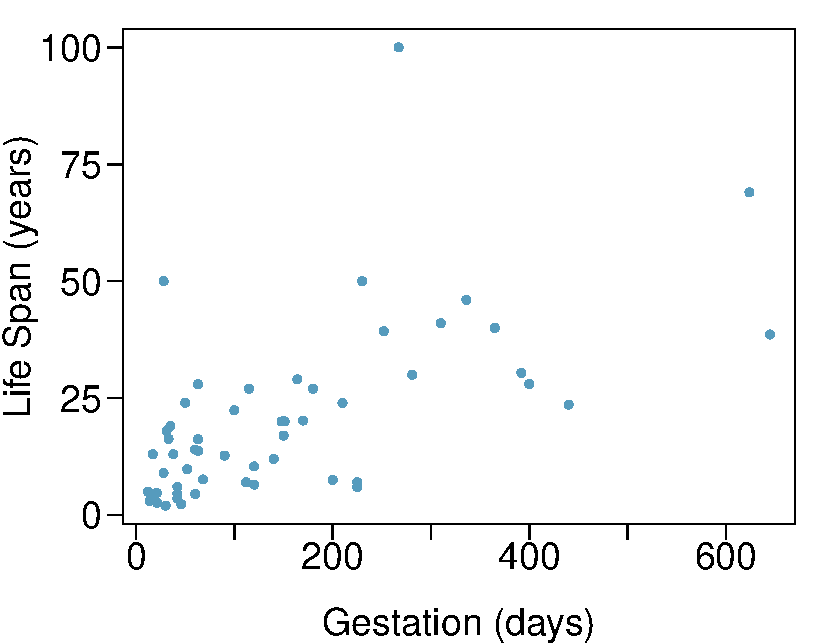
\includegraphics[width = 0.86\textwidth]{ch_summarizing_data/figures/eoce/mammal_life_spans/mammal_life_spans_scatterplot.pdf}
\end{center}
\end{minipage}
}{}

% 6

\eoce{\qt{Associations\label{association_plots}}
Indicate which of the plots show
(a)~a positive association,
(b)~a negative association, or
(c)~no~association.
Also determine if the positive and negative associations
are linear or nonlinear.
Each part may refer to more than one plot.
\begin{center}
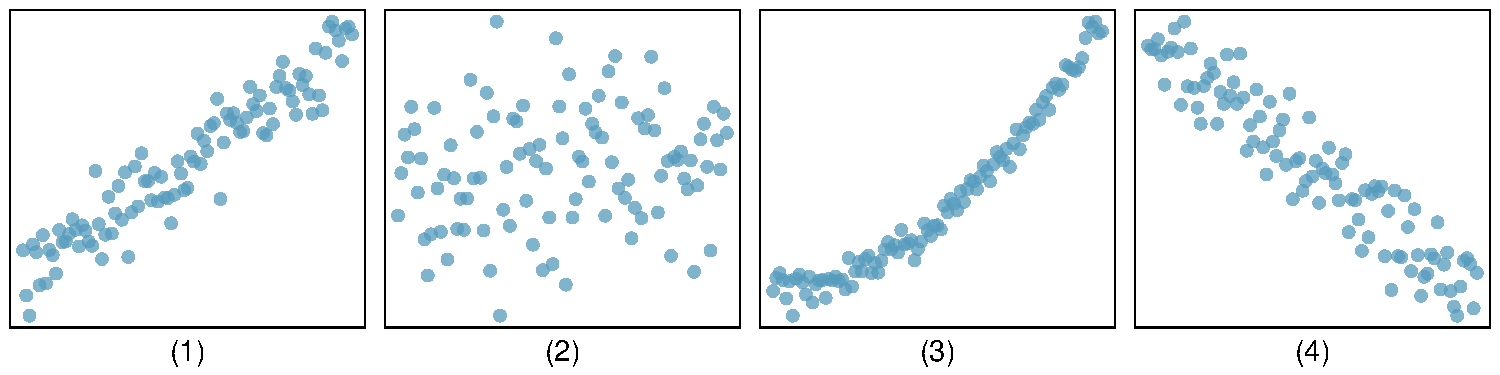
\includegraphics[width = 0.95\textwidth]{ch_summarizing_data/figures/eoce/association_plots/association_plots.pdf}
\end{center}
}{}

}

%______________________________________________
\section[Numerical summaries and box plots]{Numerical summaries and box plots }
\label{numericalSummariesAndBoxPlots}

\sectionintro{
\noindent%
What are the different ways to measure the center of
a distribution, and why is there more than one way to
measure the center?
How do you know if a value is ``far" from the center?  What does it mean to an outlier?  We will continue with the \data{email50} data set and investigate multiple quantitative summarizes for numerical data.

%%
\subsection{Learning objectives}
\begin{enumerate}
\setlength{\itemsep}{0mm}
\item Calculate, interpret, and compare the two measures of center (mean and median) and the three  measures of spread (standard deviation, interquartile range, and range).

\item Understand how the shape of a distribution affects the relationship between the mean and the median.

\item Identify and apply the two rules of thumb for identify outliers (one involving standard deviation and mean and the other involving $Q_1$ and $Q_3$).

\item Describe the distribution a numerical variable with respect to center, spread, and shape, noting the presence of outliers.
  
\item Find the 5 number summary and IQR, and draw a box plot with outliers shown.

\item Understand the effect changing units has on each of the summary quantities.

\item Use the empirical rule to summarize approximately normal distributions.

\item Use quartiles, percentiles, and Z-scores to measure the relative position of a data point within the data set.

\item Compare the distribution of a numerical variable using dot plots / histograms with the same scale, back-to-back stem-and-leaf plots, or parallel box plots.  Compare the distributions with respect to center, spread, shape, and outliers.

\end{enumerate}
}


%%
\subsection{Measures of center}
\label{center}

In the previous section, we saw that modes can occur anywhere in a data set. Therefore, mode is not a measure of \term{center}. We understand the term \emph{center} intuitively, but quantifying what is the center can be a little more challenging. This is because there are different definitions of center. Here we will focus on the two most common: the mean and median.

The \term{mean}, sometimes called the \indexthis{average}{mean!average}, is a common way to measure the center of a distribution of data. To find the mean number of characters in the 50 emails, we add up all the character counts and divide by the number of emails. For computational convenience, the number of characters is listed in the thousands and rounded to the first decimal.
\begin{eqnarray*}
\bar{x} = \frac{21.7 + 7.0 + \cdots + 15.8}{50} = 11.6
\label{sampleMeanEquation}
\end{eqnarray*}
The sample mean is often labeled $\bar{x}$. The letter $x$ is being used as a generic placeholder for the variable of interest, \var{num\_\hspace{0.3mm}char}, and the bar on the $x$ communicates that the average number of characters in the 50 emails was 11,600.

\begin{onebox}{Mean}
The sample mean of a numerical variable is computed as the sum of all of the observations divided by the number of observations:
\begin{eqnarray*}
\bar{x} = \frac{1}{n}\sum{x_{i}} = \frac{\sum{x_i}}{n}=\frac{x_1+x_2+\cdots+x_n}{n}
\label{meanEquation}
\end{eqnarray*}
where $\sum$ is the capital Greek letter sigma and $\sum{x_{i}}$ means take the sum of all the individual $x$ values.
 $x_1, x_2, \dots, x_n$ represent the $n$ observed values.\end{onebox}

\begin{exercisewrap}
\begin{nexercise}
Examine Equations~\eqref{sampleMeanEquation} and~\eqref{meanEquation} above. What does $x_1$ correspond to? And $x_2$? What does $x_i$ represent?\footnotemark
\end{nexercise}
\end{exercisewrap}
\footnotetext{$x_1$ corresponds to the number of characters in the first email in the sample (21.7, in thousands), $x_2$ to the number of characters in the second email (7.0, in thousands), and $x_i$ corresponds to the number of characters in the $i^{th}$ email in the data set.}

\begin{exercisewrap}
\begin{nexercise}
What was $n$ in this sample of emails?\footnotemark
\end{nexercise}
\end{exercisewrap}
\footnotetext{The sample size was $n=50$.}

The \data{email50} data set represents a sample from a larger population of emails that were received in January and March. We could compute a mean for this population in the same way as the sample mean, however, the population mean has a special label: $\mu$. \index{Greek!mu@mu ($\mu$)} The symbol $\mu$ is the Greek letter \emph{mu} and represents the average of all observations in the population. Sometimes a subscript, such as $_x$, is used to represent which variable the population mean refers to, e.g. $\mu_x$.

\begin{examplewrap}
\begin{nexample}{The average number of characters across all emails can be estimated using the sample data. Based on the sample of 50 emails, what would be a reasonable estimate of $\mu_x$, the mean number of characters in all emails in the \data{email} data set? (Recall that \data{email50} is a sample from \data{email}.)}
The sample mean, 11,600, may provide a reasonable estimate of $\mu_x$. While this number will not be perfect, it provides a \emph{point estimate} of the population mean. In Chapter~\ref{foundationsForInference} and beyond, we will develop tools to characterize the reliability of point estimates, and we will find that point estimates based on larger samples tend to be more reliable than those based on smaller samples.
\end{nexample}
\end{examplewrap}

\begin{examplewrap}
\begin{nexample}{We might like to compute the average income per person in the US. To do so, we might first think to take the mean of the per capita incomes across the 3,142 counties in the \data{county} data set. What would be a better approach?} \label{wtdMeanOfIncome}
The \data{county} data set is special in that each county actually represents many individual people. If we were to simply average across the \var{income} variable, we would be treating counties with 5,000 and 5,000,000 residents equally in the calculations. Instead, we should compute the total income for each county, add up all the counties' totals, and then divide by the number of people in all the counties. If we completed these steps with the \data{county} data, we would find that the per capita income for the US is \$27,348.43. Had we computed the \emph{simple} mean of per capita income across counties, the result would have been just \$22,504.70!
\end{nexample}
\end{examplewrap}

Example~\ref{wtdMeanOfIncome} used what is called a \term{weighted mean}\index{mean!weighted mean}, which will not be a key topic in this textbook. However, we have provided an online supplement on weighted means for interested readers:
\begin{center}
\oiRedirect{textbook-weighted_mean_supplement}{www.openintro.org/stat/down/supp/wtdmean.pdf}
\end{center}

The median provides another measure of center. The \term{median} splits an ordered data set in half. There are 50 character counts in the \data{email50} data set (an even number) so the data are perfectly split into two groups of~25. We take the median in this case to be the average of the two middle observations: $(\text{6,768} + \text{7,012}) / 2 = \text{6,890}$. When there are an odd number of observations, there will be exactly one observation that splits the data into two halves, and in this case that observation is the median (no average needed).

\begin{onebox}{Median: the number in the middle}
In an ordered data set, the \term{median} is the observation right in the middle. If there are an even number of observations, the median is the average of the two middle values.\end{onebox}

Graphically, we can think of the mean as the balancing point. The median is the value such that 50\% of the \emph{area} is to the left of it and 50\% of the \emph{area} is to the right of it.

%\Comment{insert histogram of email data set with mean and median indicated}.

\begin{figure}[h]
   \centering
   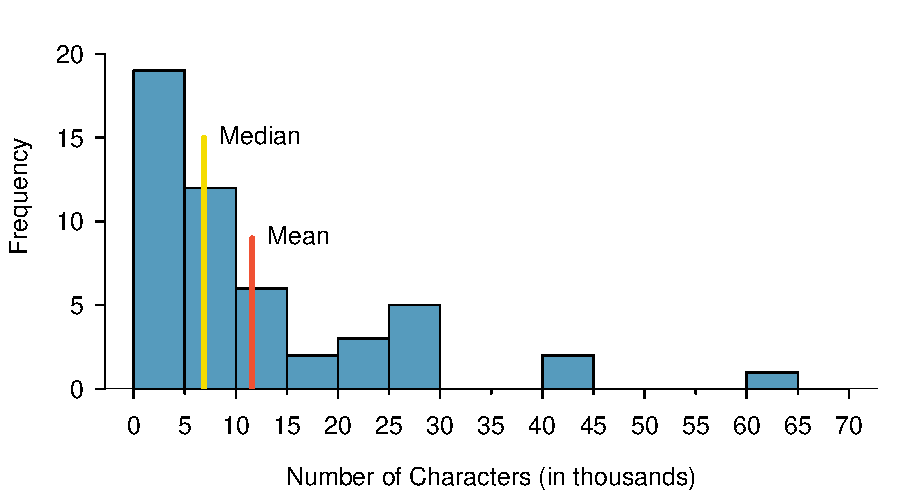
\includegraphics[width=0.8\textwidth]{ch_summarizing_data/figures/email50NumCharHist/email50NumCharHistWMeanMedian}
   \caption{A histogram of \var{num\_\hspace{0.3mm}char} with its mean and median shown.}
   \label{email50NumCharHistWMeanMedian}
\end{figure}

\begin{examplewrap}
\begin{nexample}{Based on the data, why is the mean greater than the median in this data set?}
Consider the three largest values of 42 thousand, 43 thousand, and 64 thousand. These values drag up the mean because they substantially increase the sum (the~total). However, they do not drag up the median because their magnitude does not change the location of the middle value.
\end{nexample}
\end{examplewrap}

%\Comment{add box}.

\begin{onebox}{The mean follows the tail}
In a right skewed distribution, the mean is greater than the median.

In a left skewed distribution, the mean is less than the median.

In a symmetric distribution, the mean and median are approximately equal.\end{onebox}

\begin{exercisewrap}
\begin{nexercise}Consider the distribution of individual income in the United States. Which is greater: the mean or median? Why?\footnotemark
\end{nexercise}
\end{exercisewrap}
\footnotetext{Because a small percent of individuals earn extremely large amounts of money while the majority earn a modest amount, the distribution is skewed to the right. Therefore, the mean is greater than the median.}


\D{\newpage}

%%
\subsection{Standard deviation as a measure of spread}
\label{variability}

The U.S. Census Bureau reported that in 2017, the median family income was \$73,891 and the mean family income was \$99,114.\footnote{\oiRedirect{factfinder-gov-income2}{\mbox{\url{https://factfinder.census.gov/faces/tableservices/jsf/pages/productview.xhtml?pid=ACS_17_1YR_S1901}}}} Is a family income of \$60,000 far from the mean or somewhat close to the mean? In order to answer this question, it is not enough to know the center of the data set and its \term{range} (maximum value - minimum value). We must know about the variability\index{variability} of the data set within that range. Low variability or small spread means that the values tend to be more clustered together. High variability or large spread means that the values tend to be far apart.

\begin{examplewrap}
\begin{nexample}{Is it possible for two data sets to have the same range but different spread? If so, give an example. If not, explain why not.}
Yes. An example is:  {1, 1, 1, 1, 1, 9, 9, 9, 9, 9} and {1, 5, 5, 5, 5, 5, 5, 5, 5, 5, 9}.

The first data set has a larger spread because values tend to be farther away from each other while in the second data set values are clustered together at the mean.
\end{nexample}
\end{examplewrap}

Here, we introduce the standard deviation as a measure of spread. Though its formula is a bit tedious to calculate by hand, the standard deviation is very useful in data analysis and roughly describes how far away, on average, the observations are from the mean.

We call the distance of an observation from its mean its \term{deviation}. Below are the deviations for the $1^{st}_{}$, $2^{nd}_{}$, $3^{rd}$, and $50^{th}_{}$ observations in the \var{num\_\hspace{0.3mm}char} variable. For computational convenience, the number of characters is listed in the thousands and rounded to the first decimal.
\begin{align*}
x_1^{}-\bar{x} &= 21.7 - 11.6 = 10.1 \hspace{5mm}\text{ } \\
x_2^{}-\bar{x} &= 7.0 - 11.6 = -4.6 \\
x_3^{}-\bar{x} &= 0.6 - 11.6 = -11.0 \\
			&\ \vdots \\
x_{50}^{}-\bar{x} &= 15.8 - 11.6 = 4.2
\end{align*}
% library(openintro); d <- email50$num_char; round(mean(d),1); d[c(1,2,3,50)]; d[c(1,2,3,50)] - round(mean(d),1); (d[c(1,2,3,50)] - round(mean(d)))^2; sum((d - round(mean(d)))^2)/49; sqrt(sum((d - round(mean(d)))^2)/49); var(d); sd(d)
If we square these deviations and then take an average, the result is about equal to the sample \term{variance}\label{varianceIsDefined}, denoted by $s_{}^2$:
\begin{align*}
s_{}^2 &= \frac{10.1_{}^2 + (-4.6)_{}^2 + (-11.0)_{}^2 + \cdots + 4.2_{}^2}{50-1} \\
	&= \frac{102.01 + 21.16 + 121.00 + \cdots + 17.64}{49} \\
	&= 172.44
\end{align*}
We divide by $n-1$, rather than dividing by $n$, when computing the variance; you need not worry about this mathematical nuance for the material in this textbook. Notice that squaring the deviations does two things. First, it makes large values much larger, seen by comparing $10.1^2$, $(-4.6)^2$, $(-11.0)^2$, and $4.2^2$. Second, it gets rid of any negative signs.

The \term{standard deviation} is defined as the square root of the variance:
$$s=\sqrt{172.44} = 13.13$$

The standard deviation of the number of characters in an email is about 13.13 thousand. A subscript of $_x$ may be added to the variance and standard deviation, i.e. $s_x^2$ and $s_x^{}$, as a reminder that these are the variance and standard deviation of the observations represented by $x_1^{}$, $x_2^{}$, ..., $x_n^{}$. The $_{x}$ subscript is usually omitted when it is clear which data the variance or standard deviation is referencing.

%\Add{The variance is roughly the average squared distance from the mean and the standard deviation is the square root of the variance.}

\D{\newpage}

\begin{onebox}{Calculating the standard deviation}
The standard deviation is the square root of the variance. It is roughly the ``typical" distance of the observations from the mean.
\begin{eqnarray*}
\label{sdEquation}
s_{\scriptscriptstyle{X}}
 = \sqrt{\frac{1}{n-1} \sum{(x_i -  \bar{x})^2}}
\end{eqnarray*}
\end{onebox}

The variance is useful for mathematical reasons, but the standard deviation is easier to interpret because it has the same units as the data set. The units for variance will be the units squared (e.g. meters$^2$).
Formulas and methods used to compute the variance and standard deviation for a population are similar to those used for a sample.\footnote{The only difference is that the population variance has a division by $n$ instead of $n-1$.} However, like the mean, the population values have special symbols: $\sigma_{}^2$ for the variance and $\sigma$ for the standard deviation. The symbol $\sigma$ \index{Greek!sigma@sigma ($\sigma$)} is the Greek letter \emph{sigma}.

\begin{onebox}{thinking about the standard deviation}
It is useful to think of the standard deviation as the ``typical" or ``average" distance that observations fall from the mean.\end{onebox}

In Chapter~4, we encounter a bell-shaped distribution known as the \emph{normal distribution}.  The \term{empirical rule} tells us that for normal distributions, about 68\% of the data will be within one standard deviation of the mean, about 95\% will be within two standard deviations of the mean, and about 99.7\% will be within three standard deviations of the mean. However, as seen in Figures~\ref{emailCharactersDotPlotStackedRoundedWithSD} and~\ref{severalDiffDistWithSdOf1}, these percentages generally do not hold if the distribution is not bell-shaped.  

\begin{figure}[h]
\centering
\Figures{}{emailCharactersDotPlot}
    {emailCharactersDotPlotStackedRoundedWithSD}
\caption{In the \var{num\_\hspace{0.3mm}char} data, 40 of the 50 emails (80\%) are within 1~standard deviation of the mean, and 47 of the 50 emails (94\%) are within 2 standard deviations. The empirical rule does not hold well for skewed data, as shown in this example.}
\label{emailCharactersDotPlotStackedRoundedWithSD}
\end{figure}

\begin{figure}
\centering
\Figure{0.7}{severalDiffDistWithSdOf1}
\caption{Three very different population distributions with the same mean $\mu=0$ and standard deviation $\sigma=1$.}
\label{severalDiffDistWithSdOf1}
\end{figure}

\begin{exercisewrap}
\begin{nexercise}
On page~\pageref{shapeFirstDiscussed}, the concept of shape of a distribution was introduced. A good description of the shape of a distribution should include modality and whether the distribution is symmetric or skewed to one side. Using Figure~\ref{severalDiffDistWithSdOf1} as an example, explain why such a description is important.\footnotemark
\end{nexercise}
\end{exercisewrap}
\footnotetext{Figure~\ref{severalDiffDistWithSdOf1} shows three distributions that look quite different, but all have the same mean, variance, and standard deviation. Using modality, we can distinguish between the first plot (bimodal) and the last two (unimodal). Using skewness, we can distinguish between the last plot (right skewed) and the first two. While a picture, like a histogram, tells a more complete story, we can use modality and shape (symmetry/skew) to characterize basic information about a~distribution.}

\D{\newpage}

\begin{examplewrap}
\begin{nexample}{Earlier we reported that the mean family income in the U.S. in 2017 was \$99,114. Estimating the standard deviation of income as approximately \$50,000, is a family income of \$60,000 far from the mean or relatively close to the mean?}
Because \$60,000 is less that one standard deviation from the mean, it is relatively close to the mean. If the value were more than 2 standard deviations away from the mean, we would consider it far from the mean.
\end{nexample}
\end{examplewrap}

When describing any distribution, comment on the three important characteristics of center, spread, and shape. Also note any especially unusual cases.


\begin{examplewrap}
\begin{nexample}{In the data's context (the number of characters in emails), describe the distribution of the \var{num\_\hspace{0.3mm}char} variable shown in the histogram below.
  \begin{center}
   \Figure{0.65}{email50NumCharHist}
  \end{center}}
The distribution of email character counts is unimodal and very strongly skewed to the right. Many of the counts fall near the mean at 11,600, and most fall within one standard deviation (13,130) of the mean. There is one exceptionally long email with about 65,000 characters.



\end{nexample}
\end{examplewrap}

In this chapter we use standard deviation as a descriptive statistic to describe the variability in a given data set. In Chapter~\ref{foundationsForInference} we will use the standard deviation to assess how close a sample mean is to the population mean.


\D{\newpage}

%%
\subsection{Z-scores}



Knowing how many standard deviations a value is from the mean is often more useful than simply knowing how far a value is from the mean.

\begin{examplewrap}
\begin{nexample}
{Consider that the mean family income in the U.S. in 2017 was \$99,114. Let's round this to \$100,000 and estimate the standard deviation of income as \$50,000.  Using these estimates, how many standard deviations above the mean is an income of \$200,000?  }
The value \$200,000 is \$100,000 above the mean.  \$100,000 is 2 standard deviations above the mean.  This can be found by doing
  \begin{align*}
  \frac{200,000 - 100,000}{50,000} = 2
  \end{align*}
\end{nexample}
\end{examplewrap}

The number of standard deviations a value is above or below the mean is known as the \term{Z-score}\index{Z@$Z$}.  A Z-score has no units, and therefore is sometimes also called \emph{standard units}\index{standard units}.

\begin{onebox}{The Z-score}
  The Z-score of an observation is the number of standard
  deviations it falls above or below the mean.
  We compute the Z-score for an observation $x$ that follows
  a distribution with mean $\mu$ and standard deviation
  $\sigma$ using
  \begin{align*}
  Z = \frac{x - \mu}{\sigma}
  \end{align*}
\end{onebox}

Observations above the mean always have positive Z-scores,
while those below the mean always have negative Z-scores.
If an observation is equal to the mean, then the Z-score is $0$.

\begin{examplewrap}
\begin{nexample} 
{Head lengths of brushtail possums have a mean of 92.6 mm and standard deviation 3.6 mm.
Compute the Z-scores for possums with head lengths of 95.4 mm
and 85.8~mm.}
\label{headLZScore}%
For $x_1=95.4$ mm:
\begin{align*}
    Z_1&= \frac{x_1 - \mu}{\sigma}\\
      &= \frac{95.4 - 92.6}{3.6}\\
      &= 0.78
\end{align*}
    For $x_2=85.8$ mm:
\begin{align*}
    Z_2 &= \frac{85.8 - 92.6}{3.6} \\
&= -1.89
\end{align*}
\end{nexample}
\end{examplewrap}


We can use Z-scores to roughly identify which observations
are more unusual than others.
An observation $x_1$ is said to be more unusual than another
observation $x_2$ if the absolute value of its Z-score is larger
than the absolute value of the other observation's Z-score:
$|Z_1| > |Z_2|$.
This technique is especially insightful when a distribution
is symmetric.

\begin{exercisewrap}
\begin{nexercise}
Which of the observations in Example~\ref{headLZScore}
is more unusual?\footnotemark
\end{nexercise}
\end{exercisewrap}
\footnotetext{Because the \emph{absolute value} of Z-score
  for the second observation ($x_2=85.8$ mm $\rightarrow Z_2=-1.89$) is larger than that of the first ($x_1=95.4$ mm  $\rightarrow Z_1=0.78$),
  the second observation has a more unusual head length.}

\begin{exercisewrap}
\begin{nexercise}
Let $X$ represent a random variable from a distribution with $\mu=3$ and $\sigma=2$,
and suppose we observe $x=5.19$. \\
%\begin{enumerate}[(a)]
%\setlength{\itemsep}{0mm}
%\item
(a)
    Find the Z-score of $x$. \\
%\item
(b)
    Interpret the Z-score.\footnotemark
%\end{enumerate}
\end{nexercise}
\end{exercisewrap}
\footnotetext{(a) Its Z-score is given by
    $Z
      = \frac{x-\mu}{\sigma}
      = \frac{5.19 - 3}{2}
      = 2.19/2
      = 1.095$.
    (b)~The observation $x$ is 1.095 standard deviations
    \emph{above} the mean.
    We know it must be above the mean since $Z$ is positive.}


Because Z-scores have no units, they are useful for comparing distance to the mean for distributions that have different standard deviations or different units.

\begin{examplewrap}
\begin{nexample}
{The average daily high temperature in June in LA is 77\degree F with a standard deviation of 5\degree{}F.  The average daily high temperature in June in Iceland is 13\degree{}C with a standard deviation of 3\degree{}C.  Which would be considered more unusual:  an 83\degree{}F day in June in LA or a 19\degree{}C day in June in Iceland? }
Both values are 6\degree{} above the mean.  However, they are not the same number of standard deviations above the mean.  83 is $(83-77)/5 = 1.2$ standard deviations above the mean, while 19 is $(19-13)/3 = 2$ standard deviations above the mean.  Therefore, a 19\degree{}C day in June in Iceland would be more unusual than an 83\degree{}F day in June in LA.
\end{nexample}
\end{examplewrap}




%%
\subsection{Box plots and quartiles}

A \term{box plot} summarizes a data set using five summary statistics while also plotting unusual observations, called outliers\index{outlier|textbf}. Figure~\ref{boxPlotLayoutNumVar} provides a box plot of the \var{num\_\hspace{0.3mm}char} variable from the \data{email50} data set.

\begin{figure}[h]
   \centering
     \oiRedirect{tableau-boxplotschoose}{ 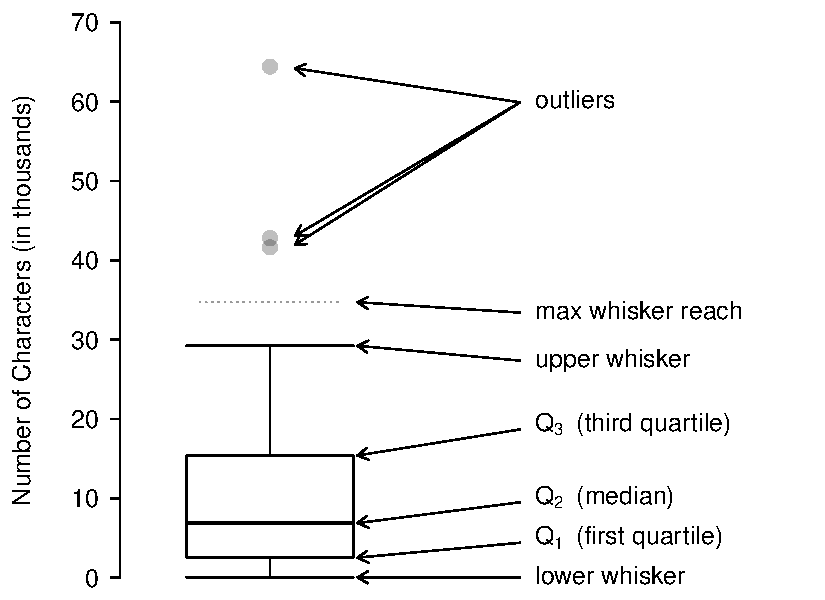
\includegraphics[width=0.9\mycaptionwidth]{ch_summarizing_data/figures/boxPlotLayoutNumVar/boxPlotLayoutNumVar}}
\caption{A labeled box plot for the number of characters in 50 emails. The median (6,890) splits the data into the bottom 50\% and the top 50\%.  Explore dozens of boxplots with histograms using American Community Survey data on Tableau Public~\tableauhref{tableau-boxplotschoose}.}
  % \caption{A vertical dot plot next to a labeled box plot for the number of characters in 50 emails. The median (6,890), splits the data into the bottom 50\% and the top 50\%, marked in the dot plot by horizontal dashes and open circles, respectively.}
   \label{boxPlotLayoutNumVar}
\end{figure}

The five summary statistics used in a box plot are known as the \term{five-number summary}, which consists of the minimum, the maximum, and the three quartiles ($Q_1$, $Q_2$, $Q_3$) of the data set being studied.

$Q_2$\index{quantile 2@Q$_2$} represents the \term{second quartile}, which is equivalent to the 50th percentile (i.e. the median). Previously, we saw that Q$_2$ (the median) for the \data{email50} data set was the average of the two middle values: $\frac{\text{6,768} + \text{7,012}}{2} = \text{6,890}$.

$Q_1$\index{quantile 1@Q$_1$} represents the \term{first quartile}, which is the 25th percentile, and is the median of the smaller half of the data set. There are 25 values in the lower half of the data set, so $Q_1$ is the middle value: 2,454 characters. $Q_3$\index{quantile 3@$Q_3$} represents the \term{third quartile}, or 75th percentile, and is the median of the larger half of the data set: 15,829 characters.

We calculate the variability in the data using the range of the middle 50\% of the data: $Q_3 - Q_1 = \text{13,375}$. This quantity is called the \termsub{interquartile range}{interquartile range (IQR)} (IQR, for short). It, like the standard deviation, is a measure of \indexthis{variability}{variability} or \term{spread} in data. The more variable the data, the larger the standard deviation and~IQR tend to be.

\D{\newpage}

\begin{onebox}{Interquartile range (IQR)}
The IQR\index{interquartile range (IQR)} is the length of the box in a box plot. It is computed as
\begin{eqnarray*}
IQR = Q_3 - Q_1
\end{eqnarray*}
where $Q_1$ and $Q_3$ are the $25^{th}$ and $75^{th}$ percentiles.\end{onebox}

\begin{onebox}{Outliers in the context of a box plot}
When in the context of a box plot, define an \term{outlier} as an \mbox{observation} that is more than $1.5 \times IQR$ above $Q_3$ or $1.5 \times IQR$ below $Q_1$. Such points are marked using a dot or asterisk in a box plot.\end{onebox}

To build a box plot, draw an axis (vertical or horizontal) and draw a scale. Draw a dark line denoting $Q_2$, the median. Next, draw a line at $Q_1$ and at $Q_3$. Connect the $Q_1$ and $Q_3$ lines to form a rectangle. The width of the rectangle corresponds to the IQR and the middle 50\% of the data is in this interval.

Extending out from the rectangle, the \term{whiskers} attempt to capture all of the data remaining outside of the box, except outliers. In Figure~\ref{boxPlotLayoutNumVar}, the upper whisker does not extend to the last three points, which are beyond $Q_3 + 1.5\times IQR$ and are outliers, so it extends only to the last point below this limit.\footnote{You might wonder, isn't the choice of $1.5 \times IQR$ for defining an outlier arbitrary? It is! In practical data analyses, we tend to avoid a strict definition since what is an unusual observation is highly dependent on the context of the data.} The lower whisker stops at the lowest value, 33, since there are no additional data to reach. Outliers are each marked with a dot or asterisk. In a sense, the box is like the body of the box plot and the whiskers are like its arms trying to reach the rest of the data.

\D{\newpage}

\begin{examplewrap}
\begin{nexample}{Compare the box plot to the graphs previously discussed: stem-and-leaf plot, dot plot, frequency and relative frequency histogram. What can we learn more easily from a box plot? What can we learn more easily from the other graphs?}
It is easier to immediately identify the quartiles from a box plot. The box plot also more prominently highlights outliers. However, a box plot, unlike the other graphs, does not show the \emph{distribution} of the data. For example, we cannot generally identify modes using a box plot.
\end{nexample}
\end{examplewrap}

\begin{examplewrap}
\begin{nexample}
{Is it possible to identify skew from the box plot?} Yes. Looking at the lower and upper whiskers of this box plot, we see that the lower 25\% of the data is squished into a shorter distance than the upper 25\% of the data, implying that there is greater density in the low values and a tail trailing to the upper values. This box plot is right skewed.
\end{nexample}
\end{examplewrap}

\begin{exercisewrap}
\begin{nexercise}
True or false: there is more data between the median and $Q_3$ than between $Q_1$ and the median.\footnotemark
\end{nexercise}
\end{exercisewrap}
\footnotetext{False. Since $Q_1$ is the 25th percentile and the median is the 50th percentile, 25\% of the data fall between $Q_1$ and the median. Similarly, 25\% of the data fall between $Q_2$ and the median. The distance between the median and $Q_3$ is larger because that 25\% of the data is more spread out.}

\begin{examplewrap}
\begin{nexample}
{Consider the following ordered data set.
\begin{center}
\begin{tabular}{ccc ccc ccc}
5 & 5 & 9 & 10 & 15 & 16 & 20 & 30 & 80 
\end{tabular}
\end{center}
Find the 5 number summary and identify how small or large a value would need to be to be considered an outlier.  Are there any outliers in this data set?}
There are nine numbers in this data set.  Because $n$ is odd, the median is the middle number: 15.  When finding $Q_1$, we find the median of the lower half of the data, which in this case includes 4 numbers (we do not include the 15 as belonging to either half of the data set).  $Q_1$ then is the average of 5 and 9, which is $Q_1 = 7$, and $Q_3$ is the average of 20 and 30, so $Q_3 = 25$.  The min is 5 and the max is 80.  To see how small a number needs to be to be an outlier on the low end we do:
\begin{align*}
Q_1 - 1.5 \times IQR
	&= Q_1 - 1.5 \times (Q_3 - Q_1) \\
	& = 7 - 1.5 \times (35 - 7) \\
	& = -35
\end{align*}
On the high end we need:
\begin{align*}
Q_3 + 1.5 \times IQR
	& = Q_3 + 1.5 \times (Q_3-Q_1) \\
	& = 35 + 1.5 \times (35 - 7) \\
	& = 77
\end{align*}
There are no numbers less than -41, so there are no outliers on the low end. The observation at 80 is greater than 77, so 80 is an outlier on the high end.
\end{nexample}
\end{examplewrap}

%\Comment{TODO(David)  create another box plot using different data set}
%\Comment{TODO(Leah) redo exercise}

%\Cut{
%\begin{exercisewrap}
%\begin{nexercise}
%Using Figure~\ref{boxPlotLayoutNumVar}, estimate the following values for \var{num\_\hspace{0.3mm}char} in the \data{email50} data set: (a) $Q_1$, (b) $Q_3$, and (c) IQR.\footnote{These visual estimates will vary a little from one person to the next: $Q_1=$ 3,000, $Q_3=$ 15,000, $\text{IQR}=Q_3 - Q_1 = $ 12,000. (The true values: $Q_1=$ 2,536, $Q_3=$ 15,411, $\text{IQR} = $ 12,875.)}
%\end{nexercise}
%\end{exercisewrap}
%}


%%


\D{\newpage}

\subsection{Calculator/Desmos: summarizing 1-variable statistics}
\label{summarizedata}

One can use a handheld calculator or online software such as Desmos to calculate summary statistics.  More advanced statistical software packages include R (in which most of the graphs in this text were made), Python, SAS, and STATA.

\begin{figure}[h]
   \centering
     \oiRedirect{textbook-desmos-1varstats}{ 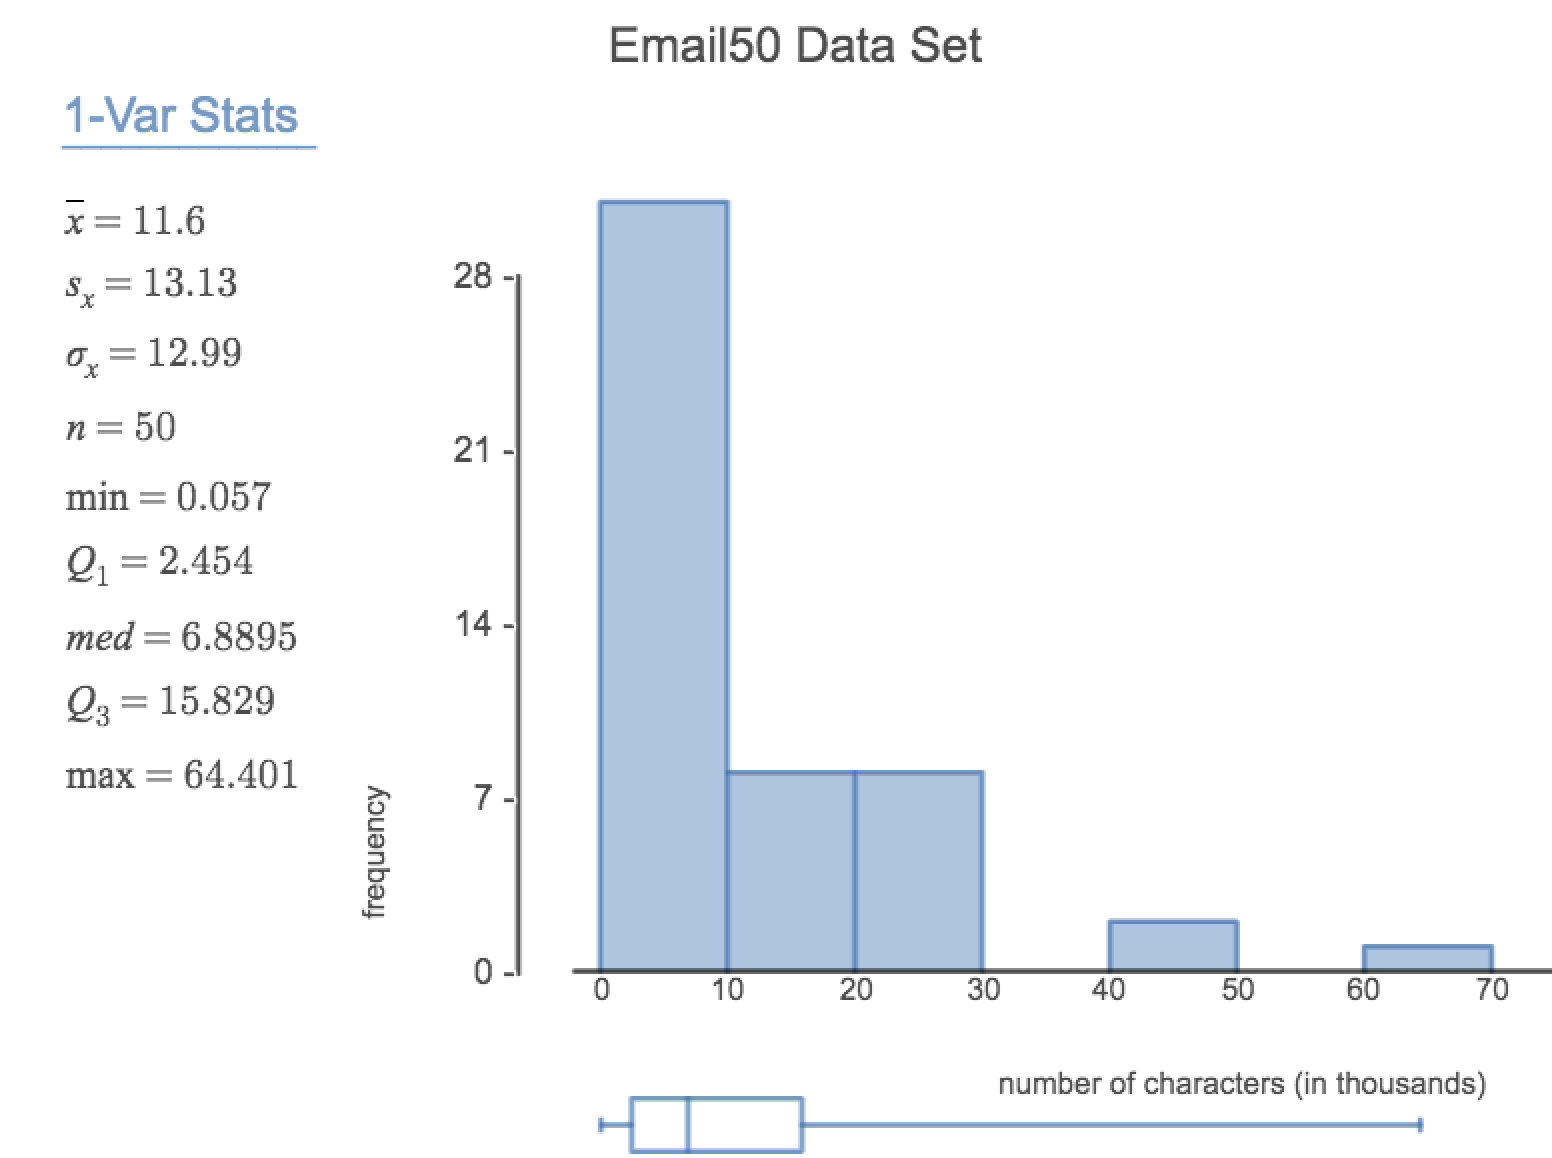
\includegraphics[width=0.85\textwidth]{ch_summarizing_data/figures/email50Desmos/email50Desmos}}
\caption{Use this \oiRedirect{textbook-desmos-1varstats}{1-Var Stats calculator} (\small{openintro.org/ahss/desmos}) to graph and find summary statistics for a single variable in Desmos, as shown in the figure.}
   \label{desmos1VarStats}
\end{figure}

\begin{onebox}{\videohref{ti84_entering_data} TI-83/84: Entering data}
The first step in summarizing data or making a graph is to  enter the data set into a list. Use \calcbutton{STAT}, \calctext{Edit}.
\begin{enumerate}
\setlength{\itemsep}{0mm}
\item Press \calcbutton{STAT}.
\item Choose \calctext{1:Edit}.
\item Enter data into \calctext{L1} or another list.
\end{enumerate}
\end{onebox}


\begin{onebox}{\videohref{casio_1_var_stats_and_box_plot} Casio fx-9750GII: Entering data}
\begin{enumerate}
\setlength{\itemsep}{0mm}
\item Navigate to \calctext{STAT} (\calcbutton{MENU} button, then hit the \calcbutton{2} button or select \calctext{STAT}).
\item Optional: use the left or right arrows to select a particular list.
\item Enter each numerical value and hit \calcbutton{EXE}.
\end{enumerate}
\end{onebox}

\begin{onebox}{\videohref{ti84_calculating_summary_statistics} TI-84: Calculating Summary Statistics}
\label{summstat}
Use the \calcbutton{STAT}, \calctext{CALC}, \calctext{1-Var Stats} command to find summary statistics such as mean, standard deviation, and quartiles.
\begin{enumerate}
\setlength{\itemsep}{0mm}
\item Enter the data as described previously.
\item Press \calcbutton{STAT}.
\item Right arrow to \calctext{CALC}.
\item Choose \calctext{1:1-Var Stats}.
\item Enter \calctext{L1} (i.e. \calcbutton{2ND} \calcbutton{1}) for List. If the data is in a list other than \calctext{L1}, type the name of that list.
\item Leave \calctext{FreqList} blank.
\item Choose \calctext{Calculate} and hit \calcbutton{ENTER}.
\end{enumerate}
TI-83: Do steps 1-4, then type \calctext{L1} (i.e. \calcbutton{2nd} \calcbutton{1}) or the list's name and hit \calcbutton{ENTER}.
\end{onebox}

Calculating the summary statistics will return the following information. It will be necessary to hit the down arrow to see all of the summary statistics.

\begin{center}
\begin{tabular}{ll l ll}
$\calctextmath{\bar{\text{x}}}$ & Mean &\quad&
	\calctext{n} & Sample size or \# of data points \\
$\calctextmath{\Sigma x}$ & Sum of all the data values &&
	\calctext{minX} & Minimum \\
$\calctextmath{\Sigma x^2}$ & Sum of all the squared data values &&
	$\calctextmath{Q_1}$ & First quartile\\
$\calctextmath{Sx}$ & Sample standard deviation &&
	\calctext{Med} & Median \\
$\calctextmath{\sigma x}$ & Population standard deviation &&
	\calctext{maxX} & Maximum 
\end{tabular}
\end{center}

\begin{onebox}{\videohref{ti84_box_plot} TI-83/84:  Drawing a box plot}
\label{boxplot}
\begin{enumerate}
\setlength{\itemsep}{0mm}
\item Enter the data to be graphed as described previously.
\item Hit \calcbutton{2ND} \calcbutton{Y=} (i.e. \calctext{STAT PLOT}).
\item Hit \calcbutton{ENTER} (to choose the first plot).
\item Hit \calcbutton{ENTER} to choose \calctext{ON}.
\item Down arrow and then right arrow three times to select box plot with outliers.
\item Down arrow again and make \calctext{Xlist:}~\calctext{L1} and \calctext{Freq:}~\calctext{1}.
\item Choose \calctext{ZOOM} and then \calctext{9:ZoomStat} to get a good viewing window.
\end{enumerate}
\end{onebox}

\begin{onebox}{\videohref{casio_1_var_stats_and_box_plot} Casio fx-9750GII: Drawing a box plot and 1-variable statistics}
\begin{enumerate}
\setlength{\itemsep}{0mm}
\item Navigate to \calctext{STAT} (\calcbutton{MENU}, then hit \calcbutton{2}) and enter the data into a list.
\item Go to \calctext{GRPH} (\calcbutton{F1}).
\item Next go to \calctext{SET} (\calcbutton{F6}) to set the graphing parameters.
\item To use the 2nd or 3rd graph instead of \calctext{GPH1}, select \calcbutton{F2} or \calcbutton{F3}.
\item Move down to \calctext{Graph Type} and select the $\calctextmath{\triangleright}$ (\calcbutton{F6}) option to see more graphing options, then select \calctext{Box} (\calcbutton{F2}).
\item If \calctext{XList} does not show the list where you entered the data, hit \calctext{LIST} (\calcbutton{F1}) and enter the correct list number.
\item Leave \calctext{Frequency} at \calctext{1}.
\item For \calctext{Outliers}, choose \calctext{On} (\calcbutton{F1}).
\item Hit \calcbutton{EXE} and then choose the graph where you set the parameters \calcbutton{F1} (most common), \calcbutton{F2}, or \calcbutton{F3}.
\item If desired, explore 1-variable statistics by selecting \calctext{1-Var} (\calcbutton{F1}).
\end{enumerate}
\end{onebox}

\begin{examplewrap}
\begin{nexample}{Enter the following 10 data points into a calculator or into this \oiRedirect{textbook-desmos-1varstatsdiscrete}{Desmos 1-Var Stats calculator} \mbox{(\small{openintro.org/ahss/desmos}):}
\begin{center}
{5, 8, 1, 19, 3, 1, 11, 18, 20, 5}
\end{center}
Find the summary statistics and make a box plot of the data.}
The summary statistics should be $\calctextmath{\bar{x}} = 9.1$, $\calctextmath{Sx} = 7.48$, $\calctextmath{Q1} = 3$, etc. The box plot should be as follows.
\begin{center}
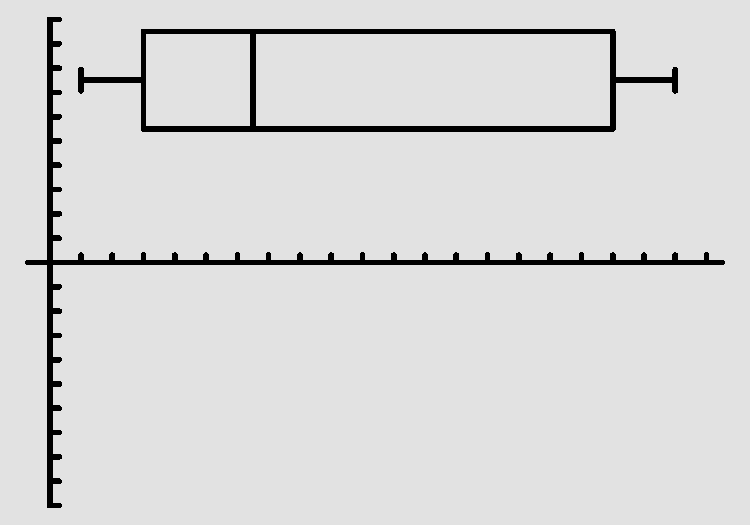
\includegraphics[width=0.48\textwidth]{ch_summarizing_data/figures/TI83_box_plot_A/TI83_box_plot_A} 
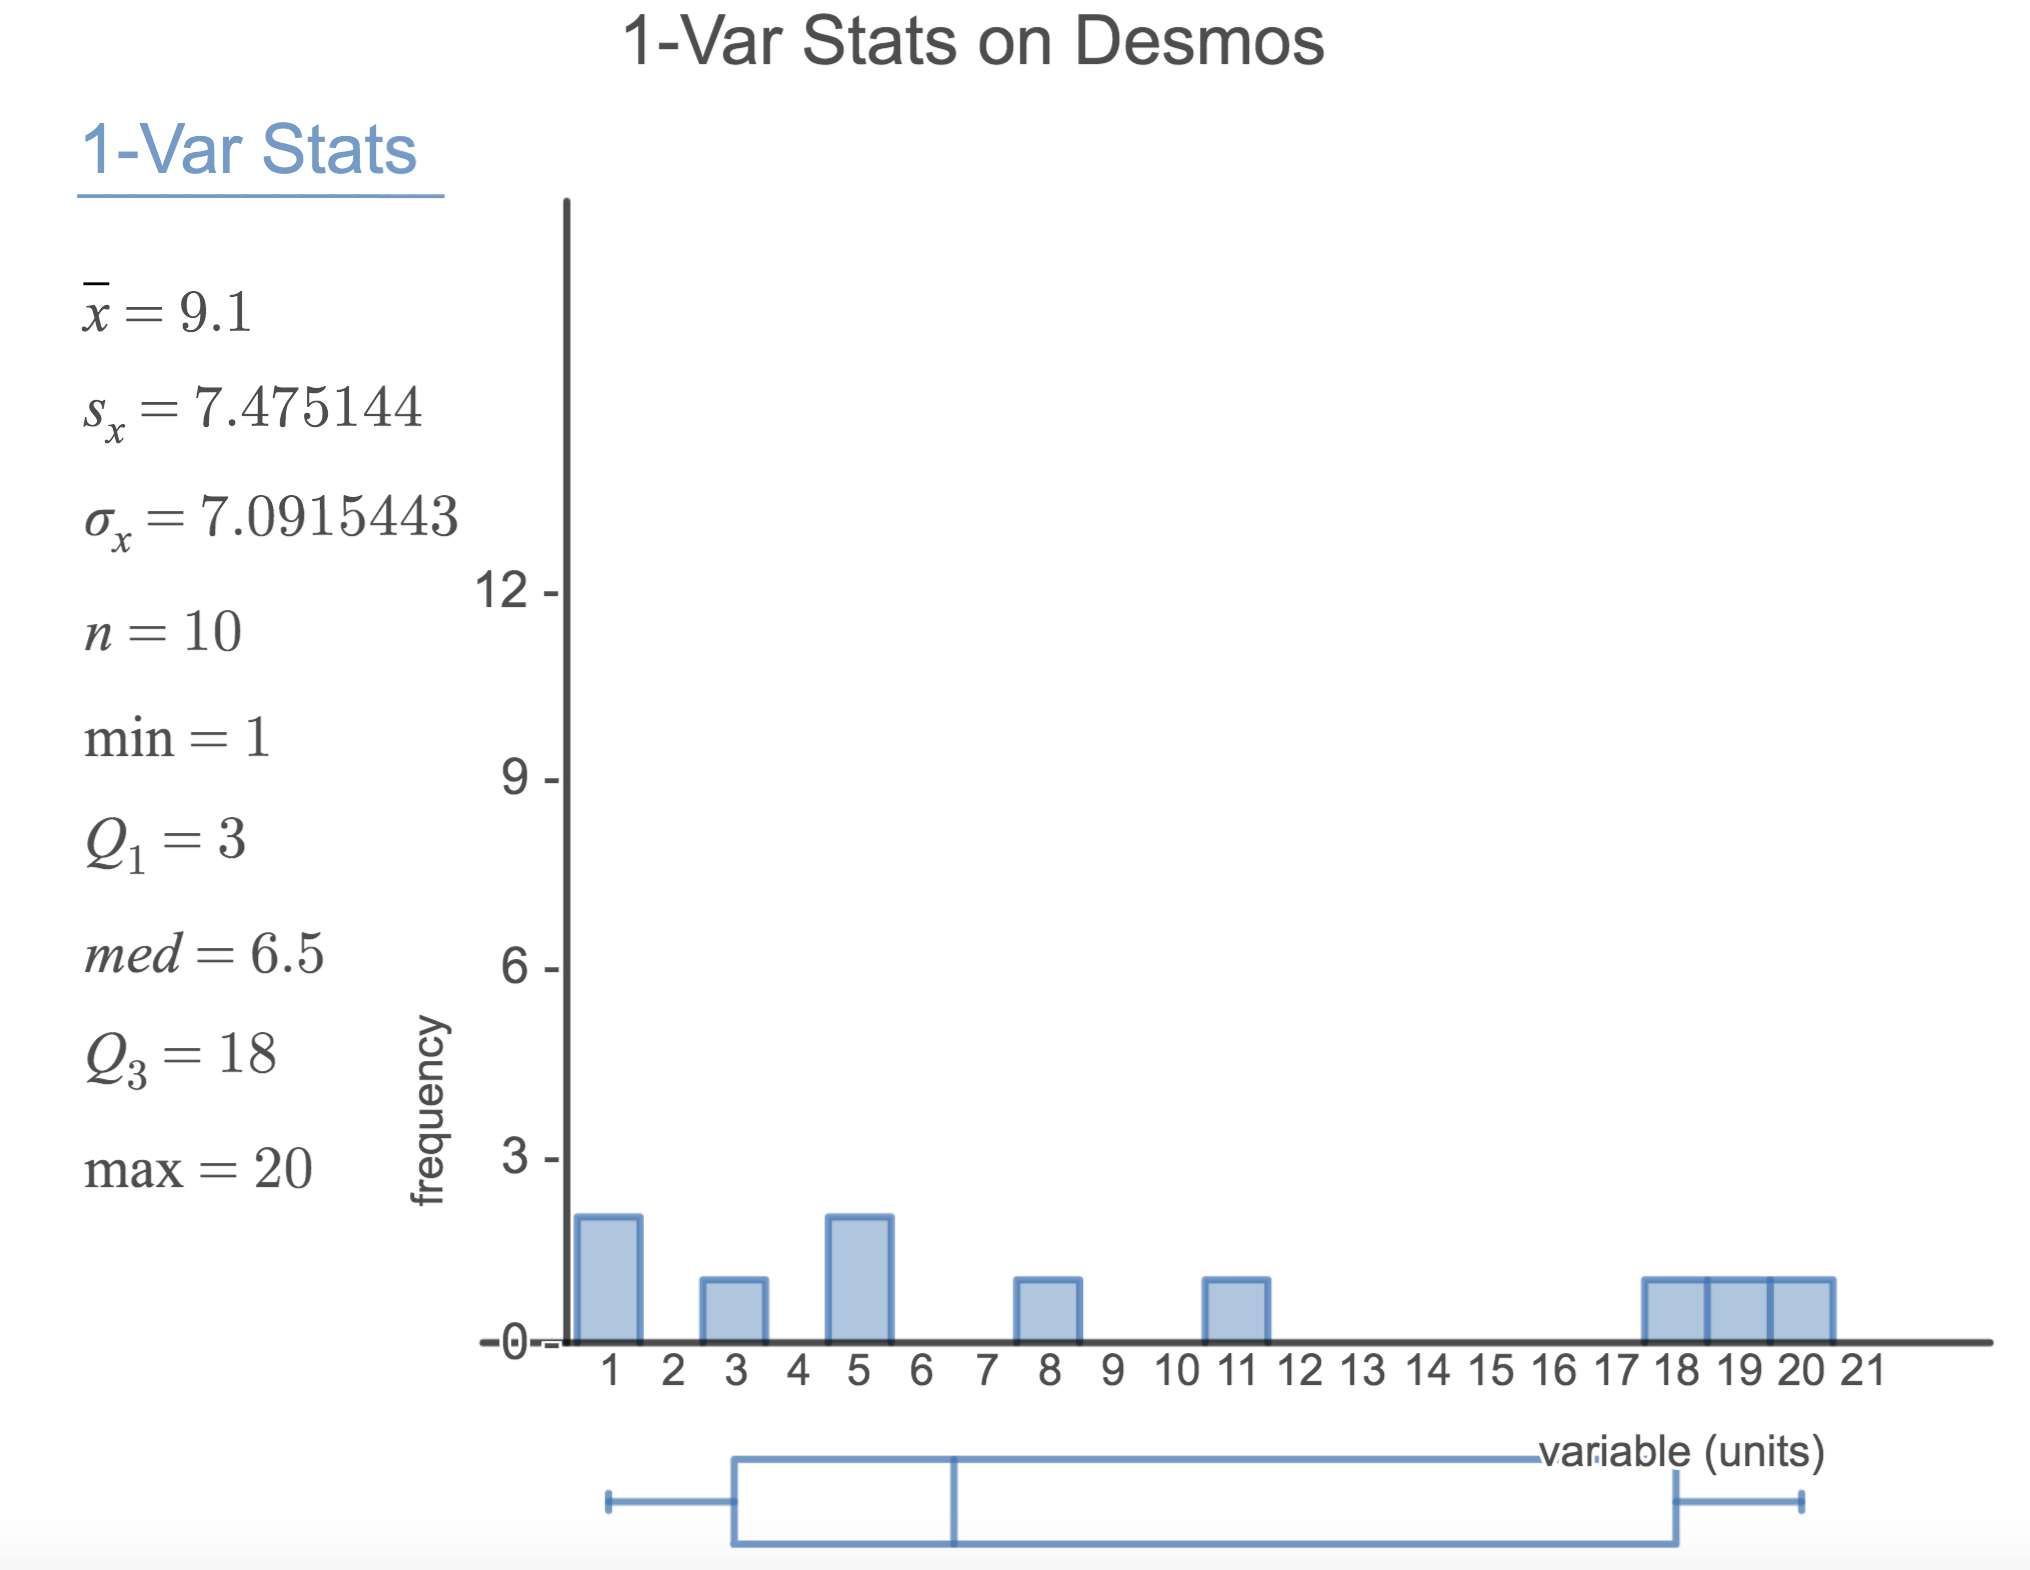
\includegraphics[width=0.48\textwidth]{ch_summarizing_data/figures/TI83_box_plot_A/1VarStatsDesmos}
\end{center}
\end{nexample}
\end{examplewrap}


\begin{onebox}{TI-83/84: What to do if you cannot find {L1} or another list}
Restore lists \calctext{L1}-\calctext{L6} using the following steps:
\begin{enumerate}
\setlength{\itemsep}{0mm}
\item Press \calcbutton{STAT}.
\item Choose \calctext{5:SetUpEditor}.
\item Hit \calcbutton{ENTER}.
\end{enumerate}\end{onebox}

\newpage
\begin{onebox}{\videohref{casio_1_var_stats_and_box_plot} Casio fx-9750GII: Deleting a data list}
\begin{enumerate}
\setlength{\itemsep}{0mm}
\item Navigate to \calctext{STAT} (\calcbutton{MENU}, then hit \calcbutton{2}).
\item Use the arrow buttons to navigate to the list you would like to delete.
\item Select $\calctextmath{\triangleright}$ (\calcbutton{F6}) to see more options.
\item Select \calctext{DEL-A} (\calcbutton{F4}) and then \calcbutton{F1} to confirm.
\end{enumerate}
\end{onebox}


%%
\subsection{Outliers and robust statistics}

\begin{onebox}{Rules of thumb for identifying outliers}
There are two rules of thumb for identifying outliers:
\begin{itemize}
\setlength{\itemsep}{0mm}
\item More than 1.5$\times$ IQR below $Q_1$ or above $Q_3$
\item More than 2 standard deviations above or below the mean.
\end{itemize}
Both are important for the AP exam. In practice, consider these to be only rough guidelines.\end{onebox}

\begin{exercisewrap}
\begin{nexercise}For the \data{email50} data set,$Q_1=$ 2,536 and $Q_3=15,411$. $\bar{x}$ = 11,600  and $s$ = 13,130. What values would be considered an outlier on the low end using each rule?\footnotemark
\end{nexercise}
\end{exercisewrap}
\footnotetext{ $Q_1 - 1.5\times IQR = 2536 - 1.5 \times (15411 - 2536) = -16,749.5$, so values less than -16,749.5 would be considered an outlier using the first rule of thumb. Using the second rule of thumb, a value less than $\bar{x} - 2\times s = 11,600 - 2 \times 13,130 = -14,660$ would be considered an outlier. Note tht these are just rules of thumb and yield different values.}


\begin{exercisewrap}
\begin{nexercise} Because there are no negative values in this data set, there can be no outliers on the low end. What does the fact that there are outliers on the high end but not on the low end suggestion?\footnotemark
\end{nexercise}
\end{exercisewrap}
\footnotetext{It suggests that the distribution has a right hand tail, that~is, that it is right skewed.}

How are the \indexthis{sample statistics}{sample statistic} of the \data{num\_\hspace{0.3mm}char} data set affected by the observation, 64,401? What would have happened if this email wasn't observed? What would happen to these \indexthis{summary statistics}{summary statistic} if the observation at 64,401 had been even larger, say 150,000? These scenarios are plotted alongside the original data in Figure~\ref{email50NumCharDotPlotRobustEx}, and sample statistics are computed under each scenario in Figure~\ref{robustOrNotTable}.

\begin{figure}[ht]
\centering
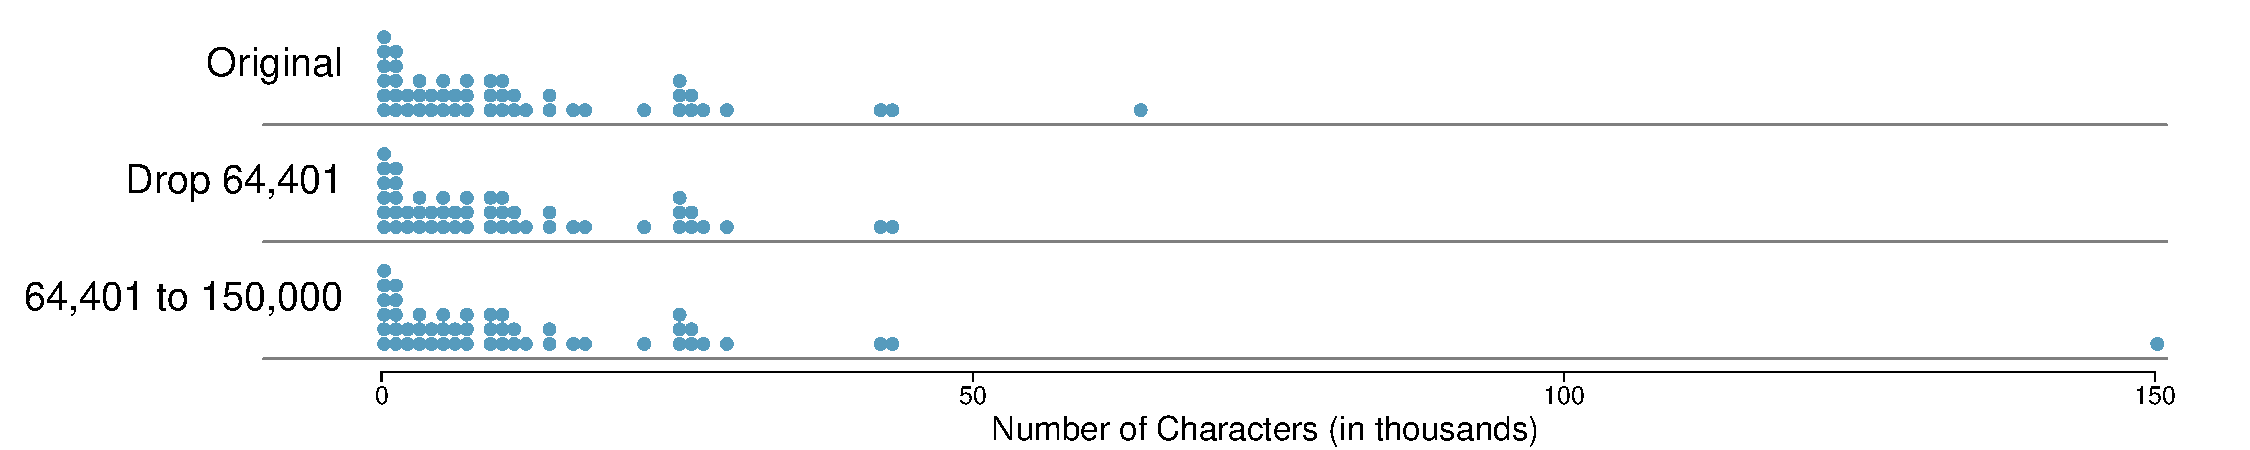
\includegraphics[width=\textwidth]{ch_summarizing_data/figures/emailCharactersDotPlot/email50NumCharDotPlotRobustEx}
\caption{Dot plots of the original character count data and two modified data sets.}
\label{email50NumCharDotPlotRobustEx}
\end{figure}

\D{\newpage}

\begin{figure}[ht]
\centering
\begin{tabular}{l c cc c cc}
  \hline
& \hspace{0mm} & \multicolumn{2}{c}{\bf robust} & \hspace{2mm} & \multicolumn{2}{c}{\bf not robust} \\
scenario && median & IQR && $\bar{x}$ & $s$ \\
  \hline
original \var{num\_\hspace{0.3mm}char} data 	&& 6,890 & 12,875 && 11,600 & 13,130 \\
% library(openintro); data(email50); d <- email50$num_char; median(d); diff(quantile(d, c(0.25,0.75))); mean(d); sd(d)
drop 64,401 observation		&& 6,768 & 11,702 && 10,521 & 10,798 \\
% library(openintro); data(email50); d <- email50$num_char; d <- d[-which.max(d)]; median(d); diff(quantile(d, c(0.25,0.75))); mean(d); sd(d)
move 64,401 to 150,000		&& 6,890 & 12,875 && 13,310 & 22,434 \\
% library(openintro); data(email50); d <- email50$num_char; d[which.max(d)] <- 100000; median(d); diff(quantile(d, c(0.25,0.75))); mean(d); sd(d)
   \hline
\end{tabular}
\caption{A comparison of how the median, IQR, mean ($\bar{x}$), and standard deviation ($s$) change when extreme observations are present.}
\label{robustOrNotTable}
\end{figure}

\begin{exercisewrap}
\begin{nexercise} \label{numCharWhichIsMoreRobust}
(a) Which is more affected by extreme observations, the mean or median? Figure~\ref{robustOrNotTable} may be helpful. (b) Is the standard deviation or IQR more affected by extreme observations?\footnotemark
\end{nexercise}
\end{exercisewrap}
\footnotetext{(a) Mean is affected more. (b) Standard deviation is affected more. Complete explanations are provided in the material following Guided Practice~\ref{numCharWhichIsMoreRobust}.}

The median and IQR are called \term{robust estimates} because extreme observations have little effect on their values. The mean and standard deviation are much more affected by changes in extreme observations.

\begin{examplewrap}
\begin{nexample}{The median and IQR do not change much under the three scenarios in Figure~\ref{robustOrNotTable}. Why might this be the case?}
Since there are no large gaps between observations around the three quartiles, adding, deleting, or changing one value, no matter how extreme that value, will have little effect on their values.
\end{nexample}
\end{examplewrap}

\begin{exercisewrap}
\begin{nexercise}
The distribution of vehicle prices tends to be right skewed, with a few luxury and sports cars lingering out into the right tail. If you were searching for a new car and cared about price, should you be more interested in the mean or median price of vehicles sold, assuming you are in the market for a regular car?\footnotemark\end{nexercise}
\end{exercisewrap}
\footnotetext{Buyers of a ``regular car'' should be concerned about the median price. High-end car sales can drastically inflate the mean price while the median will be more robust to the influence of those sales.}

%%
\subsection{Linear transformations of data}
\label{linearTransformationOfData}

\begin{examplewrap}
\begin{nexample}{Begin with the following list:  {1, 1, 5, 5}. Multiply all of the numbers by 10. What happens to the mean? What happens to the standard deviation? How do these compare to the mean and the standard deviation of the original list?}
The original list has a mean of 3 and a standard deviation of 2. The new list: {10, 10, 50, 50} has a mean of 30 with a standard deviation of 20. Because all of the values were multiplied by 10, both the mean and the standard deviation were multiplied by~10.~\footnotemark
\end{nexample}
\end{examplewrap}
\footnotetext{Here, the population standard deviation was used in the calculation. These properties can be proven mathematically using properties of sigma (summation).}

\D{\newpage}

\begin{examplewrap}
\begin{nexample}{Start with the following list:  {1, 1, 5, 5}. Multiply all of the numbers by \mbox{-0.5}. What happens to the mean? What happens to the standard deviation? How do these compare to the mean and the standard deviation of the original list?}
The new list: {-0.5, -0.5, -2.5, -2.5} has a mean of -1.5 with a standard deviation of~1. Because all of the values were multiplied by~\mbox{-0.5}, the mean was multiplied by~\mbox{-0.5}. Multiplying all of the values by a negative flipped the sign of numbers, which affects the location of the center, but not the spread. Multiplying all of the values by \mbox{-0.5} multiplied the standard deviation by +0.5 since the standard deviation cannot be negative.
\end{nexample}
\end{examplewrap}

\begin{examplewrap}
\begin{nexample}{Again, start with the following list: {1, 1, 5, 5}. Add 100 to every entry. How do the new mean and standard deviation compare to the original mean and standard deviation?}
The new list is: {101, 101, 105, 105}. The new mean of 103 is 100 greater than the original mean of 3. The new standard deviation of 2 is the \emph{same} as the original standard deviation of 2. Adding a constant to every entry shifted the values, but did not stretch them.
\end{nexample}
\end{examplewrap}

Suppose that a researcher is looking at a list of 500 temperatures recorded in Celsius~(C). The mean of the temperatures listed is given as 27\degree C with a standard deviation of 3\degree C. Because she is not familiar with the Celsius scale, she would like to convert these summary statistics into Fahrenheit~(F). To convert from Celsius to Fahrenheit, we use the following conversion:
\begin{align*}
x_{_F} = \frac{9}{5}x_{_C} + 32
\end{align*}
Fortunately, she does not need to convert each of the 500 temperatures to Fahrenheit and then recalculate the mean and the standard deviation. The unit conversion above is a linear transformation of the following form, where $a=9/5$ and $b=32$:
\begin{align*}
aX + b
\end{align*}
Using the examples as a guide, we can solve this temperature-conversion problem. The mean was 27\degree C and the standard deviation was 3\degree C. To convert to Fahrenheit, we multiply all of the values by $9/5$, which multiplies both the mean and the standard deviation by $9/5$. Then we add 32 to all of the values which adds 32 to the mean but does not change the standard deviation further.
\begin{align*}
\bar{x}_{F} &= \frac{9}{5}\bar{x}_{C} + 32 & \sigma_{F} &= \frac{9}{5}\sigma_{C} \\
&= \frac{5}{9}(27)+ 32 & &=\frac{9}{5}(3) \\
&=80.6 &  &=5.4
\end{align*}

\begin{figure}[h]
   \centering
   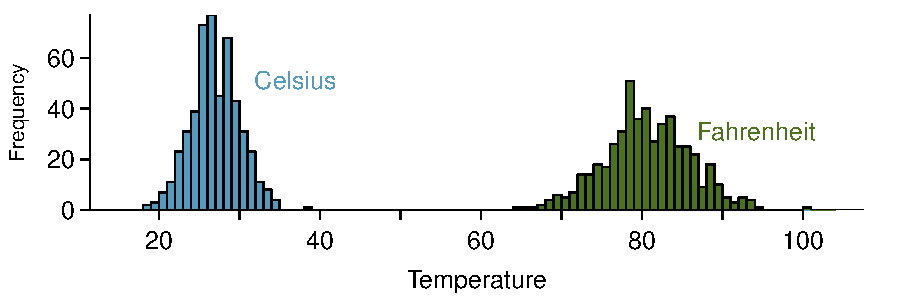
\includegraphics[width=0.9\textwidth]{ch_summarizing_data/figures/CToF_ConversionFigure/CToF_ConversionFigure}
   \caption{500 temperatures shown in both Celsius and \mbox{Fahrenheit.}}
   \label{CToF_ConversionFigure}
\end{figure}

%\Comment{TODO(David) THIS WOULD BE NICE add picture}

\begin{onebox}{Adding shifts the values, multiplying stretches or contracts them}
Adding a constant to every value in a data set shifts the mean but does not affect the standard deviation. Multiplying the values in a data set by a constant will change the mean and the standard deviation by the same multiple, except that the standard deviation will always remain positive.\end{onebox}

\begin{examplewrap}
\begin{nexample}{Consider the temperature example. How would converting from Celsuis to Fahrenheit affect the median? The IQR?}
The median is affected in the same way as the mean and the IQR is affected in the same way as the standard deviation. To get the new median, multiply the old median by $9/5$ and add 32. The IQR is computed by subtracting $Q_1$ from $Q_3$. While $Q_1$ and $Q_3$ are each affected in the same way as the median, the additional 32 added to each will cancel when we take $Q_3 - Q_1$. That is, the IQR will be increase by a factor of $9/5$ but will be unaffected by the addition of~32.

For a more mathematical explanation of the IQR calculation, see the footnote.\footnote{new IQR = $\left(\frac{9}{5} Q_3 + 32\right) - \left(\frac{9}{5} Q_1 + 32\right) = \frac{9}{5} \left(Q_3 - Q_1\right) = \frac{9}{5} \times \text{(old IQR)}$.}
\end{nexample}
\end{examplewrap}

%%
\subsection{Comparing numerical data across groups}
\label{comparingAcrossGroups}

\index{data!county|(}



Some of the more interesting investigations can be considered by examining numerical data across groups. The methods required here aren't really new. All that is required is to make a numerical plot for each group. To make a direct comparison between two groups, create a pair of dot plots or a pair of histograms drawn using the same scales. It is also common to use back-to-back stem-and-leaf plots, parallel box plots, and hollow histograms, the three of which are explored here.

We will take a look again at the \data{county} data set
and compare the median household income for counties that
gained population from 2010 to 2017 versus counties that
had no gain.
While we might like to make a causal connection here,
remember that these are observational data and so such
an interpretation would be, at best, half-baked.

\newcommand{\numcountieswithgains}{1454}
\newcommand{\numcountieswithgainsC}{1,454}
\newcommand{\numcountieswithoutgains}{1672}
\newcommand{\numcountieswithoutgainsC}{1,672}

There were \numcountieswithgainsC{} counties where
the population increased from 2010 to 2017, and there
were \numcountieswithoutgainsC{} counties with no gain
(all but one were a loss).
A~random sample of 100 counties from the first group and
50 from the second group are shown in
Figure~\ref{countyIncomeSplitByPopGainTable}
to give a better sense of some of the raw median
income data.

\newcommand{\npgpad}[1]{\hspace{2mm}#1\hspace{1.5mm}\ }
\begin{figure}
\begin{center}
\begin{tabular}{ ccc ccc c ccc }
\multicolumn{10}{c}{\bf Median Income for 150 Counties,
    in \$1000s} \\
\hline
\vspace{-2mm} \\
\multicolumn{6}{c}{\bf Population Gain} &\hspace{5mm}\ &
    \multicolumn{3}{c}{\bf No Population Gain} \\ 
  \cline{1-6} \cline{8-10}
38.2 & 43.6 & 42.2 & 61.5 & 51.1 & 45.7 &&
    \npgpad{48.3} & \npgpad{60.3} & \npgpad{50.7} \\
44.6 & 51.8 & 40.7 & 48.1 & 56.4 & 41.9 && 39.3 & 40.4 & 40.3 \\
40.6 & 63.3 & 52.1 & 60.3 & 49.8 & 51.7 && 57 & 47.2 & 45.9 \\
51.1 & 34.1 & 45.5 & 52.8 & 49.1 & 51 && 42.3 & 41.5 & 46.1 \\
80.8 & 46.3 & 82.2 & 43.6 & 39.7 & 49.4 && 44.9 & 51.7 & 46.4 \\
75.2 & 40.6 & 46.3 & 62.4 & 44.1 & 51.3 && 29.1 & 51.8 & 50.5 \\
51.9 & 34.7 & 54 & 42.9 & 52.2 & 45.1 && 27 & 30.9 & 34.9 \\
61 & 51.4 & 56.5 & 62 & 46 & 46.4 && 40.7 & 51.8 & 61.1 \\
53.8 & 57.6 & 69.2 & 48.4 & 40.5 & 48.6 && 43.4 & 34.7 & 45.7 \\
53.1 & 54.6 & 55 & 46.4 & 39.9 & 56.7 && 33.1 & 21 & 37 \\
63 & 49.1 & 57.2 & 44.1 & 50 & 38.9 && 52 & 31.9 & 45.7 \\
46.6 & 46.5 & 38.9 & 50.9 & 56 & 34.6 && 56.3 & 38.7 & 45.7 \\
74.2 & 63 & 49.6 & 53.7 & 77.5 & 60 && 56.2 & 43 & 21.7 \\
63.2 & 47.6 & 55.9 & 39.1 & 57.8 & 42.6 && 44.5 & 34.5 & 48.9 \\
50.4 & 49 & 45.6 & 39 & 38.8 & 37.1 && 50.9 & 42.1 & 43.2 \\
57.2 & 44.7 & 71.7 & 35.3 & 100.2 &  && 35.4 & 41.3 & 33.6 \\
42.6 & 55.5 & 38.6 & 52.7 & 63 &  && 43.4 & 56.5 &  \\
\cline{1-6} \cline{8-10}
\end{tabular}
\caption{In this table, median household income (in \$1000s)
    from a random sample of 100 counties that had population
    gains are shown on the left.
    Median incomes from a random sample of 50 counties that
    had no population gain are shown on the right.}
\label{countyIncomeSplitByPopGainTable}
\end{center}
\end{figure}

\begin{figure}
\begin{verbatim}
                         Population: Gain           Population: No Gain

                                            | 2 |12                          
                                            | 2 |79                          
                                           4| 3 |1234                    
                                 99999987555| 3 |5555799                 
                             444433322111000| 4 |00111223333              
                       999998887666666665555| 4 |55666666789                
                       444333222221111110000| 5 |1112222                    
                                887776666555| 5 |6677                       
                                 33333222100| 6 |01                          
                                           9| 6 |                             
                                          42| 7 |                             
                                          85| 7 |                             
                                          21| 8 |    
               
                       Legend: 2 |1 = 21,000 median income
\end{verbatim}
\caption{Back-to-back stem-and-leaf plot for median income, split by whether the count had a population gain or no gain.}
\label{stemandleafincomepopgainloss}
\end{figure}

The \term{side-by-side box plot}
\index{box plot!side-by-side box plot}
is a traditional tool for comparing across groups.
An example is shown in the left panel of
Figure~\ref{countyIncomeSplitByPopGain},
where there are two box plots, one for each group,
placed into one plotting window and drawn on the same scale.

\begin{figure}
  \centering
\oiRedirect{tableau-medianincome-gainnogain-all}{
  \Figure{1.00}{countyIncomeSplitByPopGain}}
  \caption{Side-by-side box plot (left panel)
      and hollow histograms (right panel) for
      \var{med\us{}hh\us{}income},
      where the counties are split by whether or not there was a population gain from 2010 to 2017.  Explore this data set on Tableau Public~\tableauhref{tableau-medianincome-gainnogain-all}.}
  \label{countyIncomeSplitByPopGain}
\end{figure}

Another useful plotting method uses \termsub{hollow histograms}{hollow histogram} to compare numerical data across groups. These are just the outlines of histograms of each group put on the same plot, as shown in the right panel of Figure~\ref{countyIncomeSplitByPopGain}.

\begin{exercisewrap}
\begin{nexercise} \label{comparingPriceByTypeExercise}
Use the plots in Figure~\ref{countyIncomeSplitByPopGain}
to compare the incomes for counties across the two groups.
What do you notice about the approximate center of each group?
What do you notice about the variability between groups?
Is the shape relatively consistent between groups?
How many \emph{prominent} modes are there for each
group?\footnotemark{}
\end{nexercise}
\end{exercisewrap}
\footnotetext{Answers may vary a little.
  The counties with population gains tend to have higher
  income (median of about \$45,000) versus counties without
  a gain (median of about \$40,000).
  The variability is also slightly larger for the population
  gain group.
  This is evident in the IQR, which is about 50\% bigger
  in the \emph{gain} group.
  Both distributions show slight to moderate right
  skew\index{skew!example: slight to moderate}
  and are unimodal.
  The box plots indicate there are many observations
  far above the median in each group, though we should
  anticipate that many observations will fall beyond
  the whiskers when examining any data set that
  contain more than a couple hundred data points.}

\begin{onebox}{Comparing distributions}
When comparing distributions, compare them with respect to center, spread, and shape as well as any unusual observations. Such descriptions should be in context.\end{onebox}

\begin{exercisewrap}
\begin{nexercise}
What components of each plot in Figure~\ref{countyIncomeSplitByPopGain} do you find most useful?\footnotemark\end{nexercise}
\end{exercisewrap}
\footnotetext{Answers will vary. The parallel box plots are especially useful for comparing centers and spreads, while the hollow histograms are more useful for seeing distribution shape, skew, and groups of anomalies.}

\begin{exercisewrap}
\begin{nexercise}
Do these graphs tell us about any association between income for the two groups?\footnotemark
\end{nexercise}
\end{exercisewrap}
\footnotetext{No, to see association we require a scatterplot. Moreover, these data are not paired, so the discussion of association does not make sense here.}

Looking at an association is different than comparing distributions. When comparing distributions, we are interested in questions such as, ``Which distribution has a greater average?'' and ``How do the shapes of the distribution differ?'' The number of elements in each data set need not be the same (e.g. height of women and height of men). When we look at association, we are interested in whether there is a positive, negative, or no association between the variables. This requires two data sets of equal length that are essentially paired (e.g. height and weight of individuals).

\begin{onebox}{Comparing distributions versus looking at association}
We compare two distributions with respect to center, spread, and shape.  To compare the distributions visually, we use 2 single-variable graphs, such as two histograms, two dot plots, parallel box plots, or a back-to-back stem-and-leaf. When looking at association, we look for a positive, negative, or no relationship between the variables. To see association visually, we require a scatterplot.\end{onebox}


\index{data!email50|)}


%%
\subsection{Mapping data (special topic)}

\index{data!county|(}
\index{intensity map|(}

The \data{county} data set offers many numerical variables
that we could plot using dot plots, scatterplots,
or box plots, but these miss the true nature of the data.
Rather, when we encounter geographic data, we should create
an \term{intensity map}, where colors are used
to show higher and lower values of a variable.
Figures~\ref{countyIntensityMaps1}
and~\ref{countyIntensityMaps2} shows intensity maps for
poverty rate in percent (\var{poverty}),
unemployment rate (\var{unemployment\us{}rate}),
homeownership rate in percent (\var{homeownership}),
and median household income
(\var{median\us{}hh\us{}income}).
The color key indicates which colors correspond to which values.
The intensity maps are not generally very helpful
for getting precise values in any given county,
but they are very helpful for seeing geographic trends
and generating interesting research questions or hypotheses.

\begin{examplewrap}
\begin{nexample}{What interesting features are evident in the
    \var{poverty} and \var{unemployment\us{}rate}
    intensity maps?}
  Poverty rates are evidently higher in a few locations.
  Notably, the deep south shows higher poverty rates,
  as does much of Arizona and New Mexico.
  High poverty rates are evident in the Mississippi
  flood plains a little north of New Orleans and
  also in a large section of Kentucky.

  The unemployment rate follows similar trends,
  and we can see correspondence between the two
  variables. In fact, it makes sense for higher rates
  of unemployment to be closely related to poverty rates.
  One observation that stand out when comparing the two maps:
  the poverty rate is much higher than the unemployment
  rate, meaning while many people may be working,
  they are not making enough to break out of poverty.
\end{nexample}
\end{examplewrap}

\begin{exercisewrap}
\begin{nexercise}
What interesting features are evident in the
\var{median\us{}hh\us{}income} intensity map in
Figure~\ref{countyMedIncomeMap}?\footnotemark{}
\end{nexercise}
\end{exercisewrap}
\footnotetext{Note: answers will vary.
  There is some correspondence between high earning
  and metropolitan areas, where we can see darker spots
  (higher median household income),
  though there are several exceptions.
  You might look for large cities you are familiar with and
  try to spot them on the map as dark spots.}

\begin{figure}
  \centering
\oiRedirect{tableau-intensitymapsall}{
  \subfigure[]{
    \Figures{1.00}
        {countyIntensityMaps}
        {countyPovertyMap}
    \label{countyPovertyMap}
  }
  \subfigure[]{
    \Figures{1.00}
        {countyIntensityMaps}
        {countyUnemploymentRateMap}
    \label{countyUnemploymentRateMap}
  }}
  \caption{\subref{countyPovertyMap} Intensity map of
      poverty rate (percent).
      \subref{countyUnemploymentRateMap}~Intensity map of the
      unemployment rate (percent).  Explore dozens of intensity maps using American Community Survey data on Tableau Public~\tableauhref{tableau-intensitymapsall}.}
  \label{countyIntensityMaps1}
\end{figure}

\begin{figure}
  \centering
\oiRedirect{tableau-intensitymapsall}{
  \subfigure[]{
    \Figures{1.00}
        {countyIntensityMaps}
        {countyHomeownershipMap}
    \label{countyHomeownershipMap}
  }
  \subfigure[]{
    \Figures{1.00}
        {countyIntensityMaps}
        {countyMedIncomeMap}
    \label{countyMedIncomeMap}
  }}
  \caption{\subref{countyHomeownershipMap} Intensity map
      of homeownership rate (percent).
      \subref{countyMedIncomeMap}~Intensity map of median
      household income (\$1000s).  Explore dozens of intensity maps using American Community Survey data on Tableau Public~\tableauhref{tableau-intensitymapsall}.}
\label{countyIntensityMaps2}
\end{figure}

\index{intensity map|)}
\index{data!county|)}



\D{\newpage}

%%
\subsection*{Section summary}

\begin{itemize}
 \item In this section we looked at univariate summaries, including two measures of \term{center} and three measures of \term{spread}.  
\item When \term{summarizing} or \term{comparing distributions}, always comment on center, spread, and shape.  Also, mention outliers or gaps if applicable.  Put descriptions in \textit{context}, that is, identify the variable(s) being summarized by name and include relevant units.  Remember:  \textit{Center, Spread, and Shape!  In context!}
\item \termsub{Mean}{mean} and \term{median} are measures of center.  (A common mistake is to report \term{mode} as a measure of center. However, a mode can appear anywhere in a distribution.)  

\begin{itemize}
\item   The \term{mean} is the sum of all the observations divided by the
  number of observations, $n$. \\
  $\bar{x} = \frac{1}{n}\sum{x_{i}} = \frac{\sum{x_i}}{n}=\frac{x_1 + x_2 + ... + x_n}{n}$\\
  
\item In an ordered data set, the \term{median} is the middle number when $n$ is odd.  When $n$ is even, the median is the average of the two middle numbers. 

\end{itemize} 

\item Because large values exert more ``pull" on the mean, large values on the high end tend to increase the mean more than they increase the median.  In a \term{right skewed} distribution, therefore, the mean is greater than the median.  Analogously, in a \term{left skewed} distribution, the mean is less than the median.  Remember: \textit{The mean follows the tail!  The skew is the tail!}

\item \termsub{Standard deviation (SD)}{standard deviation} and \termsub{Interquartile range (IQR)}{interquartile range (IQR)} are measures of spread.  SD measures the typical spread from the mean, whereas IQR measures the spread of the middle 50\% of the data.
\begin{itemize}
\item To calculate the standard deviation, subtract the average from each value, square all those differences, add them up, divide by $n -1$, then take the square root.  Note:  The standard deviation is the square root of the variance. 

\item[]   $s_{\scriptscriptstyle{X}}
 = \sqrt{\frac{1}{n-1} \sum{(x_i -  \bar{x})^2}}$ 

\item The IQR is the difference between the third quartile $Q_3$ and the first quartile $Q_1$.

\item[] $IQR = Q_3 - Q_1$ 
\end{itemize}


\item \termsub{Range}{range} is also sometimes used as a measure of spread.  The range of a data set is defined as the difference between the maximum value and the minimum value, i.e. $max - min$.

\item \termsub{Outliers}{outlier} are observations that are extreme relative to the rest of the data.  Two rules of thumb for identifying observations as outliers are:
\begin{itemize}\vspace{-1mm}
\setlength{\itemsep}{0mm}
\item more than 2 standard deviations above or below the mean
\item more than $1.5 \times IQR$ below $Q_1$ or above $Q_3$
\end{itemize}
Note: These rules of thumb generally produce different cutoffs.
\item Mean and SD are sensitive to outliers.  Median and IQR are more robust and less sensitive to outliers.

\item The \term{empirical rule} states that for normal distributions, about 68\% of the data will be within one standard deviation of the mean, about 95\% will be within two standard deviations of the mean, and about 99.7\% will be within three standard deviations of the mean.
\item \termsub{Linear transformations of data}{linear transformations of data}.  Adding a constant to every value in a data set shifts the mean but does not affect the standard deviation. Multiplying the values in a data set by a constant will multiply the mean and the standard deviation by that constant, except that the standard deviation must always remain positive. 

\item \termsub{Box plots}{box plot} do not show the \textit{distribution} of a data set in the way that histograms do.
Rather, they provide a visual depiction of the \term{5-number summary}, which consists of: $min$, $Q_1$, $Q_2$, $Q_3$, $max$.
It is important to be able to identify the median, $IQR$, and direction of skew from a box plot.  


\end{itemize}


%%%%%%%%%%%Section Exercises
{\exercisesheader{}

% 7
\eoce{\qt{Smoking habits of UK residents, Part I\label{UKSmoking_amounts}} A survey was conducted to study the smoking habits of UK residents. The histograms below display the distributions of the number of cigarettes smoked on weekdays and weekends, and they exclude data from people who identified themselves as non-smokers. Describe the two distributions and compare them. \footfullcite{data:smoking}
\begin{center}
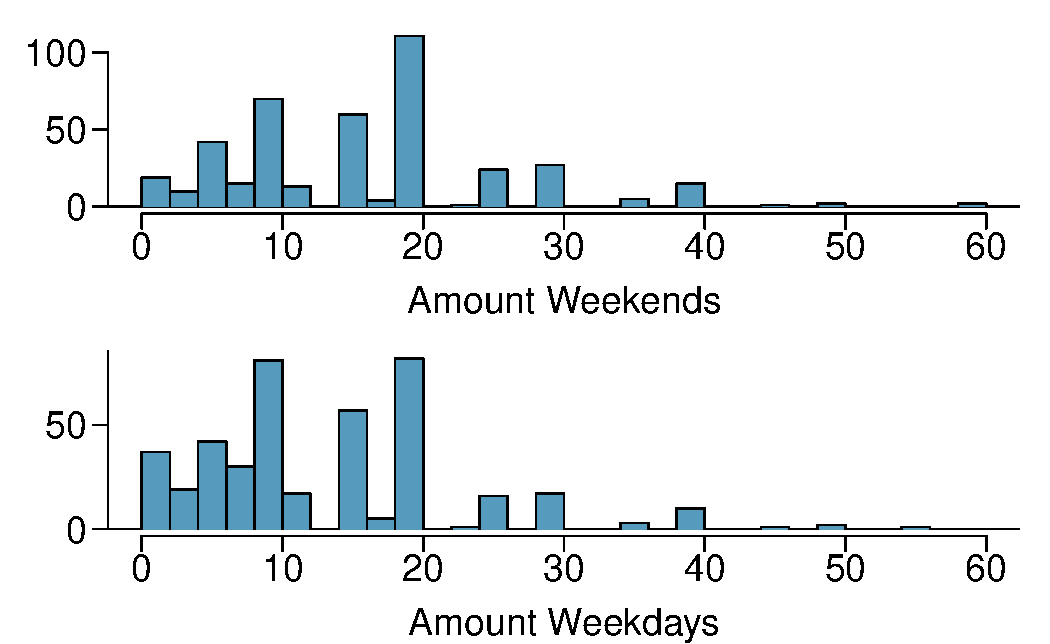
\includegraphics[width = 0.7\textwidth]{ch_summarizing_data/figures/eoce/smoking/smoking_amountHist}
\end{center}
}{}


% 8

\eoce{\qt{Stats scores, Part I\label{stats_final_scores}} Below are the final exam scores of twenty introductory statistics students.
\begin{center}
79, 83, 57, 82, 94, 83, 72, 74, 73, 71, 66, 89, 78, 81, 78, 81, 88, 69, 77, 79
\end{center}
Draw a histogram of these data and describe the distribution.
}{}


% 9

\eoce{\qt{Smoking habits of UK residents, Part II} \label{UKSmoking_amounts_data} A random sample of 5 smokers from the data set discussed in Exercise~\ref{UKSmoking_amounts} is provided below.
{\footnotesize
\begin{center}
\begin{tabular}{ccccccc}
  \hline
gender & age & maritalStatus & grossIncome & smoke & amtWeekends & amtWeekdays \\ 
  \hline
Female &  51 & Married & $\pounds$2,600 to $\pounds$5,200 & Yes &  20 cig/day &  20 cig/day\\ 
  Male &  24 & Single & $\pounds$10,400 to $\pounds$15,600 & Yes &  20 cig/day&  15 cig/day\\ 
  Female &  33 & Married & $\pounds$10,400 to $\pounds$15,600 & Yes &  20 cig/day&  10 cig/day\\ 
  Female &  17 & Single & $\pounds$5,200 to $\pounds$10,400 & Yes &  20 cig/day&  15 cig/day\\ 
  Female &  76 & Widowed & $\pounds$5,200 to $\pounds$10,400 & Yes &  20 cig/day&  20 cig/day\\ 
   \hline
\end{tabular}
\end{center}
}
\begin{parts}
\item Find the mean amount of cigarettes smoked on weekdays and weekends by these 5 respondents.
\item Find the standard deviation of the amount of cigarettes smoked on weekdays and on weekends by these 5 respondents. Is the variability higher on weekends or on weekdays?
\end{parts}
}{}

% 10

\eoce{\qt{Factory defective rate} A factory quality control manager decides to investigate the percentage of defective items produced each day. Within a given work week (Monday through Friday) the percentage of defective items produced was 2\%, 1.4\%, 4\%, 3\%, 2.2\%.
\begin{parts}
\item Calculate the mean for these data.
\item Calculate the standard deviation for these data, showing each step in detail.
\end{parts}
}{}


% 11

\eoce{\qt{Days off at a mining plant\label{days_off_mining}} Workers at a particular mining 
site receive an average of 35 days paid vacation, which is lower than the national 
average. The manager of this plant is under pressure from a local union to increase the 
amount of paid time off. However, he does not want to give more days off to the workers 
because that would be costly. Instead he decides he should fire 10 employees in such a 
way as to raise the average number of days off that are reported by his employees. In 
order to achieve this goal, should he fire employees who have the most number of days 
off, least number of days off, or those who have about the average number of days off?
}{}

\D{\newpage}

% 12

\eoce{\qt{Medians and IQRs} For each part, compare distributions (1) and (2) based on their medians and IQRs. You do not need to calculate these statistics; simply state how the medians and IQRs compare. Make sure to explain your reasoning. 
\begin{multicols}{2}
\begin{parts}
\item (1) 3, 5, 6, 7, 9 \\
(2) 3, 5, 6, 7, 20
\item (1) 3, 5, 6, 7, 9 \\
(2) 3, 5, 7, 8, 9
\item (1) 1, 2, 3, 4, 5 \\
(2) 6, 7, 8, 9, 10
\item (1) 0, 10, 50, 60, 100 \\
(2) 0, 100, 500, 600, 1000
\end{parts}
\end{multicols}
}{}

% 13

\eoce{\qt{Means and SDs} For each part, compare distributions (1) and (2) based on their means and standard deviations. You do not need to calculate these statistics; simply state how the means and the standard deviations compare. Make sure to explain your reasoning. \textit{Hint:} It may be useful to sketch dot plots of the distributions.
\begin{multicols}{2}
\begin{parts}
\item (1) 3, 5, 5, 5, 8, 11, 11, 11, 13 \\
(2) 3, 5, 5, 5, 8, 11, 11, 11, 20 \\
\item (1) -20, 0, 0, 0, 15, 25, 30, 30 \\
(2) -40, 0, 0, 0, 15, 25, 30, 30
\item (1) 0, 2, 4, 6, 8, 10 \\
(2) 20, 22, 24, 26, 28, 30
\item (1) 100, 200, 300, 400, 500 \\
(2) 0, 50, 300, 550, 600
\end{parts}
\end{multicols}
}{}

% 14

\eoce{\qt{Mix-and-match} Describe the distribution in the histograms below and match them to the box plots. \\
\begin{center}
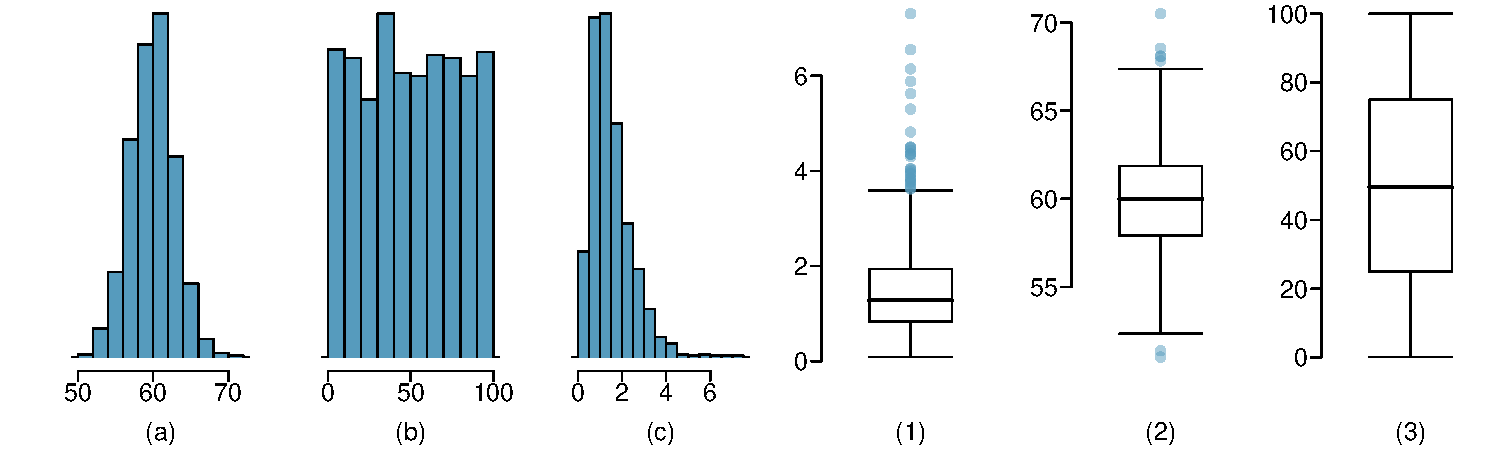
\includegraphics[width=\textwidth]{ch_summarizing_data/figures/eoce/hist_box_match/hist_box_match.pdf}
\end{center}
}{}

% 15

\eoce{\qt{Air quality\label{air_quality_durham}} Daily air quality is measured by the air 
quality index (AQI) reported by the Environmental Protection Agency. This index reports 
the pollution level and what associated health effects might be a concern. The index is 
calculated for five major air pollutants regulated by the Clean Air Act and takes values 
from 0 to 300, where a higher value indicates lower air quality. AQI was reported for a 
sample of 91 days in 2011 in Durham, NC. The relative frequency histogram below shows 
the distribution of the AQI values on these days. \footfullcite{data:durhamAQI:2011} \\
\begin{minipage}[c]{0.55\textwidth}
\begin{parts}
\item Estimate the median AQI value of this sample.
\item Would you expect the mean AQI value of this sample to be higher or lower than the 
median? Explain your reasoning.
\item Estimate Q1, Q3, and IQR for the distribution.
\item Would any of the days in this sample be considered to have an unusually low or 
high AQI? Explain your reasoning.
\end{parts}
\end{minipage}
\begin{minipage}[c]{0.45\textwidth}
\begin{center}
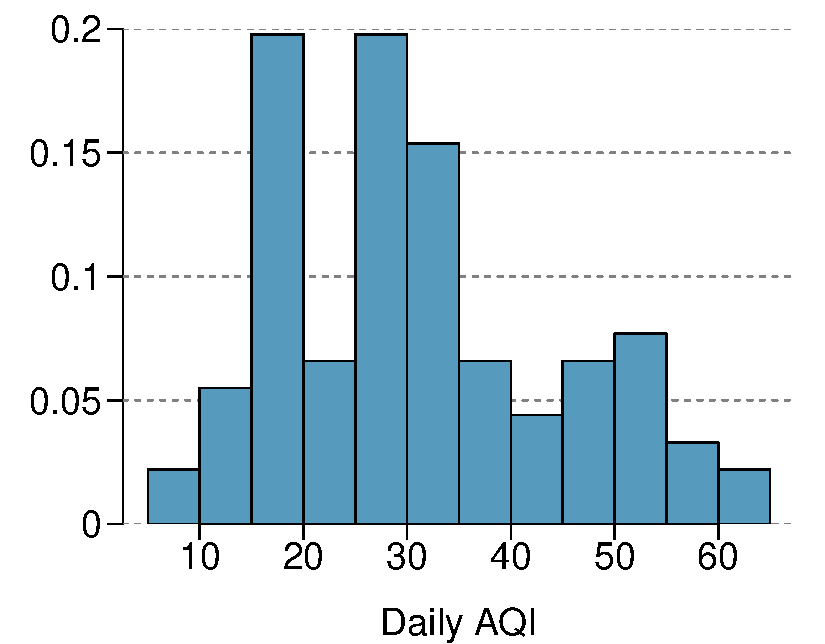
\includegraphics[width = \textwidth]{ch_summarizing_data/figures/eoce/air_quality_durham/air_quality_durham_rel_freq_hist.pdf} 
\end{center}
\end{minipage}
}{}

\D{\newpage}

% 16

\eoce{\qt{Median vs. mean\label{estimate_mean_median_simple}} Estimate the median for the 
400 observations shown in the histogram, and note whether you expect the mean 
to be higher or lower than the median.
\begin{center}
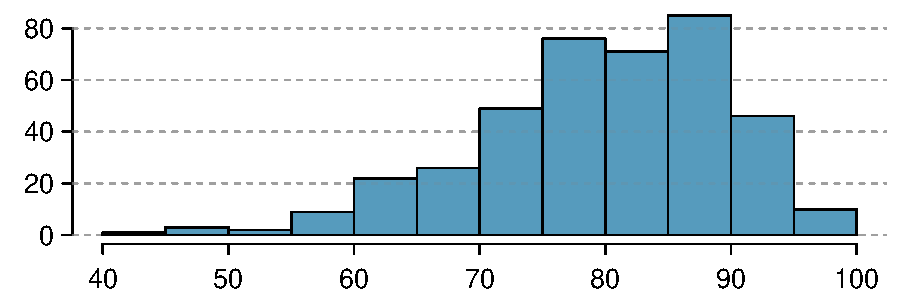
\includegraphics[width = 0.6\textwidth]{ch_summarizing_data/figures/eoce/estimate_mean_median_simple/estimate_mean_median_simple.pdf} 
\end{center}
}{}

% 17

\eoce{\qt{Histograms vs. box plots\label{hist_vs_box}} Compare the two plots below. What 
characteristics of the distribution are apparent in the histogram and not in the box 
plot? What characteristics are apparent in the box plot but not in the histogram?
\begin{center}
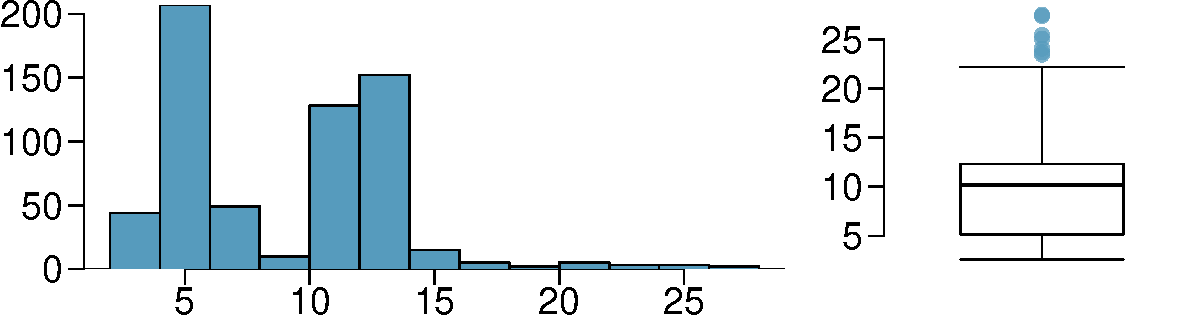
\includegraphics[width = 0.6\textwidth]{ch_summarizing_data/figures/eoce/hist_vs_box/hist_vs_box.pdf}
\end{center}
}{}

% 18

\eoce{\qt{Facebook friends\label{dist_shape_fb_friends}} Facebook data indicate that 
50\% of Facebook users have 100 or more friends, and that the average friend 
count of users is 190. What do these findings suggest about the shape of the 
distribution of number of friends of Facebook users? \footfullcite{Backstrom:2011}
}{}

% 19

\eoce{\qt{Distributions and appropriate statistics, Part I\label{dist_shape_pets_dist_height}} 
For each of the following, state whether you expect the distribution to be 
symmetric, right skewed, or left skewed. Also specify whether the mean or 
median would best represent a typical observation in the data, and whether 
the variability of observations would be best represented using the 
standard deviation or IQR. Explain your reasoning.
\begin{parts}
\item Number of pets per household. 
\item Distance to work, i.e. number of miles between work and home.
\item Heights of adult males.
\end{parts}
}{}

% 20

\eoce{\qt{Distributions and appropriate statistics, Part II\label{dist_shape_housing_alcohol_salary}} 
For each of the following, state whether you expect the distribution to be symmetric, 
right skewed, or left skewed. Also specify whether the mean or median would best 
represent a typical observation in the data, and whether the variability of observations 
would be best represented using the standard deviation or IQR. Explain your reasoning.
\begin{parts}
\item Housing prices in a country where 25\% of the houses cost below \$350,000, 
50\% of the houses cost below \$450,000, 75\% of the houses cost below \$1,000,000 
and there are a meaningful number of houses that cost more than \$6,000,000.
\item Housing prices in a country where 25\% of the houses cost below \$300,000, 
50\% of the houses cost below \$600,000, 75\% of the houses cost below \$900,000 
and very few houses that cost more than \$1,200,000.
\item Number of alcoholic drinks consumed by college students in a given week. 
Assume that most of these students don't drink since they are under 21 years old, 
and only a few drink excessively.
\item Annual salaries of the employees at a Fortune 500 company where only a few 
high level executives earn much higher salaries than all the other employees.
\end{parts}
}{}

\D{\newpage}

% 21

\eoce{\qt{Income at the coffee shop\label{income_coffee_shop}} The first histogram 
below shows the distribution of the yearly incomes of 40 patrons at a college 
coffee shop. Suppose two new people walk into the coffee shop: one making 
\$225,000 and the other \$250,000. The second histogram shows the new income 
distribution. Summary statistics are also provided. \\
\begin{minipage}[c]{0.57\textwidth}
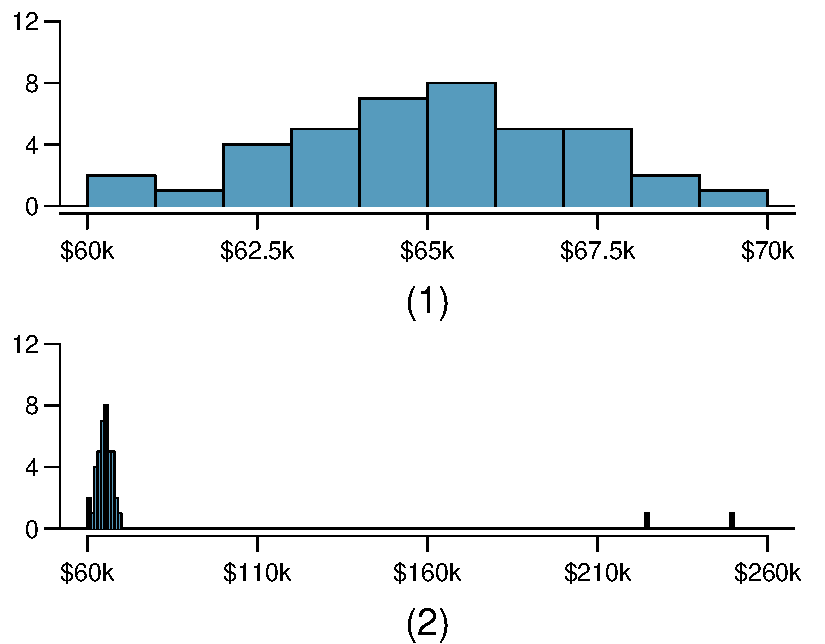
\includegraphics[width=\textwidth]{ch_summarizing_data/figures/eoce/income_coffee_shop/income_coffee_shop.pdf}
\end{minipage}
\begin{minipage}[c]{0.4\textwidth}
\begin{center}
\begin{tabular}{rrr}
\hline
        & (1)       & (2) \\ 
\hline
n       & 40        & 42 \\ 
Min.    & 60,680    & 60,680 \\ 
1st Qu. & 63,620    & 63,710 \\ 
Median  & 65,240    & 65,350 \\ 
Mean    & 65,090    & 73,300 \\ 
3rd Qu. & 66,160    & 66,540 \\ 
Max.    & 69,890    & 250,000 \\ 
SD      & 2,122     & 37,321 \\ 
\hline
\end{tabular}
\end{center}
\end{minipage}
\begin{parts}
\item Would the mean or the median best represent what we might think of as a 
typical income for the 42 patrons at this coffee shop? What does this say about 
the robustness of the two measures?
\item Would the standard deviation or the IQR best represent the amount of 
variability in the incomes of the 42 patrons at this coffee shop? What does 
this say about the robustness of the two measures?
\end{parts}
}{}

% 22

\eoce{\qt{Midrange\label{midrange}} The \textit{midrange} of a distribution is defined as 
the average of the maximum and the minimum of that distribution. Is this statistic 
robust to outliers and extreme skew? Explain your reasoning
}{}

% 23

\eoce{\qt{Commute times\label{county_commute_times}} The US census collects data on 
time it takes Americans to commute to work, among many other variables. The 
histogram below shows the distribution of average commute times in 3,142 US 
counties in 2017. 
\begin{center}
\href{\oiRedirectUrl{tableau-histogramschoose}}{
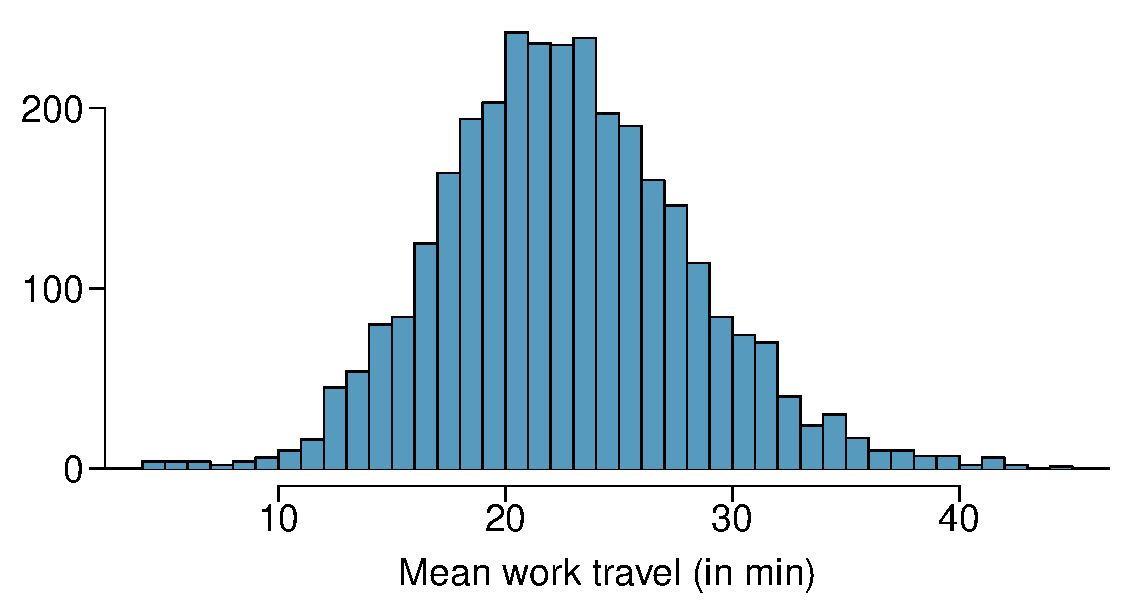
\includegraphics[width=0.45\textwidth]{ch_summarizing_data/figures/eoce/county_commute_times/county_commute_times_hist.pdf}
}\tableauhref{tableau-histogramschoose}
\href{\oiRedirectUrl{tableau-intensitymapsall}}{
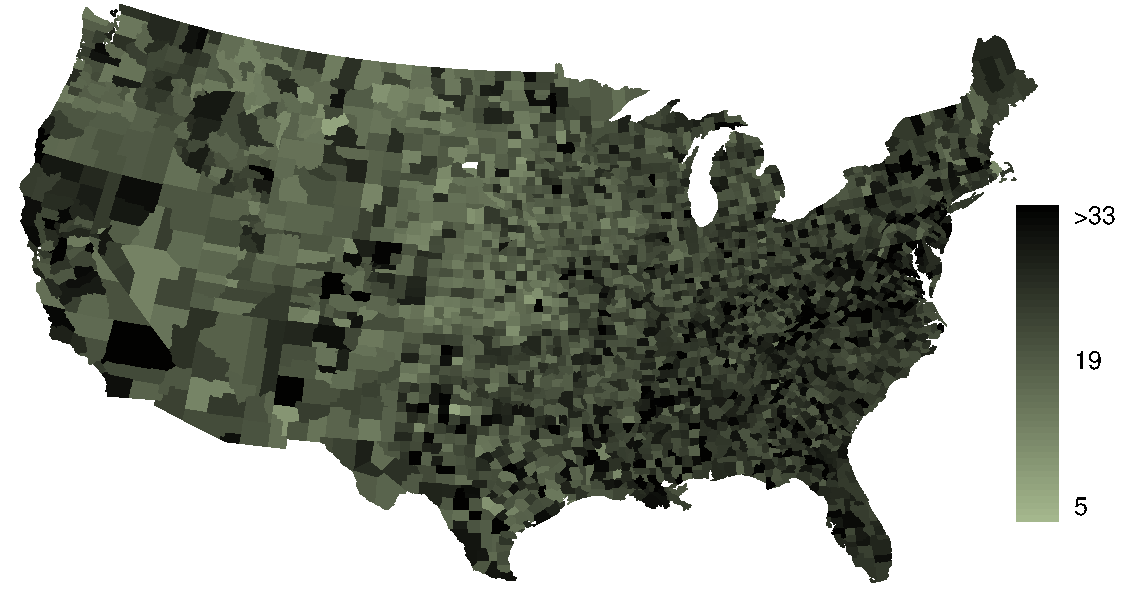
\includegraphics[width=0.45\textwidth]{ch_summarizing_data/figures/eoce/county_commute_times/county_commute_times_map.pdf}
}\tableauhref{tableau-intensitymapsall}
\end{center}
\begin{parts}
\item Describe the distribution of average commute times for counties in the US.
\item Describe the spatial distribution of commuting times using the map provided.
\end{parts} 
}{}


% 24

\eoce{\qt{Hispanic/Latinx population\label{county_hispanic_pop}} The US census collects 
data on race and ethnicity of Americans, among many other variables. The 
histogram below shows the distribution of the percentage of the population 
that is Hispanic/Latinx in 3,142 counties in the US in 2017. \begin{center}
\href{\oiRedirectUrl{tableau-histogramschoose}}{
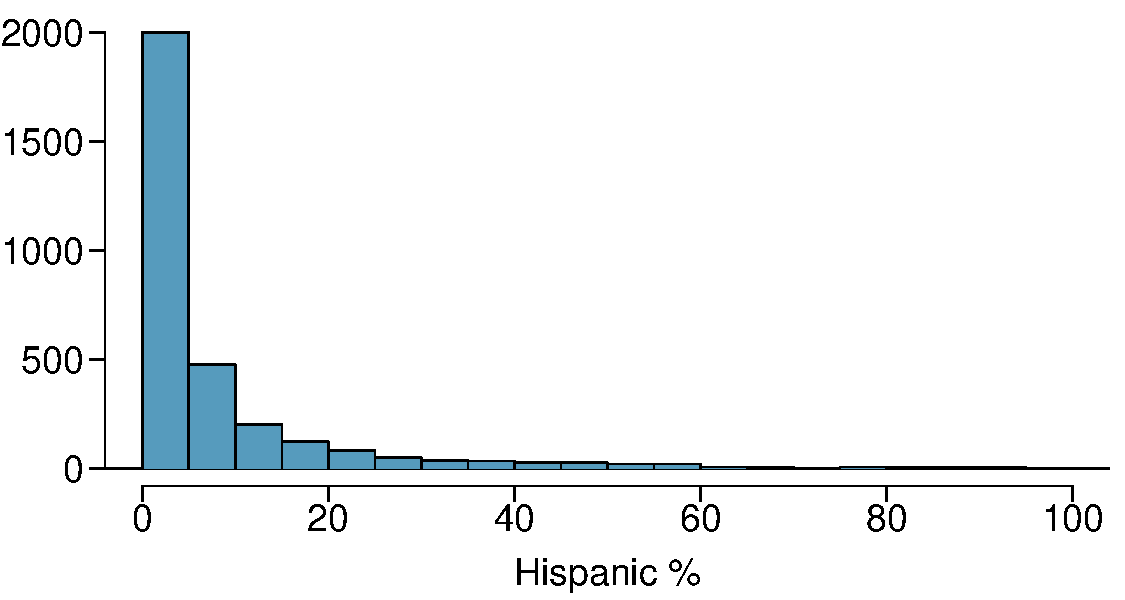
\includegraphics[width=0.45\textwidth]{ch_summarizing_data/figures/eoce/county_hispanic_pop/county_hispanic_pop_hist.pdf}
}\tableauhref{tableau-histogramschoose}
\href{\oiRedirectUrl{tableau-intensitymapsall}}{
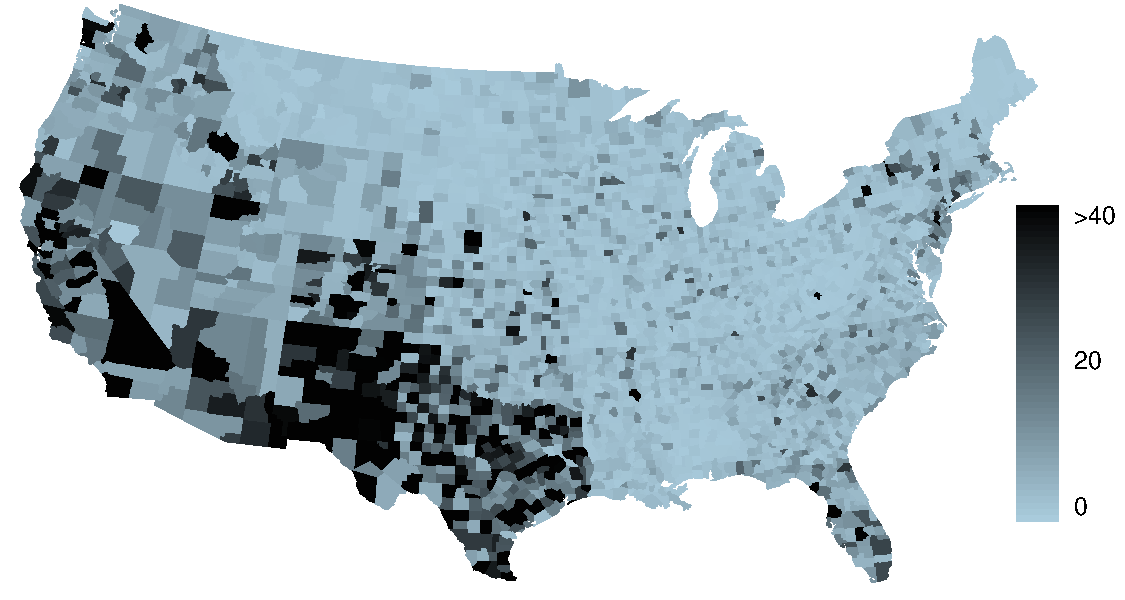
\includegraphics[width=0.45\textwidth]{ch_summarizing_data/figures/eoce/county_hispanic_pop/county_hispanic_pop_map.pdf}
}\tableauhref{tableau-intensitymapsall}
\end{center}
\begin{parts}
\item Describe the distribution of percent of population that is Hispanic/Latinx for counties in the US.
\item What features of the distribution of the Hispanic/Latinx population in US 
counties are apparent in the map but not in the histogram? What features are 
apparent in the histogram but not the map?
%\item Is one visualization more appropriate or helpful than the other? Explain 
%your reasoning.
\end{parts} 
}{}
}


%______________________________________________
\section[Considering categorical data]{Considering categorical data }
\label{categoricalData}
\index{data!email|(}

\sectionintro{

\noindent%
How do we visualize and summarize categorical data?
In this section, we will introduce tables and other basic tools for categorical data that are used throughout this book and will answer the following questions:

\begin{itemize}
\item Based on the \data{loan50} data, is there an assocation between the categorical variables of homeownership and application type (individual, joint)?

\item Using the \data{email50} data, does email type provide any useful value in classifying email as spam or not spam?  

\end{itemize}


% library(openintro); data(email); dim(email)

%%
\subsection*{Learning objectives}
\begin{enumerate}
\setlength{\itemsep}{0mm}
\item Use a one-way table and a bar~chart to summarize a categorical variable.  Use counts (frequency) or proportions (relative frequency).

\item Compare distributions of a categorical variable using a two-way table and a side-by-side bar~chart, segmented bar~chart, or mosaic plot.

\item Calculate marginal and joint frequencies for two-way tables.

\end{enumerate}
}


%%
\subsection{Contingency tables and bar~charts}
% library(openintro); dim(loans_full_schema)

\newcommand{\loanapphomeAA}{3496}
\newcommand{\loanapphomeAB}{3839}
\newcommand{\loanapphomeAC}{1170}
\newcommand{\loanapphomeAD}{8505}
\newcommand{\loanapphomeBA}{362}
\newcommand{\loanapphomeBB}{950}
\newcommand{\loanapphomeBC}{183}
\newcommand{\loanapphomeBD}{1495}
\newcommand{\loanapphomeDA}{3858}
\newcommand{\loanapphomeDAPt}{0.3858} % Overall frequency
\newcommand{\loanapphomeDB}{4789}
\newcommand{\loanapphomeDC}{1353}
\newcommand{\loanapphomeDD}{10000}
\newcommand{\loanapphomeN}{\loanapphomeDD{}}
\index{data!loans|(}

Figure~\ref{loan_home_app_type_totals} summarizes two variables:
\var{app\us{}type}
%\footnote{For those readers already familiar
%  with \emph{joint probabilities}, \resp{joint} in the table
%  refers to a level of the \var{app\us{}type} variable
%  for a joint application.
%  The does not refer to a joint probability!}
and \var{homeownership}.
A table that summarizes data for two categorical variables in
this way is called a \term{contingency table}.
Each value in the table represents the number of times
a particular combination of variable outcomes occurred.
For example, the value \loanapphomeAA{} corresponds to the number of
loans in the data set where the borrower rents their home
and the application type was by an individual.
Row and column totals are also included.
The \term{row totals} \index{contingency table!row totals}
provide the total counts across each row
(e.g. $\loanapphomeAA{} + \loanapphomeAB{} +
  \loanapphomeAC{} = \loanapphomeAD{}$),
and \term{column totals} \index{contingency table!column totals}
are total counts down each column.
We can also create a table that shows only the overall 
percentages or proportions for each combination of categories,
or we can create a table for a single variable,
such as the one shown in Figure~\ref{loan_homeownership_totals}
for the \var{homeownership} variable.

\begin{figure}[ht]
\centering
\begin{tabular}{ll  ccc  rr}
  & & \multicolumn{3}{c}{\bf \var{homeownership}} & \\
  \cline{3-5}
  & & rent & mortgage & own & Total & \hspace{2mm}\  \\ 
  \cline{2-6}
  & individual &
      \loanapphomeAA{} &
      \loanapphomeAB{} &
      \loanapphomeAC{} &
      \loanapphomeAD{} \\
  \raisebox{1.5ex}[0pt]{\var{app\us{}type}} &
  joint &
      \loanapphomeBA{} &
      \loanapphomeBB{} &
	  \loanapphomeBC{} &
	  \loanapphomeBD{} \\
  \cline{2-6}
  & Total &
      \loanapphomeDA{} &
      \loanapphomeDB{} &
      \loanapphomeDC{} &
      \loanapphomeDD{} \\
  \cline{2-6}
\end{tabular}
\caption{A contingency table for
    \var{app\us{}type} and \var{homeownership}.}
\label{loan_home_app_type_totals}
%library(openintro); library(xtable); tab <- table(loans_full_schema[,c("application_type", "homeownership")])[, c("RENT", "MORTGAGE", "OWN")]; xtable(tab); rowSums(tab); colSums(tab); sum(tab)
\end{figure}

\begin{figure}[htb]
\centering
\begin{tabular}{lc}
  \hline
  \var{homeownership} & Count \\
  \hline
  rent & \loanapphomeDA{} \\
  mortgage & \loanapphomeDB{} \\
  own & \loanapphomeDC{} \\
  \hline
  Total & \loanapphomeDD{} \\ 
  \hline
\end{tabular}
\caption{A table summarizing the frequencies of each
    value for the \var{homeownership} variable.}
\label{loan_homeownership_totals}
\end{figure}

A \term{bar~chart} (also called bar~plot or bar~chart) is a common way to display a single
categorical variable.
The left panel of Figure~\ref{loan_homeownership_bar_plot}
shows a bar~chart for the \var{homeownership} variable.
In the right panel, the counts are converted into proportions,
showing the proportion of observations that are in each level
(e.g. $\loanapphomeDA{} / \loanapphomeDD{} = 0.3858$ for
  \resp{rent}).

\begin{figure}[bht]
  \centering
  \Figure{0.82}{loan_homeownership_bar_plot}
  \caption{Two bar~charts of \var{number}.
      The left panel shows the counts, and the right panel
      shows the proportions in each group.}
  \label{loan_homeownership_bar_plot}
\end{figure}


\D{\newpage}

\subsection{Row and column proportions}

Sometimes it is useful to understand the fractional breakdown
of one variable in another,
and we can modify our contingency table to provide such a view.
Figure~\ref{rowPropAppTypeHomeownership}
shows the
\termsub{row proportions}{contingency table!row proportions}
for Figure~\ref{loan_home_app_type_totals},
which are computed as the counts divided by their row totals.
The value \loanapphomeAA{} at the intersection of
\resp{individual} and \resp{rent} is replaced by
$\loanapphomeAA{}/\loanapphomeAD{} = 0.411$,
i.e. \loanapphomeAA{} divided by its row total,
\loanapphomeAD{}.
So what does 0.411 represent?
It corresponds to the proportion of individual
applicants who rent.

\begin{figure}[h]
\centering
\begin{tabular}{l rrr r}
  \hline
  & rent & mortgage & own & Total \\
  \hline
  individual & 
%      $\loanapphomeAA{}/\loanapphomeAD{} = 0.411$ &
%      $\loanapphomeAB{}/\loanapphomeAD{} = 0.451$ &
%      $\loanapphomeAC{}/\loanapphomeAD{} = 0.138$ &
      0.411 &
      0.451 &
      0.138 &
      1.000 \\
  joint &
%      $\loanapphomeBA{}/\loanapphomeBD{} = 0.242$ &
%      $\loanapphomeBB{}/\loanapphomeBD{} = 0.635$ &
%      $\loanapphomeBC{}/\loanapphomeBD{} = 0.122$ &
      0.242 &
      0.635 &
      0.122 &
      1.000 \\
  \hline
  Total &
%      $\loanapphomeDA{}/\loanapphomeDD{} = 0.386$ &
%      $\loanapphomeDB{}/\loanapphomeDD{} = 0.479$ &
%      $\loanapphomeDC{}/\loanapphomeDD{} = 0.135$ &
      0.386 &
      0.479 &
      0.135 &
      1.000 \\
  \hline
\end{tabular}
\caption{A contingency table with row proportions
    for the \var{app\us{}type} and
    \var{homeownership} variables.
    The row total is off by 0.001 for the
    \resp{joint} row due to a rounding error.}
\label{rowPropAppTypeHomeownership}
\end{figure}

A contingency table of the column proportions is computed in a similar way, where each \termsub{column proportion}{contingency table!column proportion} is computed as the count divided by the corresponding column total. Figure~\ref{colPropAppTypeHomeownership} shows such a table, and here the value 0.906 indicates that 90.6\% of renters applied as individuals for the loan. This rate is higher compared to loans from people with mortgages (80.2\%) or who own their home (85.1\%). Because these rates vary between the three levels of \var{homeownership} (\resp{rent}, \resp{mortgage}, \resp{own}), this provides evidence that the \var{app\us{}type} and \var{homeownership} variables are associated.

\begin{figure}[h]
\centering%\small
\begin{tabular}{l rrr r}
  \hline
  & rent & mortgage & own & Total \\
  \hline
  individual &
%      $\loanapphomeAA{}/\loanapphomeDA{} = 0.906$ &
%      $\loanapphomeAB{}/\loanapphomeDB{} = 0.802$ &
%      $\loanapphomeAC{}/\loanapphomeDC{} = 0.865$ &
%      $\loanapphomeAD{}/\loanapphomeDD{} = 0.851$ \\
      0.906 &
      0.802 &
      0.865 &
      0.851 \\
  joint &
%      $\loanapphomeBA{}/\loanapphomeDA{} = 0.094$ &
%      $\loanapphomeBB{}/\loanapphomeDB{} = 0.198$ &
%      $\loanapphomeBC{}/\loanapphomeDC{} = 0.135$ &
%      $\loanapphomeBD{}/\loanapphomeDD{} = 0.150$ \\
      0.094 &
      0.198 &
      0.135 &
      0.150 \\
  \hline
  Total & 1.000 & 1.000 & 1.000 & 1.000 \\
  \hline
\end{tabular}
\caption{A contingency table with column proportions for the
    \var{app\us{}type} and \var{homeownership}
    variables.
    The total for the last column is off by 0.001 due
    to a rounding error.}
\label{colPropAppTypeHomeownership}
\end{figure}

We could also have checked for an association between \var{app\us{}type} and \var{homeownership} in Figure~\ref{rowPropAppTypeHomeownership} using row proportions. When comparing these row proportions, we would look down columns to see if the fraction of loans where the borrower rents, has a mortgage, or owns varied across the \resp{individual} to \resp{joint} application types.

\begin{exercisewrap}
\begin{nexercise}
(a)~What does 0.451 represent in
Figure~\ref{rowPropAppTypeHomeownership}?

(b)~What does 0.802 represent in
Figure~\ref{colPropAppTypeHomeownership}?\footnotemark{}
\end{nexercise}
\end{exercisewrap}
\footnotetext{(a)~0.451 represents the proportion of individual
  applicants who have a mortgage.
  (b)~0.802 represents the fraction
  of applicants with mortgages who applied as individuals.}

\begin{exercisewrap}
\begin{nexercise}
(a)~What does 0.122 at the intersection of \resp{joint} and
\resp{own} represent in
Figure~\ref{rowPropAppTypeHomeownership}?

(b)~What does 0.135 represent in the
Figure~\ref{colPropAppTypeHomeownership}?\footnotemark{}
\end{nexercise}
\end{exercisewrap}
\footnotetext{(a)~0.122 represents the fraction of joint borrowers
  who own their home.
  (b)~0.135 represents the home-owning borrowers
  who had a joint application for the loan.}


\begin{examplewrap}
\begin{nexample}{
    Data scientists use statistics to filter spam from incoming
    email messages.
    By noting specific characteristics of an email,
    a data scientist may be able to classify some emails as spam
    or not spam with high accuracy.
    One such characteristic is whether the email
    contains no numbers, small numbers, or big numbers.
    Another characteristic is the email format, which
    indicates whether or not an email has any HTML content,
    such as bolded text.
    We'll focus on email format and spam status using the
    \data{email} data set, and these variables are summarized
    in a contingency table in
    Figure~\ref{emailSpamHTMLTableTotals}.
    Which would be more helpful to someone hoping to classify
    email as spam or regular email for this table:
    row or column proportions?}
  \label{weighingRowColumnProportions}
  A data scientist would be interested in how the proportion
  of spam changes within each email format.
  This corresponds to column proportions:
  the proportion of spam in plain text emails
  and the proportion of spam in HTML emails.

  If we generate the column proportions, we can see
  that a higher fraction of plain text emails are
  spam ($209/1195 = 17.5\%$)
  than compared to HTML emails ($158/2726 = 5.8\%$).
  This information on its own is insufficient to classify
  an email as spam or not spam, as over 80\% of plain text
  emails are not spam.
  Yet, when we carefully combine this information with many
  other characteristics,
  we stand a reasonable chance of being able to classify
  some emails as spam or not spam with confidence.
\end{nexample}
\end{examplewrap}

\begin{figure}[ht]
\centering
\begin{tabular}{l cc r}
  \hline
  & text & HTML & Total \\ 
  \hline
  spam & 209 & 158 & 367 \\ 
  not spam & 986 & 2568 & 3554 \\ 
  \hline
  Total & 1195 & 2726 & 3921 \\
  \hline
\end{tabular}
\caption{A contingency table for \var{spam} and \var{format}.}
\label{emailSpamHTMLTableTotals}
%library(openintro); library(xtable); data(email); tab <- table(email[,c("spam", "format")])[2:1,]; tab; colSums(tab); rowSums(tab)
\end{figure}

Example~\ref{weighingRowColumnProportions} points out
that row and column proportions are not equivalent.
Before settling on one form for a table,
it is important to consider each to ensure that the
most useful table is constructed.
However, sometimes it simply isn't clear which, if either,
is more useful.

\newpage
\begin{examplewrap}
\begin{nexample}{Look back to
    Tables~\ref{rowPropAppTypeHomeownership}
    and~\ref{colPropAppTypeHomeownership}.
    Are there any obvious scenarios where one might be more
    useful than the other?}
  None that we thought were obvious!
  What is distinct about \var{app\us{}type}
  and \var{homeownership} vs the email example is that
  these two variables don't have a clear explanatory-response
  variable relationship that we might hypothesize
  (see Section~\ref{explanatoryAndResponse} for these terms).
  Usually it is most useful to ``condition'' on the
  explanatory variable.
  For instance, in the email example, the email format
  was seen as a possible explanatory variable of whether
  the message was spam, so we would find it more interesting
  to compute the relative frequencies (proportions)
  for each email format.
\end{nexample}
\end{examplewrap}

%\Comment{Any risk with the above example that students
%  would think they need not know how to describe (what
%  are effectively) conditional probabilities based
%  on row or column proportions?
%  If so, we could add in an exercise that calls this
%  out and requires them to create such a description.}



\subsection{Using a bar~chart with two variables}
\label{bar_plots_subsection}

Contingency tables using row or column proportions
are especially useful for examining how two categorical
variables are related.
Stacked bar~charts provide a way to visualize
the information in these tables.

A \termsub{segmented bar~chart}{bar chart!segmented bar chart}, or stacked bar~chart,
\index{bar chart!stacked bar chart}
is a graphical display of contingency table information.
For example, a~segmented bar~chart representing
Figure~\ref{colPropAppTypeHomeownership}
is shown in Figure~\ref{loan_app_type_home_seg_bar},
where we have first created a bar~chart using the
\var{homeownership} variable and then divided each group
by the levels of \mbox{\var{app\us{}type}}.

One related visualization to the segmented bar~chart is the
\termsub{side-by-side bar~chart}{bar chart!side-by-side},
where an example is shown in
Figure~\ref{loan_app_type_home_sbs_bar}.

For the last type of bar~chart we introduce,
the column proportions for the
\var{app\us{}type} and \var{homeownership} contingency table
have been translated into a standardized segmented bar~chart
in Figure~\ref{loan_app_type_home_seg_bar_standardized}.
This type of visualization is helpful in understanding
the fraction of individual or joint loan applications
for borrowers in each level of \var{homeownership}.
Additionally, since the proportions of \resp{joint}
and \resp{individual} vary across the groups,
we can conclude that the two variables are associated.

\newcommand{\loanapptypehomesegbarplotwidth}{0.46\textwidth}
\begin{figure}[h]
  \centering
\oiRedirect{tableau-bargraphs2V}{
  \subfigure[]{
    \Figuress{\loanapptypehomesegbarplotwidth}
        {loan_app_type_home_seg_bar}
        {loan_app_type_home_seg_bar}
    \label{loan_app_type_home_seg_bar}
  }
  \subfigure[]{
    \Figuress{\loanapptypehomesegbarplotwidth}
        {loan_app_type_home_seg_bar}
        {loan_app_type_home_sbs_bar}
    \label{loan_app_type_home_sbs_bar}
  }
  \subfigure[]{
    \Figuress{\loanapptypehomesegbarplotwidth}
        {loan_app_type_home_seg_bar}
        {loan_app_type_home_seg_bar_standardized}
    \label{loan_app_type_home_seg_bar_standardized}
  }
  \subfigure[]{
    \Figuress{\loanapptypehomesegbarplotwidth}
        {loan_app_type_home_seg_bar}
        {loan_app_type_home_sbs_bar_standardized}
    \label{loan_app_type_home_sbs_bar_standardized}
  }}
%  \subtable{
%    \footnotesize
%    \begin{tabular}{l  ccc  r}
%      \multicolumn{5}{l}{Contingency table summarizing}\\
%      \multicolumn{5}{l}{application type and homeownership:} \\
%      \\
%      & \multicolumn{3}{c}{\bf \var{homeownership}} & \\
%      \cline{2-4}
%      \var{app\us{}type} &
%          rent & mortgage & own & Total \\ 
%      \hline
%      individual &
%          \loanapphomeAA{} &
%          \loanapphomeAB{} &
%          \loanapphomeAC{} &
%          \loanapphomeAD{} \\
%      joint &
%          \loanapphomeBA{} &
%          \loanapphomeBB{} &
%    	  \loanapphomeBC{} &
%    	  \loanapphomeBD{} \\
%      \hline
%      Total &
%          \loanapphomeDA{} &
%          \loanapphomeDB{} &
%          \loanapphomeDC{} &
%          \loanapphomeDD{} \\
%      \hline
%      \ \\
%      \ \\
%      \multicolumn{5}{l}{Version of the table}\\
%      \multicolumn{5}{l}{with column proportions:} \\
%      \\
%      & \multicolumn{3}{c}{\bf \var{homeownership}} & \\
%      \cline{2-4}
%      \var{app\us{}type} &
%          rent & mortgage & own & Total \\ 
%      \hline
%      individual &
%          0.906 &
%          0.802 &
%          0.865 &
%          0.851 \\
%      joint &
%          0.094 &
%          0.198 &
%          0.135 &
%          0.150 \\
%      \hline
%      Total & 1.000 & 1.000 & 1.000 & 1.000 \\
%      \hline
%      \ \\
%    \end{tabular}
%    \label{loan_app_type_home_copied_table}
%  }
  \caption{\subref{loan_app_type_home_seg_bar} segmented
      bar~chart for \var{homeownership},
      where the counts have been further broken down
      by \var{app\us{}type}.
      \subref{loan_app_type_home_sbs_bar}~Side-by-side
      bar~chart for \var{homeownership}
      and \var{app\us{}type}.
      \subref{loan_app_type_home_seg_bar_standardized}~Standardized
      version of the segmented bar~chart.
      \subref{loan_app_type_home_sbs_bar_standardized}~Standardized
      side-by-side bar~chart.
      See these bar charts on Tableau Public~\tableauhref{tableau-bargraphs2V}.}
  \label{loan_app_type_home_seg_bar_plot}
\end{figure}

\begin{examplewrap}
\begin{nexample}{Examine the four bar~charts in
    Figure~\ref{loan_app_type_home_seg_bar_plot}.
    When is the segmented, side-by-side, standardized
    segmented bar~chart, or standardized side-by-side the most useful?}
  The segmented bar~chart is most useful when it's reasonable
  to assign one variable as the explanatory variable and
  the other variable as the response, since we are effectively
  grouping by one variable first and then breaking it down by
  the others.

  Side-by-side bar~charts are more agnostic in their display
  about which variable, if any, represents the explanatory
  and which the response variable.
  It is also easy to discern the number of cases
  in of the six different group combinations.
  However, one downside
  is that it tends to require more horizontal space;
  the narrowness of Figure~\ref{loan_app_type_home_sbs_bar}
  makes the plot feel a bit cramped.
  Additionally, when two groups are of very different sizes,
  as we see in the \resp{own} group relative to either of the
  other two groups,
  it is difficult to discern if there is an association
  between the variables.

  The standardized segmented bar~chart is helpful if the primary
  variable in the segmented bar~chart is relatively imbalanced,
  e.g. the \resp{own} category has only a third of the
  observations in the \resp{mortgage} category,
  making the simple segmented bar~chart less useful for
  checking for an association.
  The major downside of the standardized version
  is that we lose all sense of how many cases each of the
  bars represents.
\end{nexample}
\end{examplewrap}

\newpage
\subsection{Mosaic plots}
\label{mosaic_plots_subsection}

A \term{mosaic plot} is a visualization technique
suitable for contingency tables that resembles
a standardized segmented bar~chart with the benefit
that we still see the relative group sizes of the
primary variable as well.

To get started in creating our first mosaic plot,
we'll break a square into columns for each category
of the \var{homeownership} variable,
with the result shown in Figure~\ref{loan_home_mosaic}.
Each column represents a level of \var{homeownership},
and the column widths correspond to the proportion of
loans in each of those categories.
For~instance, there are fewer loans where the borrower
is an owner than where the borrower has a mortgage.
In general, mosaic plots use box \emph{areas}
to represent the number of cases in each category.

\begin{figure}[h]
  \centering
  \subfigure[]{
    \Figures{0.36}
        {loan_app_type_home_mosaic_plot}
        {loan_home_mosaic}
    \label{loan_home_mosaic}
  }
  \subfigure[]{
    \Figures{0.44}
        {loan_app_type_home_mosaic_plot}
        {loan_app_type_home_mosaic}
    \label{loan_app_type_home_mosaic}
  }
  \caption{\subref{loan_home_mosaic}~The one-variable mosaic
      plot for \var{homeownership}.
      \subref{loan_app_type_home_mosaic}~Two-variable mosaic
      plot for both \var{homeownership}
      and \var{app\us{}type}.}
  \label{loan_app_type_home_mosaic_plot}
\end{figure}

To create a completed mosaic plot, the single-variable
mosaic plot is further divided into pieces in
Figure~\ref{loan_app_type_home_mosaic} using the
\var{app\us{}type} variable.
Each column is split proportional to the
number of loans from individual and joint
borrowers.
For example, the second column represents loans
where the borrower has a mortgage,
and it was divided into individual loans (upper)
and joint loans (lower).
As another example, the bottom segment of the third column
represents loans where the borrower owns their home
and applied jointly, while the upper segment
of this column represents
borrowers who are homeowners and filed individually.
We can again use this plot to see that
the \var{homeownership} and \var{app\us{}type}
variables are associated, since some columns are divided
in different vertical locations than others,
which was the same technique used for checking an
association in the standardized segmented bar~chart.

\newpage

In Figure~\ref{loan_app_type_home_mosaic_rev},
we chose to first split by the homeowner status
of the borrower.
However, we could have instead first split by
the application type, as in
Figure~\ref{loan_app_type_home_mosaic_rev}.
Like with the bar~charts, it's common to use
the explanatory variable to represent the
first split in a mosaic plot,
and then for the response to break
up each level of the explanatory variable,
if these labels are reasonable to attach to
the variables under consideration.

\begin{figure}[h]
  \centering
  \Figures{0.5}
      {loan_app_type_home_mosaic_plot}
      {loan_app_type_home_mosaic_rev}
  \caption{Mosaic plot where loans are grouped by
      the \var{homeownership} variable after they've
      been divided into the \resp{individual} and
      \resp{joint} application types.}
  \label{loan_app_type_home_mosaic_rev}
\end{figure}

%In a similar way, a mosaic plot representing row proportions of Figure~\ref{loan_home_app_type_totals} could be constructed, as shown in Figure~\ref{loan_app_type_home_mosaic_rev}. However, because it is more insightful for this application to consider the fraction of spam in each category of the \var{number} variable, we prefer Figure~\ref{loan_app_type_home_mosaic}.

\newpage 
%
\subsection{The only pie chart you will see in this book}

A \term{pie chart} is shown in
Figure~\ref{loan_homeownership_pie_chart} alongside
a bar~chart representing the same information.
Pie charts can be useful for giving a high-level overview
to show how a set of cases break down.
However, it is also difficult to decipher details
in a pie chart.
For example, it takes a couple seconds longer to recognize
that there are more loans where the borrower has
a mortgage than rent when looking at the pie chart,
while this detail is very obvious in the bar~chart.
While pie charts can be useful, we prefer bar~charts
for their ease in comparing groups.
%One benefit of pie charts is that they to make it easier
%to see when a series of groups make up at least 50\%,
%e.g. \Comment{would need to show a pie chart with
%  a large number of categories for this point to make sense}.

\begin{figure}[h]
  \centering
\oiRedirect{tableau-bargraphs1V}{
  \Figure{}{loan_homeownership_pie_chart}}
  \caption{A pie chart and bar~chart of \var{homeownership}.  Compare multiple ways of summarizing a single categorical variable on Tableau Public~\tableauhref{tableau-bargraphs1V}.}
  \label{loan_homeownership_pie_chart}
\end{figure}

\index{data!loans|)}



%%
\subsection*{Section summary}
\begin{itemize}
\item \termsub{Categorical variables}{categorical variable}, unlike numerical variables, are simply summarized by \term{counts} (how many) and \termsub{proportions}{proportion}.  These are referred to as frequency and relative frequency, respectively.

\item When summarizing one categorical variable, a \term{one-way frequency table} is useful.  For summarizing two categorical variables and their relationship, use a \term{two-way frequency table} (also known as a contingency table).

\item To graphically summarize a single categorical variable, use a \term{bar~chart}.  To summarize and compare two categorical variables, use a \term{side-by-side bar~chart}, a \term{segmented bar~chart}, or a \term{mosaic plot}.

\item \termsub{Pie charts}{pie chart} are another option for summarizing categorical data, but they are more difficult to read and bar~charts are generally a better option.  
\end{itemize}




%%%%%%%%%%%Section Exercises
{\exercisesheader{}

% 37 - antibiotic_use_children

\eoce{\qt{Antibiotic use in children\label{antibiotic_use_children}} The bar plot 
and the pie chart below show the distribution of pre-existing medical 
conditions of children involved in a study on the optimal duration of 
antibiotic use in treatment of tracheitis, which is an upper respiratory 
infection.
\begin{center}
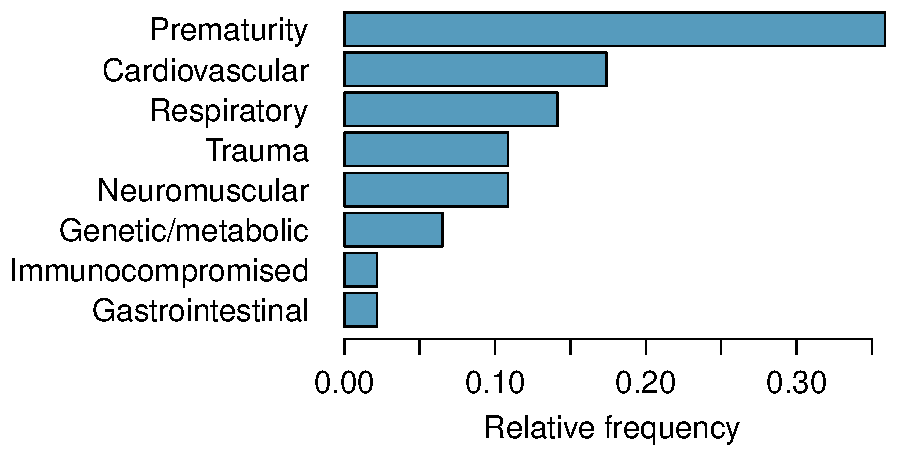
\includegraphics[width = 0.45\textwidth]{ch_summarizing_data/figures/eoce/antibiotic_use_children/antibiotic_use_children_bar}
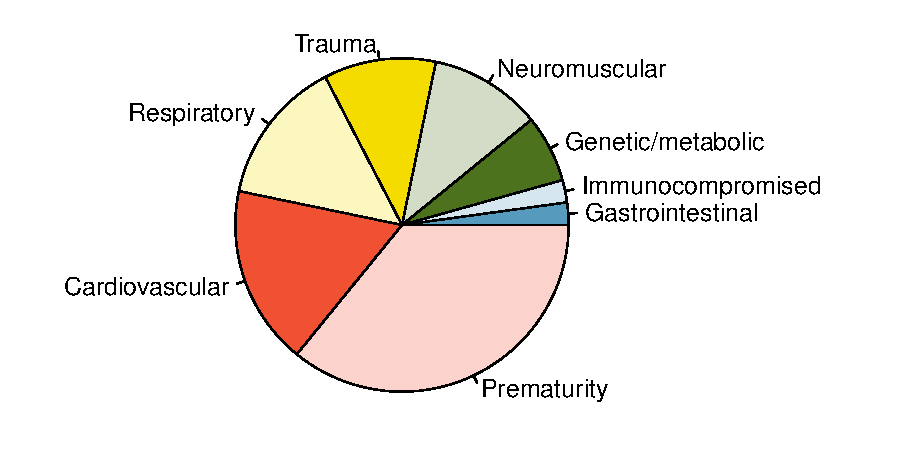
\includegraphics[width = 0.45\textwidth]{ch_summarizing_data/figures/eoce/antibiotic_use_children/antibiotic_use_children_pie}
\end{center}
\begin{parts}
\item What features are apparent in the bar plot but not in the pie chart?
\item What features are apparent in the pie chart but not in the bar plot?
\item Which graph would you prefer to use for displaying these categorical data?
\end{parts}
}{}

% 38 - immigration_contingency_table

\eoce{\qt{Views on immigration\label{immigration}} 910 randomly sampled registered 
voters from Tampa, FL were asked if they thought workers who have illegally 
entered the US should be (i) allowed to keep their jobs and apply for 
US citizenship, (ii) allowed to keep their jobs as temporary guest workers 
but not allowed to apply for US citizenship, or (iii) lose their jobs and 
have to leave the country. The results of the survey by political ideology 
are shown below.\footfullcite{survey:immigFL:2012}
\begin{center}
\begin{tabular}{l l c c c c}
                        &                           & \multicolumn{3}{c}{\textit{Political ideology}} \\
\cline{3-5}
                        &                           & Conservative  & Moderate  & Liberal   & Total \\
\cline{2-6}
                        & (i) Apply for citizenship & 57            & 120       & 101       & 278 \\
                        & (ii) Guest worker         & 121           & 113       & 28        & 262 \\
\raisebox{1.5ex}[0pt]{\emph{Response}} & (iii) Leave the country    & 179       & 126       & 45        & 350 \\ 
                        & (iv) Not sure             & 15            & 4         & 1         & 20\\
\cline{2-6}
                        & Total                     & 372           & 363       & 175       & 910
\end{tabular}
\end{center}
\begin{parts}
\item What percent of these Tampa, FL voters identify themselves as conservatives?
\item What percent of these Tampa, FL voters are in favor of the citizenship option?
\item What percent of these Tampa, FL voters identify themselves as conservatives 
and are in favor of the citizenship option?
\item What percent of these Tampa, FL voters who identify themselves as 
conservatives are also in favor of the citizenship option? What percent of 
moderates share this view? What percent of liberals share this view?
\item Do political ideology and views on immigration appear to be independent? 
Explain your reasoning.
\end{parts}
}{}

% 39 - dream_act_mosaic

\eoce{\qt{Views on the DREAM Act\label{dream_act_mosaic}} A random sample of registered 
voters from Tampa, FL were asked if they support the DREAM Act, a proposed law which would provide a path to citizenship for people brought illegally to the US as children.
The survey also collected information on the political ideology of the respondents. 
Based on the mosaic plot shown below, do views on the DREAM Act and  
political ideology appear to be independent? Explain your reasoning.
\footfullcite{survey:immigFL:2012}
\begin{center}
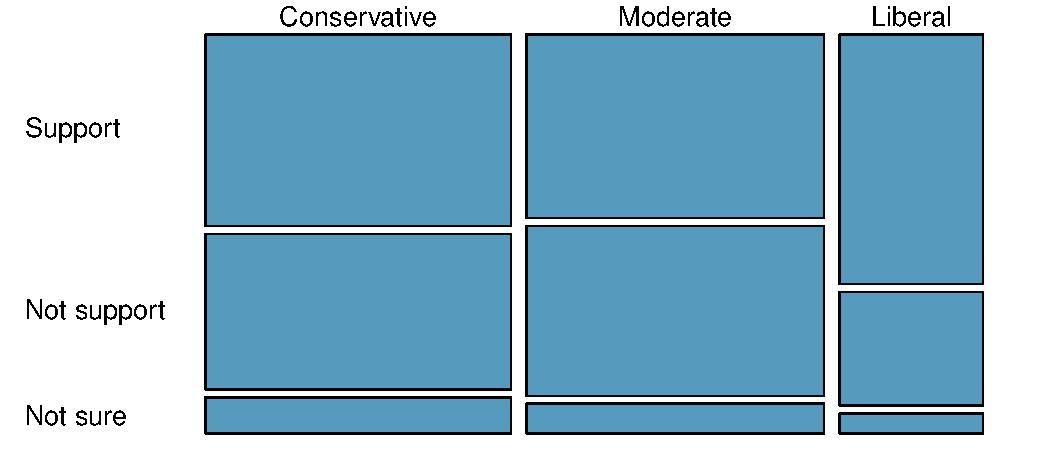
\includegraphics[width = 0.8\textwidth]{ch_summarizing_data/figures/eoce/dream_act_mosaic/dream_act_mosaic.pdf}
\end{center}
}{}

% 40 - raise_taxes_mosaic

\eoce{\qt{Raise taxes\label{raise_taxes_mosaic}} A random sample of registered 
voters nationally were asked whether they think it's better to raise taxes 
on the rich or raise taxes on the poor. The survey also collected information 
on the political party affiliation of the respondents. Based on the mosaic 
plot shown below, do views on raising taxes and  
political affiliation appear to be independent? Explain your reasoning.
\footfullcite{survey:raiseTaxes:2015}
\begin{center}
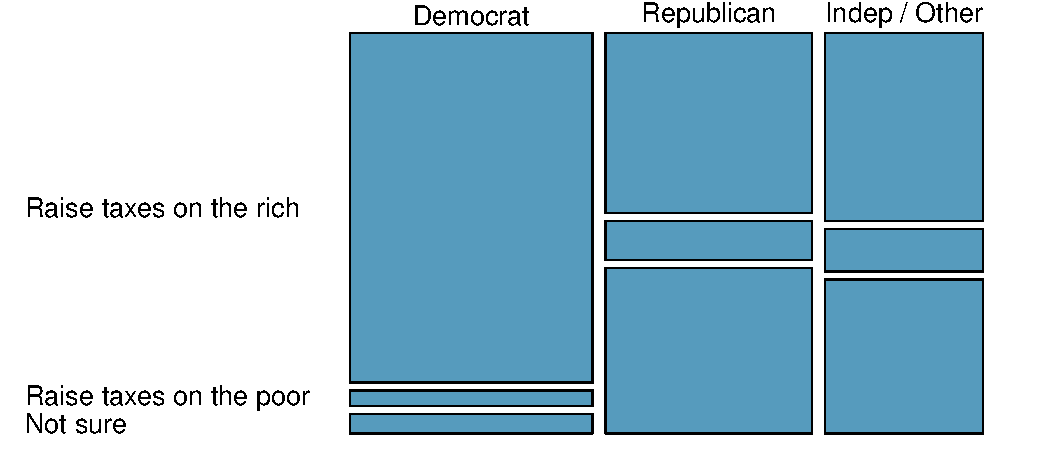
\includegraphics[width = 0.75\textwidth]{ch_summarizing_data/figures/eoce/raise_taxes_mosaic/raise_taxes_mosaic.pdf}
\end{center}
}{}
}



%___________________________________________
\section{Case study: malaria vaccine (special topic)}
\label{caseStudyMalariaVaccine}

\sectionintro{
\noindent%
How large does an observed difference need to be for it to provide convincing evidence that something real is going on, something beyond random variation?  Answering this question requires the tools that we will encounter in the later chapters on probability and inference.
However, this is such an interesting and important question, and we'll also address it here using simulation.
This section can be covered now or in tandem with Chapter~\ref{ch_foundations_for_inf}: Foundations for Inference.


\subsection*{Learning objectives}
\begin{enumerate}
\setlength{\itemsep}{0mm}

\item Recognize that an observed difference in sample statistics may be due to random chance and that we use hypothesis testing to determine if this difference statistically significant (i.e. too large to be attributed to random chance).

\item Set up competing hypotheses and use the results of a simulation to evaluate the degree of support the data provide against the null hypothesis and for the alternative hypothesis.

\end{enumerate}
}


\subsection{Variability within data}
\label{variabilityWithinData}

\index{data!malaria vaccine|(}


\begin{examplewrap}
\begin{nexample}{Suppose your professor splits the students in class into two groups: students on the left and students on the right. If $\hat{p}_{_L}$ and $\hat{p}_{_R}$ represent the proportion of students who own an Apple product on the left and right, respectively, would you be surprised if $\hat{p}_{_L}$ did not {exactly} equal $\hat{p}_{_R}$?}\label{classRightLeftSideApple}
While the proportions would probably be close to each other, it would be unusual for them to be exactly the same. We would probably observe a small difference due to {chance}.
\end{nexample}
\end{examplewrap}

\begin{exercisewrap}
\begin{nexercise}
If we don't think the side of the room a person sits on
in class is related to whether the person owns an Apple product,
what assumption are we making about the relationship between
these two variables?\footnotemark{}
\end{nexercise}
\end{exercisewrap}
\footnotetext{We would be assuming that these two variables
  are independent.}



We consider a study on a new malaria vaccine
called PfSPZ.
In this study, volunteer patients were randomized
into one of two experiment groups:
14 patients received an experimental vaccine
or 6 patients received a placebo vaccine.
Nineteen weeks later, all 20 patients were exposed
to a drug-sensitive malaria virus strain;
the motivation of using a drug-sensitive strain
of virus here is for ethical considerations,
allowing any infections to be treated effectively.
The results are summarized in
Figure~\ref{malaria_vaccine_20_exp_summary},
where 9 of the 14 treatment patients remained free
of signs of infection while all of the~6 patients
in the control group patients showed some baseline
signs of infection.

\D{\newpage}

\newcommand{\malariaAA}{5}
\newcommand{\malariaAB}{9}
\newcommand{\malariaAD}{14}
\newcommand{\malariaBA}{6}
\newcommand{\malariaBB}{0}
\newcommand{\malariaBD}{6}
\newcommand{\malariaDA}{11}
\newcommand{\malariaDB}{9}
\newcommand{\malariaDD}{20}
\newcommand{\malariaVIR}{0.357}
\newcommand{\malariaVIRPerc}{35.7\%}
\newcommand{\malariaPIR}{1.000}
\newcommand{\malariaPIRPerc}{100\%}
\newcommand{\malariaIRDiff}{0.643}
\newcommand{\malariaIRDiffPerc}{64.3\%}

\begin{figure}[ht]
\centering
\begin{tabular}{l l cc rr}
  & & \multicolumn{2}{c}{\var{outcome}} \\
  \cline{3-4}
  &  &  {infection} & {no infection} & Total & \hspace{3mm}  \\ 
  \cline{2-5}
  & {vaccine} &
      \malariaAA{} &
      \malariaAB{} &
      \malariaAD{} \\ 
  \raisebox{1.5ex}[0pt]{\var{treatment}}
  & {placebo} & 
      \malariaBA{} &
      \malariaBB{} &
      \malariaBD{} \\ 
  \cline{2-5}
  & Total & 
      \malariaDA{} &
      \malariaDB{} &
      \malariaDD{} \\ 
  \cline{2-5}
\end{tabular}
\caption{Summary results for the malaria vaccine experiment.}
\label{malaria_vaccine_20_exp_summary}
\end{figure}

\begin{exercisewrap}
\begin{nexercise}
Is this an observational study or an experiment?
What implications does the study type have on what can
be inferred from the results?\footnotemark{}
\end{nexercise}
\end{exercisewrap}
\footnotetext{The
  study is an experiment, as patients were randomly
  assigned an experiment group.
  Since this is an experiment, the results can be used
  to evaluate a causal relationship between the malaria
  vaccine and whether patients showed signs
  of an infection.}

In this study, a smaller proportion of patients
who received the vaccine showed signs of an infection
(\malariaVIRPerc{} versus \malariaPIRPerc{}).
However, the sample is very small,
and it is unclear whether the difference provides
\emph{convincing evidence} that the vaccine is
effective.

\begin{examplewrap}
\begin{nexample}{Data scientists are sometimes called
    upon to evaluate the strength of evidence.
    When looking at the rates of infection for patients
    in the two groups in this study,
    what comes to mind as we try to determine whether
    the data show convincing evidence of a real difference?}
  \label{malaria_vaccine_20_what_is_convincing}
  The observed infection rates
  (\malariaVIRPerc{} for the treatment group versus
  \malariaPIRPerc{} for the control group)
  suggest the vaccine may be effective.
  However, we cannot be sure if the observed difference
  represents the vaccine's efficacy or is just from
  random chance.
  Generally there is a little bit of fluctuation
  in sample data, and we wouldn't expect the sample
  proportions to be \emph{exactly} equal,
  even if the truth was that the infection rates
  were independent of getting the vaccine.
  Additionally, with such small samples,
  perhaps it's common to observe such large differences
  when we randomly split a group due to chance alone!
\end{nexample}
\end{examplewrap}

Example~\ref{malaria_vaccine_20_what_is_convincing}
is a reminder that the observed outcomes in the data
sample may not perfectly reflect the true relationships
between variables since there is \term{random noise}.
While the observed difference in rates of infection
is large, the sample size for the study is small,
making it unclear if this observed difference represents
efficacy of the vaccine or whether it is simply due to
chance.
We label these two competing claims, $H_0$ and $H_A$,
which are spoken as ``H-nought'' and ``H-A'':
\begin{itemize}
\setlength{\itemsep}{0mm}
\item[$H_0$:] \textbf{Independence model.}
    The variables \var{treatment} and \var{outcome}
    are independent.
    They have no relationship, and the observed difference
    between the proportion of patients who developed
    an infection in the two groups, \malariaIRDiffPerc{},
    was due to chance.
\item[$H_A$:] \textbf{Alternative model.}
    The variables are \emph{not} independent.
    The difference in infection rates of
    \malariaIRDiffPerc{}
    was not due to chance,
    and vaccine affected the rate of infection.
\end{itemize}

What would it mean if the independence model,
which says the vaccine had no influence on the
rate of infection, is true?
It would mean 11~patients were going to
develop an infection \emph{no matter which group
they were randomized into},
and 9~patients would not develop an infection
\emph{no matter which group they were randomized
into}.
That~is, if the vaccine did not affect the rate
of infection, the difference in the infection rates
was due to chance alone in how the patients were
randomized.

Now consider the alternative model:
infection rates were influenced by whether a patient
received the vaccine or not.
If this was true, and especially if this influence
was substantial, we would expect to see some difference
in the infection rates of patients in the groups.

We choose between these two competing claims
by assessing if the data conflict so much with
$H_0$ that the independence model cannot be deemed
reasonable.
If this is the case, and the data support $H_A$,
then we will reject the notion of independence
and conclude there was discrimination.


\D{\newpage}

%
\subsection{Simulating the study}
\label{simulatingTheStudy}

We're going to implement
\termsub{simulations}{simulation},
where we will pretend we know that the malaria
vaccine being tested does \emph{not} work.
Ultimately, we want to understand if the large
difference we observed is common in these
simulations.
If it is common, then maybe the difference
we observed was purely due to chance.
If it is very uncommon, then the possibility
that the vaccine was helpful seems more plausible.

Figure~\ref{malaria_vaccine_20_exp_summary}
shows that 11 patients developed infections and 9 did not.
For our simulation, we will suppose the infections
were independent of the vaccine and we were able to
\emph{rewind} back to when the researchers randomized
the patients in the study.
If we happened to randomize the patients differently,
we may get a different result in this hypothetical
world where the vaccine doesn't influence the infection.
Let's complete another \term{randomization} using
a simulation.

In this \term{simulation}, we take 20 notecards to
represent the 20 patients, where we write down ``infection''
on 11 cards and ``no infection'' on 9 cards.
In this hypothetical world, we believe each patient
that got an infection was going to get it regardless
of which group they were in, so let's see what happens
if we randomly assign the patients to the treatment
and control groups again.
We thoroughly shuffle the notecards and deal 14 into
a \resp{vaccine} pile and 6 into a \resp{placebo} pile.
Finally, we tabulate the results, which are shown in
Figure~\ref{malaria_vaccine_20_exp_summary_rand_1}.

\begin{figure}[ht]
\centering
\begin{tabular}{l l cc rr}
  & & \multicolumn{2}{c}{\var{outcome}} \\
  \cline{3-4}
  &  &  {infection} & {no infection} & Total & \hspace{3mm}  \\ 
  \cline{2-5}
  treatment & {vaccine} & 7 & 7 & 14 \\ 
  (simulated) & {placebo} & 4 & 2 & 6 \\ 
  \cline{2-5}
  & Total & 11 & 9 & 20 \\
  \cline{2-5}
\end{tabular}
\caption{Simulation results, where any difference
    in infection rates is purely due to chance.}
\label{malaria_vaccine_20_exp_summary_rand_1}
\end{figure}

\begin{exercisewrap}
\begin{nexercise}
\label{malaria_vaccine_20_exp_summary_rand_1_diff}
What is the difference in infection rates between
the two simulated groups in
Figure~\ref{malaria_vaccine_20_exp_summary_rand_1}?
How does this compare to the observed
\malariaIRDiffPerc{} difference
in the actual data?\footnotemark{}
\end{nexercise}
\end{exercisewrap}
\footnotetext{$4 / 6 - 7 / 14 = 0.167$
  or about 16.7\% in favor of the vaccine.
  This difference due to chance is much smaller than the
  difference observed in the actual groups.}


\subsection{Checking for independence}

We computed one possible difference under the
independence model in Guided
Practice~\ref{malaria_vaccine_20_exp_summary_rand_1_diff},
which represents one difference due to chance.
While in this first simulation, we physically dealt
out notecards to represent the patients,
it is more efficient to perform this simulation
using a computer.
Repeating the simulation on a computer, we get another
difference due to chance:
\begin{align*}
\frac{2}{\malariaBD{}} - \frac{9}{\malariaAD{}} = -0.310
\end{align*}
And another:
\begin{align*}
\frac{3}{\malariaBD{}} - \frac{8}{\malariaAD{}} = -0.071
\end{align*}
And so on until we repeat the simulation enough times
that we have a good idea of what represents the
\emph{distribution of differences from chance alone}.
Figure~\ref{malaria_rand_dot_plot} shows a stacked plot
of the differences found from 100 simulations,
where each dot represents a simulated difference between
the infection rates (control rate minus treatment rate).

\begin{figure}[ht]
  \centering
  \Figure{0.74}{malaria_rand_dot_plot}
  \caption{A stacked dot plot of differences from
      100 simulations produced under the independence model,
      $H_0$, where in these simulations infections are
      unaffected by the vaccine.
      Two of the 100 simulations had a difference of
      at least \malariaIRDiffPerc{}, the difference observed
      in the study.}
  \label{malaria_rand_dot_plot}
\end{figure}

Note that the distribution of these simulated differences
is centered around 0.
We simulated these differences assuming that the independence
model was true, and under this condition,
we expect the difference to be near zero with some random
fluctuation, where \emph{near} is pretty generous in this
case since the sample sizes are so small in this study.

\begin{examplewrap}
\begin{nexample}{Given the results of the simulation shown in Figure~\ref{malaria_rand_dot_plot}, about how often would you expect to observe a result as large as \malariaIRDiffPerc{} if $H_0$ were true?} 
  Because a result this large happened 2 times out the 100 simulations, we would expect such a large value only 2\% of the time if $H_0$ were true.  
\end{nexample}
\end{examplewrap}

There are two possible interpretations
of the results of the study:
\begin{itemize}
  \setlength{\itemsep}{0mm}
  \item[$H_0$] \textbf{Independence model.}
      The vaccine has no effect on infection rate,
      and we just happened to observe a rare event.
  \item[$H_A$] \textbf{Alternative model.}
      The vaccine has an effect on infection rate,
      and the difference we observed was actually due to
      the vaccine being effective at combatting malaria,
      which explains the large difference
      of~\malariaIRDiffPerc{}.
\end{itemize}
Based on the simulations, we have two options.
(1)~We conclude that the study results do not provide
strong enough evidence against the independence model,
meaning we do not conclude that the vaccine had an effect
in this clinical setting.
(2)~We conclude the evidence is sufficiently strong
to reject $H_0$, and we assert that the vaccine was useful.

Is 2\% small enough to make us reject the independence model?  That depends on how much evidence we require.  The smaller that probability is, the more evidence it provides against $H_0$.  Later, we will see that researchers often use a cutoff of 5\%, though it can depend upon the situation.
Using the 5\% cutoff, we would reject the independence model in favor
of the alternative.
That is, we are concluding the data provide strong evidence
that the vaccine provides some protection against malaria
in this clinical setting. 

When there is strong enough evidence that the result points to a real difference and is not simply due to random variation, we call the result \term{statistically significant}.

\index{data!malaria vaccine|)}

One field of statistics, statistical inference, is built
on evaluating whether such differences are due to chance.
In statistical inference, data scientists evaluate which
model is most reasonable given the data.
Errors do occur, just like rare events, and we might choose
the wrong model.
While we do not always choose correctly, statistical
inference gives us tools to control and evaluate how
often these errors occur.
In Chapter~\ref{foundationsForInference},
we give a formal introduction to the problem of model
selection.
We spend the next two chapters building a foundation
of probability and theory necessary to make that
discussion rigorous.



%%%%%%Section Exercises
{\exercisesheader{}

% 41 - randomization_avandia

\eoce{\qt{Side effects of Avandia\label{randomization_avandia}} Rosiglitazone is the 
active ingredient in the controversial type~2 diabetes medicine Avandia and has 
been linked to an increased risk of serious cardiovascular problems such as 
stroke, heart failure, and death. A common alternative treatment is pioglitazone, 
the active ingredient in a diabetes medicine called Actos. In a nationwide 
retrospective observational study of 227,571 Medicare beneficiaries aged  
65 years or older, it was found that 2,593 of the 67,593 patients using 
rosiglitazone and 5,386 of the 159,978 using pioglitazone had serious 
cardiovascular problems. These data are summarized in the contingency 
table below. \footfullcite{Graham:2010}
\begin{center}
\begin{tabular}{ll  cc c} 
                                &   & \multicolumn{2}{c}{\textit{Cardiovascular problems}} \\
\cline{3-4} 
                                    &               & Yes   & No        & Total \\
\cline{2-5}
\multirow{2}{*}{\textit{Treatment}} & Rosiglitazone & 2,593 & 65,000    & 67,593 \\
                                    & Pioglitazone  & 5,386 & 154,592   & 159,978 \\
\cline{2-5}
                                    & Total         & 7,979 & 219,592   & 227,571
\end{tabular}
\end{center}
\begin{parts}
\item Determine if each of the following statements is true or false. If false, explain why. \textit{Be careful:} The reasoning may be wrong even if the statement's conclusion is correct. In such cases, the statement should be considered false.
\begin{subparts}
\item Since more patients on pioglitazone had cardiovascular problems (5,386 vs. 2,593), we can conclude that the rate of cardiovascular problems for those on a pioglitazone treatment is higher.
\item The data suggest that diabetic patients who are taking rosiglitazone are more likely to have cardiovascular problems since the rate of incidence was (2,593 / 67,593 = 0.038) 3.8\% for patients on this treatment, while it was only (5,386 / 159,978 = 0.034) 3.4\% for patients on pioglitazone.
\item The fact that the rate of incidence is higher for the rosiglitazone group proves that rosiglitazone causes serious cardiovascular problems.
\item Based on the information provided so far, we cannot tell if the difference between the rates of incidences is due to a relationship between the two variables or due to chance.
\end{subparts}
\item What proportion of all patients had cardiovascular problems?
\item If the type of treatment and having cardiovascular problems were independent, about how many patients in the rosiglitazone group would we expect to have had cardiovascular problems?
\item We can investigate the relationship between outcome and treatment in this study using a randomization technique.  While in reality we would carry out the simulations required for randomization using statistical software, suppose we actually simulate using index cards. In order to simulate from the independence model, which states that the outcomes were independent of the treatment, we write whether or not each patient had a cardiovascular problem on cards, shuffled all the cards together, then deal them into two groups of size 67,593 and 159,978. We repeat this simulation 1,000 times and each time record the number of people in the rosiglitazone group who had cardiovascular problems. Use the relative frequency histogram of these counts to answer (i)-(iii).
\end{parts}
\begin{minipage}[c]{0.5\textwidth}
\begin{subparts}
\item What are the claims being tested?
\item Compared to the number calculated in part (b), which would provide more support for the alternative hypothesis,  \textit{more} or \textit{fewer} patients with cardiovascular problems in the rosiglitazone group?
\item What do the simulation results suggest about the relationship between taking rosiglitazone and having cardiovascular problems in diabetic patients?
\end{subparts}
\end{minipage}
\begin{minipage}[c]{0.5\textwidth}
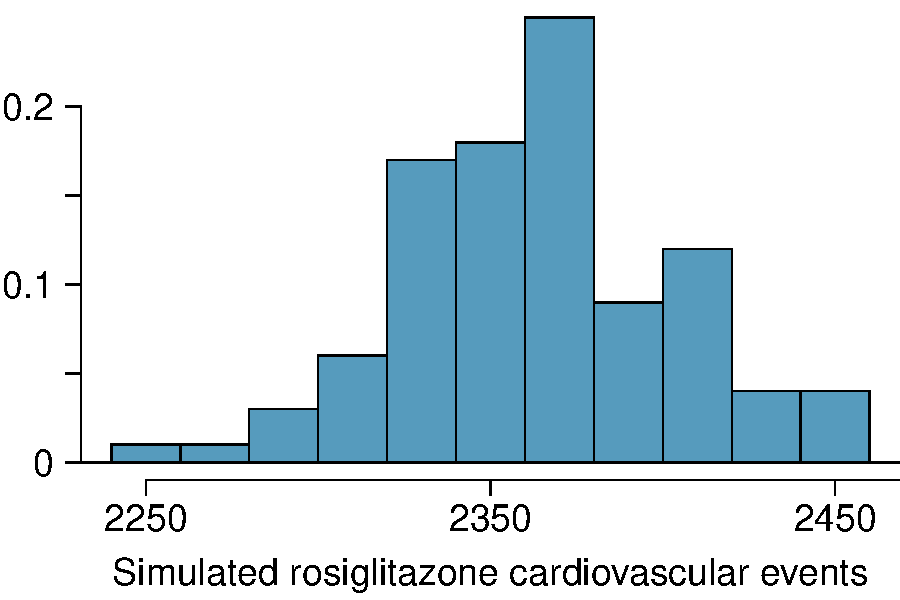
\includegraphics[width = \textwidth]{ch_summarizing_data/figures/eoce/randomization_avandia/randomization_avandia.pdf} \\
\end{minipage}
}{}

% 42 - randomization_heart_transplants

\eoce{\qt{Heart transplants\label{randomization_heart_transplants}} The Stanford 
University Heart Transplant Study was conducted to determine whether an 
experimental heart transplant program increased lifespan. Each patient 
entering the program was designated an official heart transplant candidate, 
meaning that he was gravely ill and would most likely benefit from a new heart. 
Some patients got a transplant and some did not. The variable \texttt{transplant} 
indicates which group the patients were in; patients in the treatment group got a 
transplant and those in the control group did not. Of the 34 patients in the 
control group, 30 died. Of the 69 people in the treatment group, 45 died. Another 
variable called \texttt{survived} was used to indicate whether or not the patient 
was alive at the end of the study. \footfullcite{Turnbull+Brown+Hu:1974}
\begin{center}
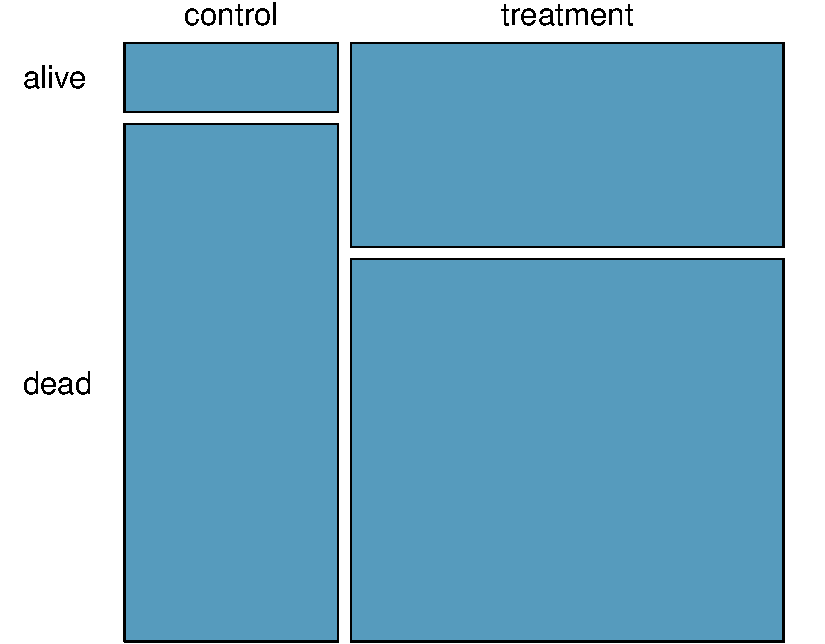
\includegraphics[width= 0.48\textwidth]{ch_summarizing_data/figures/eoce/randomization_heart_transplants/randomization_heart_transplants_mosaic.pdf}
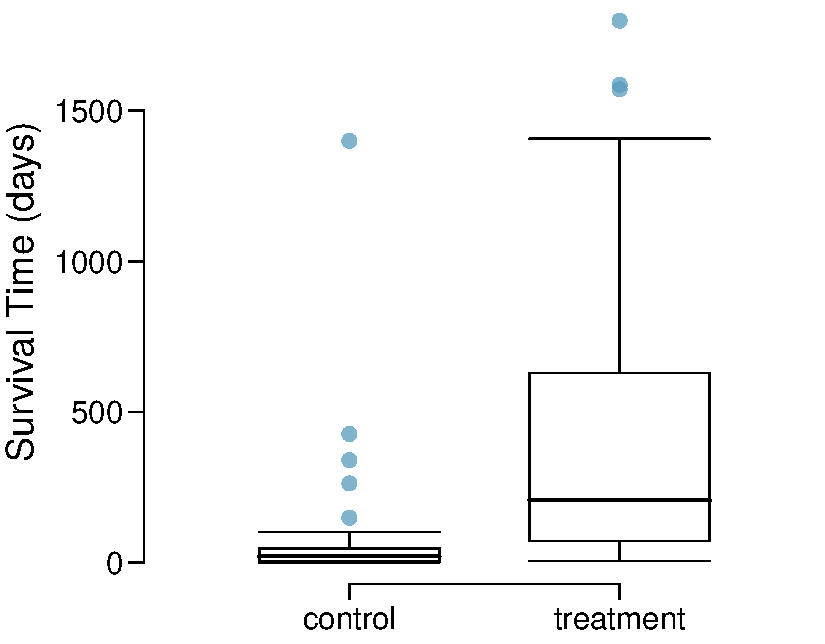
\includegraphics[width= 0.48\textwidth]{ch_summarizing_data/figures/eoce/randomization_heart_transplants/randomization_heart_transplants_box.pdf}
\end{center}
\begin{parts}
\item Based on the mosaic plot, is survival independent of whether or not the 
patient got a transplant? Explain your reasoning.
\item What do the box plots below suggest about the efficacy (effectiveness) of the heart transplant treatment.
\item What proportion of patients in the treatment group and what proportion of 
patients in the control group died?
\item One approach for investigating whether or not the treatment is effective 
is to use a randomization technique.
\begin{subparts}
\item What are the claims being tested?
\item The paragraph below describes the set up for such approach, if we were 
to do it without using statistical software. Fill in the blanks with a number 
or phrase, whichever is appropriate.
\begin{adjustwidth}{2em}{2em}
We write \textit{alive} on \rule{2cm}{0.5pt} cards representing patients who were 
alive at the end of the study, and \textit{dead} on \rule{2cm}{0.5pt} cards 
representing patients who were not. Then, we shuffle these cards and split them 
into two groups: one group of size \rule{2cm}{0.5pt} representing treatment, and 
another group of size \rule{2cm}{0.5pt} representing control. We calculate the 
difference between the proportion of \textit{dead} cards in the treatment and 
control groups (treatment - control) and record this value. We repeat this 100 
times to build a distribution centered at \rule{2cm}{0.5pt}. Lastly, we calculate 
the fraction of simulations where the simulated differences in proportions are 
\rule{2cm}{0.5pt}. If this fraction is low, we conclude that it is unlikely to 
have observed such an outcome by chance and that the null hypothesis should 
be rejected in favor of the alternative.
\end{adjustwidth}
\item What do the simulation results shown below suggest about the effectiveness 
of the transplant program?
\end{subparts}
\end{parts}
\begin{center}
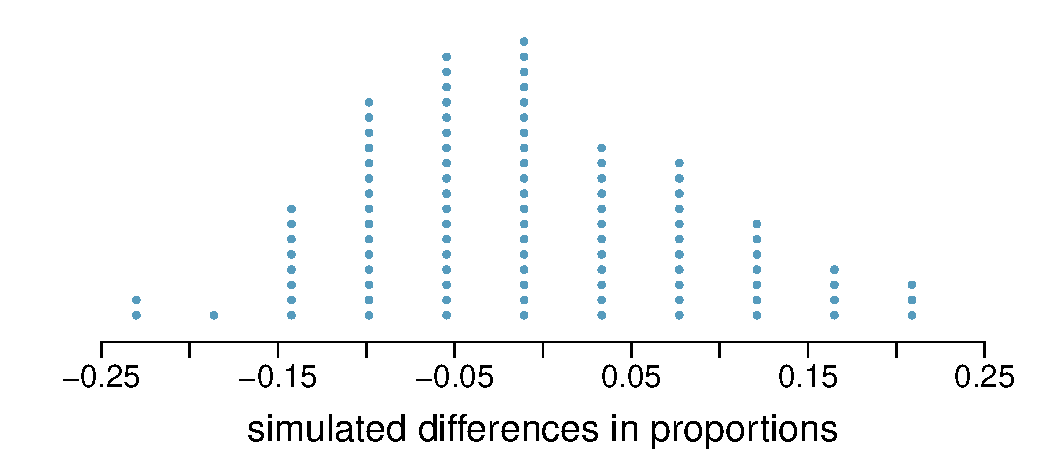
\includegraphics[width= 0.6\textwidth]{ch_summarizing_data/figures/eoce/randomization_heart_transplants/randomization_heart_transplants_rando.pdf}
\end{center}
}{}
}


%______________________________________________
\reviewchapterheader{}

\noindent A raw data matrix/table may have thousands of rows.  The data need to be summarized in order to makes sense of all the information.  In this chapter, we looked at ways to summarize data \term{graphically}, \term{numerically}, and \term{verbally}.  
\\
\\\termsub{Categorical data}{categorical}
\begin{itemize}
\item A single \term{categorical variable} is summarized with \term{counts} or \termsub{proportions}{proportion} in a \term{one-way table}.  A \term{bar~chart} is used to show the frequency or relative frequency of the categories that the variable takes on.
\item Two categorical variables can be summarized in a \term{two-way table} and with a \term{side-by-side bar~chart} or a \term{segmented bar~chart}.
\end{itemize}
\termsub{Numerical data}{numerical data}
\begin{itemize}
\item When looking at a single \term{numerical variable}, we try to understand the \term{distribution} of the variable.  The distribution of a variable can be represented with a frequency table and with a graph, such as a \term{stem-and-leaf plot} or \term{dot plot} for small data sets, or a \term {histogram} for larger data sets.  If only a summary is desired, a \term{box plot} may be used.
\item The \term{distribution} of a variable can be described and summarized with \term{center} (mean or median), \term{spread} (SD or IQR), and \term{shape} (right skewed, left skewed, approximately symmetric). 
\item \termsub{Z-scores}{Z-score} and \termsub{percentiles}{percentile} are useful for identifying a data point's relative position within a data set.
\item \termsub{Outliers}{outlier} are values that appear extreme relative to the rest of the data.  Investigating outliers can provide insight into properties of the data or may reveal data collection/entry errors.
\item When \termsub{comparing the distribution}{comparing distributions} of two variables, use two dot plots, two histograms, a back-to-back stem-and-leaf, or parallel box plots.
\item To look at the \term{association} between two numerical variables, use a \term{scatterplot}.
\end{itemize}
Graphs and numbers can summarize data, but they alone are insufficient.  It is the role of the researcher or data scientist to ask questions, to use these tools to identify patterns and departure from patterns, and to make sense of this in the context of the data.  Strong writing skills are critical for being able to communicate the results to a wider audience.  

